\documentclass{wissdoc}

% ----------------------------------------------------------------
%    My Information
% ----------------------------------------------------------------

\newcommand{\myname}{Lucas~Czech}
\newcommand{\mytitle}{Novel Methods for Post-Processing Evolutionary Data Using Machine Learning Techniques}
% \newcommand{\myinstitute}{Institute for Program Structures\\and Data Organization (IPD)}

\newcommand{\reviewerone}{Prof.~Dr.~Alexandros~Stamatakis}
\newcommand{\reviewertwo}{Prof.~Dr.~Emmanuel~Müller}
\newcommand{\advisorone}{}
\newcommand{\advisortwo}{}

\newcommand{\timestart}{July 1, 2014}
\newcommand{\timeend}{September 30, 2018}
\newcommand{\submissiontime}{September 30, 2018}
\newcommand{\submissionlocation}{Karlsruhe}

\author{\myname}
\title{\mytitle}

%% Informationen für die PDF-Datei
\pdfstringdefDisableCommands{\def\\#1{ #1}}
\hypersetup{
	pdfauthor={\myname},
	pdftitle={\mytitle},
	pdfsubject={In this work, we present a system for recognizing spelled speech in English that supports phrases like "A as in alpha".},
	pdfkeywords={automatic speech recognition, spelling, English, phrases, NATO alphabet, confusion network, depth first search, beam search, letters, alphabets}
}

% ----------------------------------------------------------------
%    Customization
% ----------------------------------------------------------------

\newcommand\todo[1]{{\color{purple}{TODO: #1}}}

% Define custom styles
\newcommand\toolname{\textsc}
\newcommand\taxonname{\textit}
\newcommand\fileformat{\texttt}

\newcommand\tabref[1]{Table~\ref{#1}}
\newcommand\figref[1]{Figure~\ref{#1}}
% \newcommand\suppfigref[1]{S\ref{#1}~Fig}

% ART Paper
\newcommand\paperart{
    \item \textbf{Lucas Czech}, Pierre Barbera, and Alexandros Stamatakis.
        "Methods for Automatic Reference Trees and Multilevel Phylogenetic Placement."
        \textit{Bioinformatics}, 2018.
}

% Phylogenetic Postprocessing Paper
\newcommand\paperpppp{
    \item \textbf{Lucas Czech} and Alexandros Stamatakis.
        "Scalable Methods for Post-Processing, Visualizing, and Analyzing Phylogenetic Placements."
        \textit{PLOS One}, 2018.
}

% Command for framed boxes.
\newcommand\paperbox[3]{
    \begin{framed}
    % \noindent
    #1
    \begin{itemize}
        #2
    \end{itemize}
    % \noindent
    #3
    \end{framed}
}

% https://tex.stackexchange.com/a/5255
\DeclareMathOperator*{\argmax}{arg\,max}

% ----------------------------------------------------------------
%    Settings
% ----------------------------------------------------------------

% ------------------------------------------
%  Text editing
% ------------------------------------------

\newcommand\todo[1]{{\color{purple}{TODO: #1}}}

% ------------------------------------------
%  Custom styles
% ------------------------------------------

\newcommand\toolname{\textsc}
\newcommand\taxonname{\textit}
\newcommand\fileformat{\texttt}
\newcommand\nucleobase[1]{\texttt{#1}}

% Epigraph
% https://tex.stackexchange.com/questions/193178/specific-epigraph-style
\usepackage{epigraph}
\setlength\epigraphwidth{.8\textwidth}
\setlength\epigraphrule{0pt}

% ------------------------------------------
%  References
% ------------------------------------------

\newcommand\secref[1]{Section~\ref{#1}}
\newcommand\figref[1]{Figure~\ref{#1}}
% \newcommand\suppfigref[1]{S\ref{#1}~Fig}
\newcommand\tabref[1]{Table~\ref{#1}}
\renewcommand\algref[1]{Algorithm~\ref{#1}}
\newcommand\eqnref[1]{Equation~\ref{#1}}

% ------------------------------------------
%  abbreviations
% ------------------------------------------

\def\eg{e.\,g.\ }
\def\ie{i.\,e.\ }
\def\cf{c.\,f.\ }

\DeclareSIUnit\basepair{bp}

% Remove hyperlink color boxes from acronyms.
% https://tex.stackexchange.com/questions/73063/acronym-hyperlink-without-special-color/73068
\makeatletter
\AtBeginDocument{%
  \renewcommand*{\AC@hyperlink}[2]{%
    \begingroup
      \hypersetup{hidelinks}%
      \hyperlink{#1}{#2}%
    \endgroup
  }%
}
\makeatother

% ------------------------------------------
%  Math operators
% ------------------------------------------

\def\avg{\mathop{\mathgroup\symoperators avg}}

% https://tex.stackexchange.com/a/5255
\DeclareMathOperator*{\argmax}{arg\,max}

% ------------------------------------------
%  Page Handling
% ------------------------------------------

% Leerseite, nächste Seite rechts
\newcommand{\blankpage}{
 \clearpage{\pagestyle{fancy}\cleardoublepage}
}

% marker for lowercase references
% (see http://tex.stackexchange.com/questions/1655/correct-case-in-namerefs)
\newcommand{\mlr}{}

% use marker to define lowercase reference command...
\newcommand{\lnameref}[1]{%
\bgroup
\let\mlr\MakeLowercase
\nameref{#1}\egroup}

% ... and first upper, rest lowercase command
\newcommand{\fnameref}[1]{%
\bgroup
\def\mlr{\let\mlr\MakeLowercase}%
\nameref{#1}\egroup}

% ------------------------------------------
%  Papers References and Boxes
% ------------------------------------------

% ART Paper
\newcommand\paperart{
    \item \textbf{Lucas Czech}, Pierre Barbera, and Alexandros Stamatakis.
        "Methods for Automatic Reference Trees and Multilevel Phylogenetic Placement."
        \textit{Bioinformatics}, 2018.
}

% Phylogenetic Postprocessing Paper
\newcommand\paperpppp{
    \item \textbf{Lucas Czech} and Alexandros Stamatakis.
        "Scalable Methods for Post-Processing, Visualizing, and Analyzing Phylogenetic Placements."
        \textit{PLOS One}, 2018.
}

% Command for framed boxes.
\newcommand\paperbox[3]{
    \begin{framed}
    % \noindent
    #1
    \begin{itemize}
        #2
    \end{itemize}
    % \noindent
    #3
    \end{framed}
}

\graphicspath{{pdf/}}

% Trennhilfen
% Wichtig!
% Im ngerman-paket sind zusätzlich folgende Trennhinweise enthalten:
% "- = zusätzliche Trennstelle
% "| = Vermeidung von Ligaturen und mögliche Trennung (bsp: Schaf"|fell)
% "~ = Bindestrich an dem keine Trennung erlaubt ist (bsp: bergauf und "~ab)
% "= = Bindestrich bei dem Worte vor und dahinter getrennt werden dürfen
% "" = Trennstelle ohne Erzeugung eines Trennstrichs (bsp: und/""oder)
\hyphenation{
}

% Index-Datei öffnen
\makeindex

% ----------------------------------------------------------------
%    Main Document
% ----------------------------------------------------------------

\begin{document}

\frontmatter
\pagenumbering{roman}

\begin{titlepage}
\thispagestyle{empty}
\setlength{\unitlength}{1pt}

%% ==============================
% Spacing
%% ==============================

% title page space big/small
\newcommand{\tpsb}{\vskip 2.8cm}
\newcommand{\tpss}{\vskip 1.0cm}
\newcommand{\tpsm}{\vskip 0.5cm}

%% ==============================
% Title
%% ==============================

% \begin{picture}(0,0)(85,770)
% % \includegraphics[width=\paperwidth]{logos/KIT_Deckblatt_neu.pdf}
% \includegraphics[width=\paperwidth]{logos/titlepage.pdf}
% \end{picture}

\begin{center}
\hbox{}
% \vfill

% \tpsb
% \tpss
{\huge\bfseries \mytitle \par}
\tpss
% Dissertation\\by\\%[2mm]
zur Erlangung des akademischen Grades eines
\tpss
{\Large
Doktors der Ingenieurwissenschaften /
\\
Doktors der Naturwissenschaften
}
\tpss
der KIT-Fakultät für Informatik \\
des Karlsruher Instituts für Technologie (KIT)
\tpss
\textbf{vorgelegte} \\
% \tpsm
% (vor der mündlichen Promotionsprüfung)
\begin{large}\textbf{Dissertation}\end{large}
\tpsm
von
\tpsm
% {\large\bfseries \myname}
\begin{large}\textbf{\myname}\end{large} \\
% \tpsm
aus \mycity
\tpss

%% ==============================
% Institute
%% ==============================

% \tpss
% at the\\
% Interactive Systems Labs (ISL)%\\ \vspace*{1em}
% Institute for Anthropomatics,\\
%der Fakultät für Informatik\\
% At the Department of Informatics
% An der Fakult\"at f\"ur Informatik
% Department of Informatics,
% Karlsruhe Institute of Technology (KIT),\\
% Karlsruhe, Germany

% Heidelberg Institute for Theoretical Studies (HITS),\\
% Heidelberg, Germany
% 
%International Center for Advanced  Communication Technologies

% \begin{tabular}{p{8.5cm}l}
%   Interactive Systems Labs (ISL)		& interACT, \\
%   Institute for Anthropomatics,,		& Language Technologies Institute (LTI), \\
%   Department of Informatics,			& School of Computer Science, \\
%   Karlsruhe Institute of Technology (KIT), 	& Carnegie Mellon University (CMU) \\
%   Karlsruhe, Germany 				& Pittsburgh, USA \\
% \end{tabular}

% \begin{tabular}{p{12cm}}
% 	at the \\
% 	Interactive Systems Labs (ISL) \\
% 	Karlsruhe Institute of Technology (KIT), Karlsruhe, Germany \\
% 	Carnegie Mellon University (CMU) Pittsburgh, USA
% \end{tabular}

%% ==============================
% Reviewers
%% ==============================

  % Gutachter sind die Professoren, die die Arbeit bewerten.
  % Der zweite betreuende Mitarbeiter kann weggelassen werden.

\tpsb
\begin{center}
\begin{tabular}{p{7.0cm}p{7.0cm}}
%   First Reviewer: & \reviewerone \\
%   Second Reviewer: & \reviewertwo \\
%   Advisor: & \advisorone \\
%   Second Advisor: & \advisortwo \\
Tag der mündlichen Prüfung: & \submissiontime \\
Erster Gutachter: & \reviewerone \\
Zweiter Gutachter: & \reviewertwo \\
\end{tabular}
\end{center}

%% ==============================
% Footer
%% ==============================

% \tpss
% \qquad \timestart ~-- \timeend
% \timeend

\end{center}
\vfill
\end{titlepage}

\blankpage

\selectlanguage{ngerman}
%\begin{abstract}
\section*{Zusammenfassung}
\vspace*{1em}

Auf deutsch...

%\end{abstract}
\blankpage

\selectlanguage{english}
%\begin{abstract}
\section*{Abstract}
\vspace*{1em}

In English...

%\end{abstract}

\blankpage

% \thispagestyle{empty}
% \vspace*{42\baselineskip}
% \hbox to \textwidth{\hrulefill}
% \par
% Ich erkläre hiermit, dass ich die vorliegende Arbeit selbständig verfasst und
% keine anderen als die angegebenen Quellen und Hilfsmittel verwendet habe.
%
% Karlsruhe, den ??. ?????? 201?
%
% %%%%%%%%%%%%%%%%%%%%%%%%%%%%%%%%%%%%%%%%%%%%%%%%%%%%%%%%%%%%%%%%%%%%%%%%
% %% Hinweis:
% %%
% %% Diese Erklärung wird von der Prüfungsordnung für Diplomarbeiten
% %% verlangt und ist zu unterschreiben. Für Studienarbeiten ist diese
% %% Erklärung nicht zwingend notwendig, schadet aber auch nicht.
% %%%%%%%%%%%%%%%%%%%%%%%%%%%%%%%%%%%%%%%%%%%%%%%%%%%%%%%%%%%%%%%%%%%%%%%%
% \clearpage

\thispagestyle{empty}
\vspace*{33\baselineskip}
\hbox to \textwidth{\hrulefill}
\par

%I hereby declare that I have developed and written the enclosed thesis completely by myself, and have not used sources or means without declaration in the text.

%Ich versichere wahrheitsgem\"a\ss, die Arbeit selbstst\"andig angefertigt, alle benutzten Hilfsmittel vollst\"andig und genau angegeben und alles kenntlich gemacht zu haben, was aus Arbeiten anderer unver\"andert oder mit Ab\"anderungen entnommen wurde.

Hiermit erkläre ich, dass ich diese Arbeit selbständig angefertigt und keine anderen als
die angegebenen Quellen und Hilfsmittel benutzt sowie die wörtlich oder inhaltlich
übernommenen Stellen als solche kenntlich gemacht habe. Ich habe die Satzung
des Karlsruher Institutes für Technologie (KIT) zur Sicherung guter wissenschaftlicher Praxis beachtet.

\textbf{\submissionlocation, \submissiontime}
\vspace{1.5cm}

\dotfill\hspace*{8.0cm}\\
\hspace*{2cm}(\textbf{\myname}) %center name with hspace

\blankpage

\section*{Acknowledgment}
\vspace*{1em}

\epigraph
{\textit{``Evolution forged the entirety of [...] life on this planet \\ using only one tool -- the mistake.''}}
{--- Dr. Robert Ford (Anthony Hopkins),\\ \textit{Westworld, Season 1: The Original}}


falsification, science ``irrt sich vorwaerts''... mein beitrag, aber nicht ohne die hilfe vieler anderer


There are many people who helped and supported me in different ways during the conduction of this dissertation.

First, I would like to thank my advisor Professor Dr. Alexandros Panavotis Stamatakis,

Many thanks also to my second advisor Professor Dr. Emmanuel Müller for his support and advice.

also, other reviewers and examiners of my thesis and work.

To the team of the Exelixis Lab--- namely ... --- also many thanks, you made ....
andre, paschalia, tomas, diego, jiajie, kassian

mark, emily, jaime, fred, micah, cedric, colomban, pelin

Finally, I want to thank my parents Peter and Maria and my sister Judith,
who not only constantly supported me during this thesis,
but through all of my years of study in Karlsruhe, Heidelberg and around the world.


This work was financially supported by the \textbf{Klaus Tschira Stiftung gGmbH} in Heidelberg, Germany.
HITS, KIT

We thank \textbf{S. Srinivasan} and \textbf{E. Matsen}
for providing the Bacterial Vaginosis dataset \cite{Srinivasan2012}
and for helping us understanding their methods and implementations.
We also thank \textbf{M. Dunthorn}, \textbf{L. Rubinat-Ripoll}, \textbf{C. Berney}, \textbf{L. Guidi},
\textbf{G. Lentendu}, %\textbf{S. Filker},
\textbf{A. Kozlov}, and \textbf{P. Barbera}
for their feedback on our methods and help with this manuscript.

We thank \textbf{S.~Srinivasan} and \textbf{E.~Matsen}
for providing the Bacterial Vaginosis dataset \citep{Srinivasan2012};
\textbf{M.~Dunthorn}, \textbf{G.~Lentendu}, %\textbf{P.~Barbera}
and \textbf{A.~Kozlov}
for their feedback on our methods and this manuscript.

thanks also to the (mostly) anonymous reviewers of our publications,
who pointed out flaws to us and thus helped to make them better.


phil collins peter gabriel

richard dawkins, ohne den ich nicht auf das thema aufmerksam geworden waere und daher nicht mit der phd stelle angefangen haette.

not to forget:
\url{https://xkcd.com/1706/}

or maybe:
\url{https://www.xkcd.com/1840/}

or better:
\url{https://xkcd.com/1605/}

% Thanks to all of you!

% Widmungen
% • Danksagungen
% • Persönlicher Bezug zum Thema
% • Nennung und Würdigung der externen Institutionen
% • und den entsprechenden Ansprechpartnern vor Ort

% \begin{center}
% 	\includegraphics[width=1.0\textwidth,keepaspectratio=true]{./logos/bild_logo_bwsbwstiftung.jpg}
% \end{center}
% \vspace{-6cm}

% \vspace*{3em}
% \vfil
% \hspace{2.2cm}\includegraphics[width=0.4\textwidth,keepaspectratio=true]{./logos/interACT_pix.jpg}
% \hspace{2.3cm}\includegraphics[width=0.4\textwidth,keepaspectratio=true]{./logos/logo_interact_4c2.pdf}
% \vspace{0cm}
% \begin{center}
% 	\includegraphics[width=1.0\textwidth,keepaspectratio=true]{./logos/B_ed1cad28a0.png}
% \end{center}

\blankpage

% ------------------------------------------
%    Directories
% ------------------------------------------

{\parskip 0pt\tableofcontents}
\blankpage

{\parskip 0pt\listoffigures}
\blankpage

{\parskip 0pt\listoftables}
\blankpage

% {\parskip 0pt\listofalgorithms}
% \blankpage

\chapter*{List of Acronyms}
\begin{acronym}
    \acro{RT}[RT]{reference tree}
%     \acroplural{RT}[RTs]{reference trees}
    \acro{RA}[RA]{reference alignment}
%     \acroplural{RA}[RAs]{reference alignment}
    \acro{QS}[QS]{query sequence}
%     \acroplural{QS}[QSs]{query sequences}

    \acro{BT}[BT]{backbone tree}
%     \acroplural{BT}[BTs]{backbone trees}
    \acro{CT}[CT]{clade tree}
%     \acroplural{CT}[CTs]{clade trees}

    \acro{LWR}[LWR]{likelihood weight ratio}
%     \acroplural{LWR}[LWRs]{likelihood weight ratios}

    \acro{ART}[ART]{automatic reference tree}

    \acro{PCA}[PCA]{Principal Components Analysis}
    \acro{MDS}[MDS]{Multidimensional scaling}

    \acro{BV}[BV]{Bacterial Vaginosis}
    \acro{NTS}[NTS]{Neotropical Soils}
    \acro{TO}[TO]{Tara Oceans}
    \acro{HMP}[HMP]{Human Microbiome Project}
\end{acronym}
\blankpage

% ------------------------------------------
%    Main Part
% ------------------------------------------

\mainmatter
\pagenumbering{arabic}

% ######################################################################################################################
%         Introduction
% ######################################################################################################################

\chapter{Introduction}
\label{ch:Introduction}

% ######################################################################################################################
%         Background and Motivation
% ######################################################################################################################

\section{Background and Motivation}
\label{ch:Introduction:sec:Motivation}

The concept of evolution is the cornerstone of modern biology \cite{Dobzhansky1973}.
% \secref{ch:Foundations:sec:EvolutionGenetics}
All life on earth descends from a common ancestor and continuously evolves over generations,
which leads to a diversification of biological species.
The resulting branching pattern of the evolutionary relationships between species
is the key for unraveling many biological questions.
These evolutionary relationships are described by \emph{phylogenetic trees}
(\secref{ch:Foundations:sec:TreeOfLife}),
which are important in both basic \cite{Misof2014,Jarvis2014,Zanne2014} and
applied research \cite{Futuyma1995,Hendry2011,Schwartz2017}.

Characteristics and traits of biological species are inherited via their DNA
(\secref{ch:Foundations:sec:EvolutionGenetics}).
DNA data is hence often used for inferring a phylogenetic tree for a set of species
(\secref{ch:Foundations:sec:MLTreeInference}).
In order to conduct such analyses, the DNA has to be sequenced,
that is, it has to be ``read'' into some human-accessible format,
typically in form of a sequence of characters
(\secref{ch:Foundations:sec:SequenceAnalysis}).
In recent decades, the throughput of sequencing technologies increased,
while at the same time, the cost decreased faster than Moore's law,
as shown in \figref{fig:sequencing_costs}.
This lead to a ``tsunami'' of sequence data,
which constitutes a challenge for computational analyses of these data.
% computational biology

\begin{figure}[hbt]
    \centering
    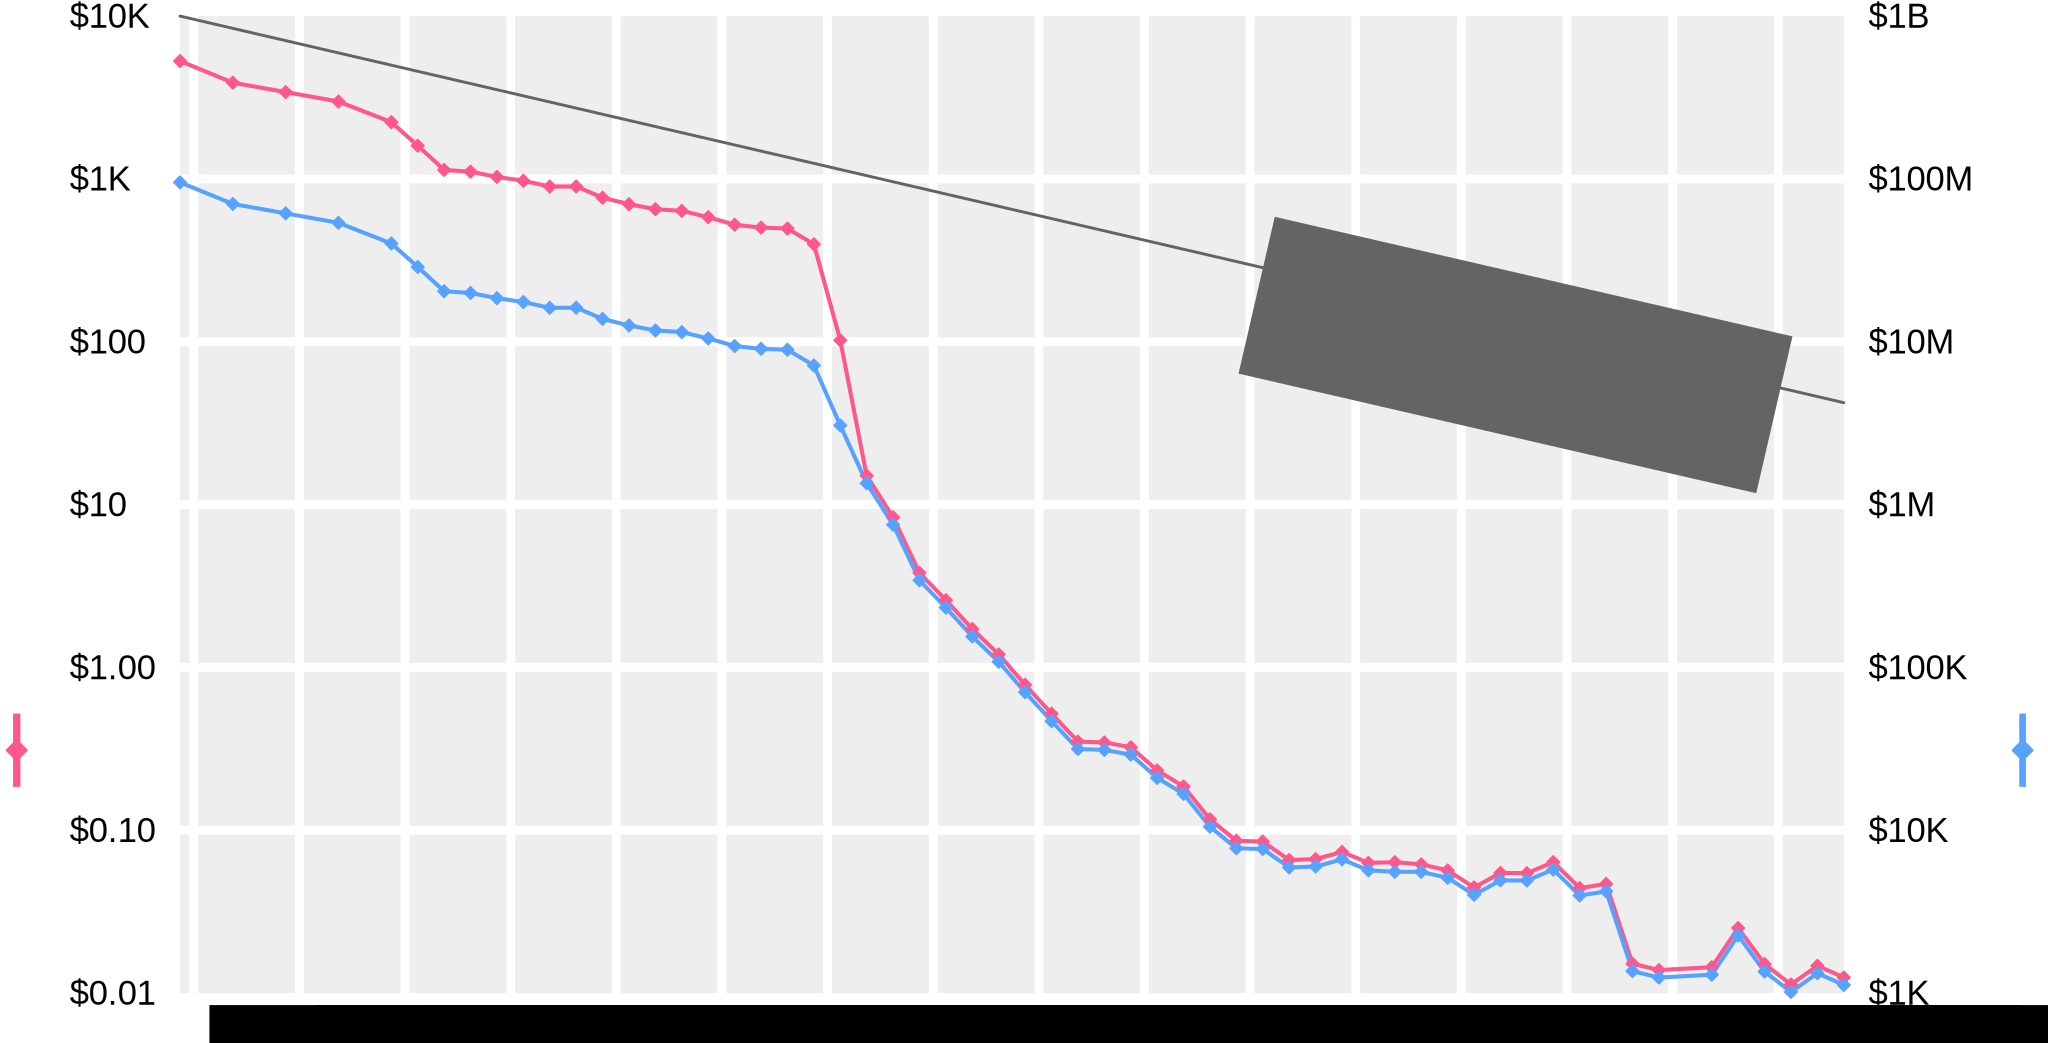
\includegraphics[width=\linewidth]{sequencing_costs.pdf}
    \caption[Sequencing costs per Mbp and per genome]{
        \textbf{Sequencing costs per Mbp and per genome.}
        The cost for DNA sequencing have decreased substantially in the past 15 years.
        The Figure shows the cost per mega-basepair (Mbp) of DNA (red line, left y-axis)
        as well as the cost per human-sized genome of $\approx$\,\num{3}\,Gbp (blue line, right y-axis).
        A basepair represents one character in the DNA.
        Note the logarithmic scaling of the y-axes.
        For comparison, Moore's law \cite{Moore1965} is shown.
        The particularly steep decrease in the beginning of 2008 is caused by
        the adoption of novel (next-generation) sequencing technologies in sequencing centers,
        see \secref{ch:Foundations:sec:SequenceAnalysis:sub:GenomeSequencing}.
        Source: Image based on data from \cite{Wetterstrand2018}.
%         \url{https://www.genome.gov/sequencingcosts/}
%         \url{https://www.genome.gov/sequencingcostsdata/}
    }
    \label{fig:sequencing_costs}
\end{figure}

In particular, these high-throughout technologies allow to directly sequence DNA contained in samples
that have been extracted from environments such as water, soil, or the human gut.
This results in so-called \emph{metagenomic} sequences,
i.e., anonymous DNA sequences from the (microbial) organisms that were present in the environmental sample.
A key question in the analysis of such data is to determine the evolutionary relationships of the sequences.
While these DNA sequences can hypothetically be used to infer phylogenetic trees from scratch,
this approach is limited by several theoretical and practical difficulties:
For instance, typical metagenomic samples contain too many, and too short, sequences
for a feasible and reliable tree inference.

One approach to tackle this issue is the so-called \emph{phylogenetic placement} \cite{Matsen2010,Berger2011},
of metagenomic sequences into a given phylogenetic tree (\secref{ch:Foundations:sec:PhylogeneticPlacement}).
Phylogenetic placement methods classify a set of \emph{query sequences}
into the context of known evolutionary relationships, provided in form of a \emph{reference tree}.
While this information already represents biological knowledge \emph{per se},
it can also be used for further downstream analyses \cite{Matsen2011a}.
The research in this field is however quite young and not many such analysis methods have been developed.

An important task prior to conducting phylogenetic placement of metagenomic sequences is to obtain a suitable
reference phylogenetic tree that captures the biological diversity of the species to be placed.
The assembly of a set of reference sequences from biological databases that can be used to infer such a tree
is typically a manual process, and hence both labor-intensive and potentially error-prone.
This might detain researchers from employing phylogenetic placement in the first place.

Furthermore, while the existing downstream methods for phylogenetic placement
(introduced in \secref{ch:Foundations:sec:PhylogeneticPlacement:sub:ExistingMethods})
allow for in-depth interpretation and visualization of the data,
they were not developed with a particular focus on large-scale studies comprising many thousand environmental samples.
For large datasets, these methods might provide too much detail,
making it hard to interpret results, to spot patterns and clusters in the data,
and to discover correlations with meta-data.

Lastly, the problem of scalability to large datasets does not only affect the methods themselves.
Because of the ever growing amount of sequence data,
scalability is becoming an issue for the software pipelines as well.
State-of-the-art phylogenetic placement implementations can place billions of sequences within a few hours \cite{Barbera2018}.
Methods for processing and analyzing the data, in particular phylogenetic placement data,
hence require efficient and scalable software implementations.

% ######################################################################################################################
%         Objective and Contribution
% ######################################################################################################################

\section{Objective and Contribution}
\label{ch:Introduction:sec:ObjectiveContribution}

in this thesis...

\chpref{ch:AutomaticTrees}

\chpref{ch:Visualization}

\chpref{ch:Clustering}

we developed methods for working with such data, and helped to conduct several empirical studies using established as well as our novel methods.

method papers (main contrib for this work, see next section)
phat \cite{Czech2018}
vis clust \cite{Czech2018a}



tree viz review \cite{Czech2017}



method and software dev:

salt \cite{Flouri2017}

unieuk \cite{Berney2017}

tree clustering workshop?

epa ng \cite{Barbera2018}

quartet score \cite{Zhou2017}

swarm code contrib \cite{Mahe2014,Mahe2015}

scrapp




data analysis:

1kite \cite{Misof2014}
\url{http://1kite.org}

neotrop \cite{Mahe2017}

microsopirida \cite{Bass2018a}

long reads (in prep)

dinos (in prep)




mention genesis and gappa, their implementation chapter in the appendix,
their paper?!
github links
\url{https://github.com/lczech/genesis}
\url{https://github.com/lczech/gappa}

genesis: implements some established methods, just way faster

mention  \url{http://github.com/lczech/placement-methods-paper} for the result files of two of the papers

full list of publications is available in \secref{ch:Publications}

% ######################################################################################################################
%         Structure and Overview
% ######################################################################################################################

\section{Structure and Overview}
\label{ch:Introduction:sec:StructureOverview}


\todo{check that the url and access date of all online sources are present in bibliography!}

% \todo{I used a few public domain images from wikipedia as sources, and modified them as needed. make sure that this is okay.}

\todo{search for all abbreviations used and add them to the acro list. also, check Pierre's MA, and Alexey's and Andre's Diss for needed acronyms!}
\todo{list of acronyms!} see andre, add MB/GB, PCA,
BV, TO, HMP, etc

\todo{unify table and figure caption capitalization}

\todo{more workflow flow charts?}

% ######################################################################################################################
%         Foundations
% ######################################################################################################################

\chapter{Foundations}
\label{ch:Foundations}

\paperbox{
    This chapter is partially based on the peer-reviewed publications:
}{\paperart \paperpppp}{
    \todo{
        \textbf{Contributions:} Lucas Czech... Pierre Barbera... Alexandros Stamatakis... and...
    }
}

\todo{In this chapter, we introduce\ldots}

% ######################################################################################################################
%         Evolution and Genetics
% ######################################################################################################################

\section{Evolution and Genetics}
\label{ch:Foundations:sec:EvolutionGenetics}

% Evolution is change in the heritable characteristics of biological populations over successive generations.
% \url{https://en.wikipedia.org/wiki/Evolution}
% the process by which new species or populations of living things develop from preexisting forms through successive generations
% \url{https://www.merriam-webster.com/dictionary/evolution}
% Evolution is a process of continuous branching and diversification from common trunks. This pattern of irreversible separation gives life's history its basic directionality. —Stephen Jay Gould
% \url{https://www.merriam-webster.com/dictionary/evolution}

% Evolution is the continuous process of diversification of biological populations through successive generations \cite{Hall2008}.

Life on Earth is at least 3.77 billion years old \cite{Dodd2017},
and is continuously evolving due to \emph{natural selection} \cite{Darwin1859}.
% Woah, I like that very first sentences. A very old and a very new publication, binding all of reasearch together...
Driven by \emph{variation}, biological populations diversify through successive generations,
leading to the origination of new species.
This continuous process is called \emph{evolution} \cite{Hall2008}.
Heritable characteristics are passed down from parent to offspring,
with occasional random mutations leading to variation.
Thus, some organisms are better adapted to their environment than others,
and have more reproductive success.
There is hence a natural selection for advantageous mutations,
which can then spread through generations.

% this process was not understood for a long time. static species?
% four driving forces of pop gen?

The characteristics and traits of an organism are carried by, and inherited via, \emph{deoxyribonucleic acid} (DNA).
DNA is the molecule that encodes the genetic information needed for the functioning of all living organisms.
It is structured in form of a double helix \cite{Watson1953},
and built from two strands of molecules called \emph{nucleotides}.
The nucleotides build the backbone of the double helix,
and connect the two strands via opposing pairs of \emph{nucleobases}, see \figref{fig:dna_nucleobases:sub:dna_helix}.
The redundant structure of pairs of nucleobases gives stability to the DNA molecule,
and also serves as a mechanism of error correction when reading the genetic information during cellular processes.
% both of which is important for the role of DNA for information storage.
In DNA, there are four distinct nucleobases:
adenine (\nucleobase{A}), cytosine (\nucleobase{C}), guanine (\nucleobase{G}), and thymine (\nucleobase{T}),
where \nucleobase{A} pairs with \nucleobase{T}, and \nucleobase{C} pairs with \nucleobase{G}, respectively,
as shown in \figref{fig:dna_nucleobases:sub:nucleobases}.

\begin{figure}[hpbt]
    \centering
    \includegraphics[width=.7\linewidth]{dna_nucleobases.pdf}
    \begin{subfigure}{0pt}
        \phantomcaption
        \label{fig:dna_nucleobases:sub:dna_helix}
    \end{subfigure}
    \begin{subfigure}{0pt}
        \phantomcaption
        \label{fig:dna_nucleobases:sub:nucleobases}
    \end{subfigure}
%     \begin{subfigure}{0pt}
%         \phantomcaption
%         \label{fig:dna_nucleobases:sub:transition_transversion}
%     \end{subfigure}
    \caption[DNA double helix and nucleobases]{
        \textbf{DNA double helix and nucleobases.}
        \subref{fig:dna_nucleobases:sub:dna_helix}
        The double helix structure of DNA, with the backbone in gray,
        connected by pairs of nucleobases.
        \subref{fig:dna_nucleobases:sub:nucleobases}
        The atomic structure of the four nucleobases, and their connection to each other.
%         Note that the diameter of the helix is about \SI{2}{\nano\meter}.
        Source and license: see \cite{Czech2018DNA},
        image derived from \cite{MesserWoland2006,Sponk2010,Yikrazuul2008a,Yikrazuul2008b}.
%         \\
%         Source: Image derived from \cite{Yikrazuul2008a,Yikrazuul2008b}.
%         Source: Image derived from \cite{Sponk2010}.
%         \subref{fig:dna_nucleobases:sub:transition_transversion}
%         Each nucleobase can mutate into any other in the course of evolution.
%         The two different types of mutation (transitions vs. transversions) are not equally likely,
%         due to physical properties of the nucleobases.
    }
    \label{fig:dna_nucleobases}
\end{figure}

% Transitions vs Transversions - not needed
% Over the course of evolutionary times, mutations in the DNA occur, mainly due to errors in the replication process.
% These mutations manifest in form of changed nucleobases.
% There are two types of mutations, \emph{transition} \emph{transversions}, which are not equally likely.
% \cite{Futuyma2013}
% \figref{fig:dna_nucleobases:sub:transition_transversion}

The sequence of nucleobases along the strands of DNA is what encodes the genetic instructions
used by all known living organisms.
Parts of the DNA encode for proteins,
which perform a plethora of different functions within organisms.
Proteins consist of long chains of amino acid residues, and
are assembled in a process called protein (bio)synthesis.
This is described by the central dogma of molecular biology \cite{Crick1958,Crick1970}:
First, DNA is \emph{transcribed} into the intermediary ribonucleic acid (RNA),
which is then \emph{translated} into the actual protein.

In each step of this process, the molecular alphabet used to encode information differs.
While DNA uses the four nucleobases as described above,
in RNA, the nucleobase uracil (\nucleobase{U}) is used instead of thymine (\nucleobase{T}).
Proteins on the other hand are (mostly) build from a set of \num{20} standard amino acids.
The set of rules used by the molecular machinery for translating nucleobases into amino acids
is called the \emph{genetic code}:
In a DNA sequence, three consecutive nucleobases are needed to encode one amino acid \cite{Shu2017}.

The entirety of the genetic material of an organism, that is, its complete DNA sequence, is called its \emph{genome}.
A \emph{gene} is a sequence which codes for a molecule that has a particular function, such as a protein \cite{Gericke2007}.
DNA and genes are the basic units of heredity.
They are what is varying across generations,
and what is selected for in the process of natural selection \cite{Dawkins1989}.
The study of genes, variation and heredity is called \emph{genetics} \cite{Griffiths2000}.

% ######################################################################################################################
%         Sequence Analysis
% ######################################################################################################################

\section{Sequence Analysis}
\label{ch:Foundations:sec:SequenceAnalysis}

All life on this planet is related to each other and descends from a common ancestor.
Still, it is remarkable that the basic molecular principles and mechanisms of life---%
DNA, amino acids, and the genetic code---are virtually identical for all living organisms.
This implies that by understanding and comparing the genetic information
encoded in the genetic sequences of different organisms,
one can understand the diversification patterns of evolution.

% ======================================================================================================================
%     Genome Sequencing
% ======================================================================================================================

\subsection{Genome Sequencing}
\label{ch:Foundations:sec:SequenceAnalysis:sub:GenomeSequencing}

Prior to analyzing the DNA of an organism, the physical order of nucleobases in the DNA molecule has to be determined.
That is, the DNA has to be ``read'' and stored in a human-accessible text format, typically a computer file.
This technical process is called DNA \emph{sequencing}.
% which can be understood as putting biomass into a blender and converting it into text files ;-)

For many decades, the main technique for this purpose was Sanger sequencing \cite{Sanger1975,Sanger1977}.
It is labor- and time-intensive, but through improvement and automation, costs were constantly reduced.
Eventually, this allowed for large-scale efforts, such as the Human Genome Project \cite{Venter2001},
which sequenced the whole human genome of more than three billion nucleobases.
Sanger sequencing allows to determine long parts of the sequence at once (> \num{500} nucleobases),
which then have to be assembled to build the final sequence.

In the last decades, a variety of novel high-throughput DNA sequencing technologiesß
have been developed \cite{Pettersson2009,Reuter2015,Goodwin2016}.
In particular, \emph{Next Generation Sequencing} (NGS) \cite{Logares2012,Mardis2013}
has revolutionized biology by transforming it into a data-driven and compute-intense discipline \citep{Escobar-Zepeda2015}.
The costs of these technologies are decreasing faster than Moore's law \cite{Wetterstrand2018}.
This leads to a ``tsunami'' of sequence data,
which poses a challenge for computational methods working with these data.
Compared to Sanger sequencing, NGS technologies are generally cheaper and faster \cite{Voelkerding2009,Metzker2010},
but come at the price of introducing more errors in the sequence output,
or only being able to determine shorter parts of the sequence at once
-- both of which constitute a challenge for the subsequent assembly of the final sequence.

The result of DNA sequencing is a textual representation of the order of nucleobases.
Although this representation ignores the physical and chemical properties of the respective molecules,
it is helpful in many applications, and allows to leverage existing algorithms.
Each contiguous sequence coming from the sequencing machine is called a \emph{read}.
Because of the pairing of nucleobases,
both DNA strands can be sequenced, which provides a means of error correction.
Such data are typically stored in the \fileformat{fastq} file format \citep{Cock2009}.
These so-called paired-end reads are then merged to form a final sequence representation of one strand
% cite \toolname{PEAR} \cite{Zhang2014} ?
-- that is, a sequence of the characters \nucleobase{A}, \nucleobase{C}, \nucleobase{G}, and \nucleobase{T}.
These data are stored in formats such as the \fileformat{fasta} file format \citep{Pearson1988}.
Due to the pairing of nucleobases,
the length of a DNA sequence is measured in \emph{base pairs} (abbreviated \si{\basepair}):
\SI{1}{\basepair} represents one character in the file.
These files are then the input for computational methods for working with DNA sequences.

% Not needed right now:
% Because of the universal genetic code of translating DNA to amino acids,
% it is also possible to store the amino acid sequence instead of the nucleobase sequence.

% ======================================================================================================================
%     Metagenomics
% ======================================================================================================================

\subsection{Metagenomics}
\label{ch:Foundations:sec:SequenceAnalysis:sub:Metagenomics}

Sanger sequencing requires careful preparation of the genetic material,
and is thus best used for sequencing single organisms.
There are however many (microbial) organisms that cannot be cultured in a Petri dish,
and are hence hard to sequence with this technique.
Apart from being cheaper, Next Generation Sequencing machines however ``digest'' all genetic material presented to them.
They thus allow for studying microbial samples
directly extracted from their environment \citep{Morgan2010,Edwards2013,Sunagawa2013a}.
This enables to study environments such as
water \cite{Karsenti2011,Giner2016,Gran-Stadniczenko2017},
soil \cite{Dupont2016,Mahe2017},
the human body \cite{Huttenhower2012,Methe2012,Matsen2015,Wang2015},
and many others.
Each sample from such an environment then represents a geographical location, a body site, a point in time, etc.
% These studies yield a large set of short anonymous DNA reads for each sample.
% The DNA reads obtained from sequencing a sample represent all organisms present in the sample;
The DNA of all organisms being present in a sample is sequenced,
resulting in a large number of reads per sample.
These reads are anonymous, as it is unclear to which organism they originally belonged.
The study of these data, that is, genetic material from environmental samples, is called \emph{metagenomics} \cite{Oulas2015}.

% \paragraph{Key Tasks}
% \label{ch:Foundations:sec:SequenceAnalysis:sub:Metagenomics:par:KeyTasks}

% A first step is often to generate a genetic profile of the environment,
% that is, to estimate the diversity of the organisms in the sample.
A first step in metagenomic studies is often to characterize the reads obtained from an environment
in terms of \emph{reference sequences} of known species.
Reads that are similar to (parts of) reference sequences can be assigned to them,
while reads with low similarity to known sequences might indicate novel, undescribed species \cite{Temperton2012}.
Key tasks in metagenomic studies are the identification and classification of the anonymous reads (``Who is there?''),
and their functional annotation (``What are they doing?'') \cite{Desai2012}.
Both are introduced in the following.

% The following paragraph is not totally needed, as we are not doing functional analysis.
% However, it introduces many other terms alongside, which is useful later on.
Functional annotation \cite{Stein2001} is the prediction of gene functions of the reads,
and the inference of metabolic capacity of microbial communities \cite{Brown2017}.
As the proteins that are needed in the pathways of such functions can be encoded by genes across the genome,
whole-genome sequencing is necessary to capture all genes of interest.
For example, in shotgun sequencing \cite{Staden1979,Anderson1981},
the DNA is fragmented into small pieces within the size range that the used sequencing technology can handle,
typically a few hundred \si{\basepair} long.
This allows to sequence all genetic material contained in a sample.
Thus, the resulting reads originate from different parts of the genomes of their organisms,
which can then be functionally annotated \cite{Glass2010}.
This however necessitates to use whole-genome reference sequences
in order to be able to assign reads to known species and functions.
Typical databases of reference sequences however
lack many of the protein sequences from the microbial species present in a sample,
mostly because of organisms that cannot be cultured \cite{Brown2017}.

For the task of identification and classification of reads however, whole genome references are not needed.
Instead, specific \emph{marker genes} can be used,
which are regions of genes that are particularly suited for delineating between different species \cite{Ren2016}.
% highly conserved, that is, slowly changing over evolutionary times.
% but certain parts are radpidly evolung (hyper variable) withing the region, which is good for delineation.
% typically, this is general basic cell functionen stuff, which is needed by many forms of live.
% eg cell division, ssu... mitochondrial dna, etc
The method of using marker genes to identify species is called \emph{DNA barcoding} \cite{Hebert2003,Savolainen2005,Deiner2017b}.
The choice of genes to use as marker is important, and depends on the types of organisms to be studied.
The used marker genes should ideally be present in all of the organisms of interest,
short enough to be sequenced with current technology,
and have enough variation between species to distinguish between them,
but have low variation within species \cite{Kress2008}.

% \paragraph{Typical Processing}
% \label{ch:Foundations:sec:SequenceAnalysis:sub:Metagenomics:par:TypicalProcessing}

In many metagenomic studies of \taxonname{bacteria} and \taxonname{eukaryota},
the 16S \cite{Weisburg1991} and 18S \cite{Meyer2010} rRNA regions are used as marker genes,
respectively \cite{Woese1977,Woese1990}.
These regions belong to the small subunit (SSU) of the ribosomal ribonucleic acid (rRNA),
which is an essential component of the ribosome.
The ribosome is a molecular machinery that is responsible for protein synthesis (translation) in all living organisms.
% and are thus present in virtually all \taxonname{bacteria} and \taxonname{eukaryota}.
Often, prior to sequencing, these regions are amplified by many orders of magnitude,
using polymerase chain reaction (PCR) to create copies of these regions \cite{Bartlett2003}.
The resulting reads are then de-replicated again, which results in sequences called \emph{amplicons}.
While the PCR amplification process is known to introduce bias \cite{Logares2014,Brown2017},
this inexpensive method is commonly used in practice, particularly for the 16S and 18S rDNA regions.
A recent alternative to using PCR for obtaining reads from these regions are \textsubscript{mi}tags \citep{Logares2014}.
In this approach, shotgun sequencing is used to get reads from the whole genomes of the organisms in a sample.
These reads are then filtered to only contain reads from the 16S region (for \taxonname{bacteria}),
which capture the diversity of the sample without bias.

Because of the ubiquity of the 16S and 18S rDNA regions in organisms and, consequently, in sequencing studies,
many databases provide reference sequences for these marker regions.
The reads or amplicons obtained from an environmental sample can then be employed
to estimate the microbial diversity of the organisms in the sample by comparison against known species.

% ======================================================================================================================
%     Sequence Alignments
% ======================================================================================================================

\subsection{Sequence Alignment}
\label{ch:Foundations:sec:SequenceAnalysis:sub:SequenceAlignment}

Organisms that evolved from a (not too distant) common ancestor share genetic information.
Regions of their DNA that have a shared ancestry are called \emph{homologous} regions \cite{Koonin2005}.
This homology is typically inferred from sequence similarity. %, that is, by comparison of the sequences.
However, due to mutations, differences in the sequences can occur.
There are three main types of sequence mutations that can occur in evolution:
a \emph{substitution} is the exchange of a nucleobase for another;
a \emph{insertion} adds one or more extra nucleotides into the sequence;
a \emph{deletion} removes one or more nucleotides from the sequence.
The latter two types of mutations change the length of the sequence;
a mutation that is either one of them is called an \emph{indel}.

Because of indels, sequences have to be aligned to each other in order to compare their homologous regions.
That is, gap characters (\nucleobase{-}) have to be added to the sequences
such that homologous characters in the sequence get aligned.
This results in an $n \times m$ matrix,
where $n$ is the number of sequences (rows),
and $m$ is the number of homologous characters (columns), called \emph{sites}.
This matrix is called a \emph{multiple sequence alignment} (MSA), or simply an \emph{alignment}.
\figref{fig:msa} shows an example of the alignment process and the resulting MSA.

\begin{figure}[hpbt]
    \centering
%     \vspace*{0.5em}
    \includegraphics[width=.9\linewidth]{msa.pdf}
    \caption[Multiple Sequence Alignment]{
        \textbf{Multiple Sequence Alignment.}
        The left hand side shows a set of six sequences.
        Using an alignment algorithm, gaps are inserted into these sequences at presumed indel positions.
        The right hand side shows the result of this process,
        where homologous characters at the sites of the multiple sequence alignment (MSA) are aligned to each other.
        Below the MSA, the majority rule consensus sequence is shown,
        see \secref{ch:Foundations:sec:SequenceAnalysis:sub:ConsensusSequences}.
    }
    \label{fig:msa}
\end{figure}

Sequence alignment can be understood as an optimization problem under a given optimality criterion.
On the one hand, \emph{global alignments} attempt to align every character in every sequence,
which is most useful for similar sequences of roughly equal size.
For example, the Needleman-Wunsch algorithm \cite{Needleman1970} is a general global alignment technique
based on dynamic programming.
On the other hand, \emph{local alignments} are better suited for dissimilar sequences
which might contain similar regions within a larger sequence context.
The Smith-Waterman algorithm \cite{Smith1981} is a general local alignment technique
using the same dynamic programming scheme,
which additionally allows to start and end at any place in the sequence.
As both algorithms have their particular use cases \cite{Polyanovsky2011},
hybrid methods have also been developed \cite{Brudno2003}.
Furthermore, heuristic approaches such as \toolname{BLAST} \cite{Altschul1990} and
\toolname{USEARCH} \cite{Edgar2010} can calculate millions of near-optimal alignments in reasonable time.

These algorithms are efficient for the pairwise alignment of two sequences.
Calculating an MSA however has been shown to be NP-hard \cite{Wang1994,Just2001}.
Thus, for most empirical data sets, other approaches and heuristics are needed \cite{Thompson2011}.
Tools such as \toolname{CLUSTAL} \cite{Higgins1988}, \toolname{MUSCLE} \cite{Edgar2004}, and \toolname{MAFFT} \cite{Katoh2002}
can calculate near-optimal multiple sequence alignments for many thousands of sequences.

A special use case for aligning sequences arises in metagenomic studies,
where environmental sequences are often compared to a set of known reference sequences.
In these studies, one often first calculates an MSA of the reference sequences,
and then successively aligns the environmental sequences against this MSA.
This is because calculating an MSA for millions or billions of sequences from scratch is too expensive even for modern tools.
Hence, specialized algorithms for this use case have been developed,
such as \toolname{PaPaRa} \citep{Berger2011a,Berger2012} and
\toolname{hmmalign}, which is a subprogram of the \toolname{HMMER} suite \citep{Eddy1998,Eddy2009}.

% ======================================================================================================================
%     Consensus Sequences
% ======================================================================================================================

\subsection{Consensus Sequences}
\label{ch:Foundations:sec:SequenceAnalysis:sub:ConsensusSequences}

When working with a number of related but not identical sequences,
it is often convenient to ``summarize'' homologous characters in form of a \emph{consensus sequence}.
Such a sequence is typically calculated based on the relative frequencies of the characters per alignment site.
It then represents typical features and motifs of the input set of sequences.

The most straight forward method is to construct \emph{majority rule consensus} sequences \citep{May1952,Day1992a},
where each site is represented by the most frequent character at that site.
\figref{fig:msa} shows an example below the MSA on the right hand side.
In order to also include information from the less frequent characters at a site in the consensus sequence,
\emph{ambiguity characters} can be used \cite{IUPAC1970}.
They allow to denote multiple alternative nucleobases as a single character.
For example, if the nucleobases \nucleobase{A} and \nucleobase{G} are similarly frequent at a site,
this site is represented by the ambiguity character \nucleobase{R}.
See \tabref{tab:AmbiguityCharacters} for the full list of character representations.

Using ambiguity characters allows for more involved consensus methods.
For example, \emph{threshold consensus} sequences \citep{Day1992a,Day1992} include the most frequent characters
that are needed to achieve some given frequency threshold per site,
and represent these characters by their ambiguity character.
Furthermore, many methods based on fixed thresholds have been proposed,
such as Cavener's method \citep{Cavener1987,Cavener1991a};
see \cite{Day1992a} for a critical comparison.

It is theoretically also possible to directly use the relative frequencies of characters per site
in the mathematical frameworks of many downstream analysis methods.
This would allow to leverage all of the information contained in the input set of sequences.
However, to our knowledge, there is no convention or file format to store such information,
and consequently, no way of forwarding this information to the respective tools.

% ######################################################################################################################
%         Tree of Life
% ######################################################################################################################

\section{The Tree of Life}
\label{ch:Foundations:sec:TreeOfLife}

The shared evolutionary history of life gives rise to a branching pattern,
where new \emph{lineages} split from a common ancestor.
This branching pattern forms a tree-like structure,
which classifies organisms in a hierarchy based on common descent.

While this \emph{tree of life} is an expedient and, hence, pervasive model \cite{Mindell2013},
it ignores certain biological and evolutionary events.
A strict hierarchy does not allow for reticulate events,
such as hybridization \cite{Maddison1997a}, genetic recombination \cite{Hein1993},
or horizontal gene transfer \cite{Ochman2000,DunningHotopp2011,Robinson2013}.
Although approaches such as networks have been proposed to model these events \cite{Huson2011a},
the simplicity of a hierarchy or tree structure still has proven
to be useful in classifying and naming organisms, and understanding their evolutionary relationships.

% not considering lat gene tranfs, there is only one ``true'' tree of life.

% For the \taxonname{eukaryota}, the tree model is still considered valid.
% However, \taxonname{bacteria} have the ability of horizontal gene transfer,
% where genetic information is transferred between unrelated organisms.

% biology is messy: https://www.ncbi.nlm.nih.gov/pubmed/20852602

% ======================================================================================================================
%     Taxonomy and Nomenclature
% ======================================================================================================================

\subsection{Taxonomy and Nomenclature}
\label{ch:Foundations:sec:TreeOfLife:sub:TaxonomyNomenclature}

Early attempts at classifying organisms date back to the Greek philosopher Aristotle,
who used observable attributes to divide living things into groups \cite{Leroi2014}.
This approach as well as the efforts of later centuries were non-uniform and inconsistent.
The basis for the modern system of classification was established
by Swedish botanist Carl Linnaeus in the mid-18th century \cite{Donk1957}.
He proposed a \emph{nomenclature}, that is, a naming system for organisms,
as well as a \emph{taxonomy}, that is, a rank-based classification of organisms \cite{Linnaeus1735,Linnaeus1753}.

A taxonomic group of organisms is called a \emph{taxon} (plural: \emph{taxa}).
Each taxon is associated with a \emph{taxonomic rank}, which can subsume other ranks,
thus forming a hierarchy of higher and lower ranks.
A taxonomic rank represents the relative level of a group of organisms in the taxonomy.
The principal ranks in modern use are \taxonname{domain}, \taxonname{kingdom}, \taxonname{phylum}, \taxonname{class},
\taxonname{order}, \taxonname{family}, \taxonname{genus}, and \taxonname{species},
see \figref{fig:taxonomic_ranks}.
If needed, further ranks can be included in between (such as \emph{sub-genus}),
or more refined lower levels be added (such as \emph{strain}, which is a further distinction within a species).

\begin{figure}[hpbt]
    \centering
%     \vspace*{0.5em}
    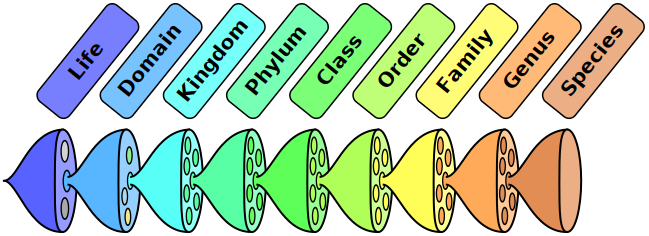
\includegraphics[width=.85\linewidth]{taxonomic_ranks.pdf}
    \caption[Biological classification into taxonomic ranks]{
        \textbf{Biological classification into taxonomic ranks.}
        The figure depicts a typical set of nested taxonomic ranks \cite{Woese1990},
        which form a hierarchy with increasingly deeper levels towards the right.
%         The taxonomic ranks shown here follow the three-domain system \cite{Woese1990}.
%         which classifies cellular life into the domains \taxonname{archaea}, \taxonname{eukaryota}, and \taxonname{bacteria}.
%         The deeper levels towards the right form a hierarchy of nested taxonomic ranks.
        Source: Image derived from \cite{Halasz2007}.
    }
    \label{fig:taxonomic_ranks}
\end{figure}

In order to scientifically name the groups of organisms (taxa) in a taxonomy,
the \emph{binomial nomenclature} as introduced by Linnaeus is still prevalent to this day.
It uses two terms, often of Latin origin,
which respectively specify the taxonomic ranks \emph{genus} and \emph{species} that an organism belongs to,
for example \taxonname{Homo sapiens}.

While early classifications used \emph{phenotypes}, that is, observable characteristics or traits of organisms,
modern approaches to taxonomy take genetic information into account \cite{Mayr2002}.
For example, the three-domain system \cite{Woese1977,Woese1990} resolves the oldest evolutionary relationships,
that is, the highest taxonomic levels, based on 16S rRNA data.
Although this classification has been challenged \cite{Gupta1998,Mayr1998,Cavalier-Smith2002}, it is widely used.
It divides cellular life forms into the three domains \taxonname{bacteria}, \taxonname{archaea}, and \taxonname{eukaryota};
the latter is further separated into kingdoms,
which include the kingdoms \taxonname{fungi}, \taxonname{plants}, and \taxonname{animals}.

% Archaea, Domain (and Kingdom)
% Eukarya, Domain
% Protista, Kingdom
% Fungi, Kingdom
% Animalia, Kingdom
% Plantae, Kingdom
% Bacteria, Domain (and Kingdom)

% ======================================================================================================================
%     Phylogenetic Trees
% ======================================================================================================================

\subsection{Phylogenetic Trees}
\label{ch:Foundations:sec:TreeOfLife:sub:PhylogeneticTrees}

The classification of organisms into a taxonomy is based on (subjective) dissimilarity and thus arbitrary:
The number of organisms that are grouped into a taxon at a given rank can vary,
and the separation into discrete ranks does not reflect the gradual nature of evolution \cite{Gingerich1987}.
A more involved approach that can resolve these issues is \emph{phylogenetics},
which is the study of the evolutionary history and relationships of biological entities (individuals, species, populations).

The evolutionary relationships of such entities are called their \emph{phylogeny}.
As the true phylogeny of a set of taxa is unknowable,
it has to be inferred from data that is available.
A phylogenetic analysis uses inference methods that evaluate observed heritable traits
in order to resolve the phylogeny under a given model of evolution of these traits.
While phenotypes can be used, modern phylogenetic inference is mostly based on DNA data.
The result of a phylogenetic analysis is a \emph{phylogenetic tree},
also called an \emph{evolutionary tree}, or---synonymously---a \emph{phylogeny}.
\figref{fig:tree_of_life} shows two examples of phylogenetic trees.

\begin{figure}[hpbt]
    \centering
    
\includegraphics[width=\linewidth]{tree_of_life.pdf}
    \begin{subfigure}{0pt}
        \phantomcaption
        \label{fig:tree_of_life:sub:darwin}
    \end{subfigure}
    \begin{subfigure}{0pt}
        \phantomcaption
        \label{fig:tree_of_life:sub:woese}
    \end{subfigure}
    \caption[Exemplary phylogenetic trees]{
        \textbf{Exemplary phylogenetic trees.}
        \subref{fig:tree_of_life:sub:darwin}
        In 1837, Charles Darwin sketched his first evolutionary tree below the words ``I think''
        in his notebook on ``Transmutation of Species''.
        Source: Image derived from \cite{DarwinTreeOfLife1837}.
%         \\
        \subref{fig:tree_of_life:sub:woese}
        A modern phylogenetic tree showing the three-domain system \cite{Woese1977,Woese1990},
        which emphasizes the separation of \taxonname{bacteria}, \taxonname{archaea}, and \taxonname{eukaryota}
        based on 16S rRNA genes.
        The black branch at the bottom represents the speculative last universal common ancestor of all living organisms.
        Source: Image derived from \cite{WoeseTreeOfLife2006}.
    }
    \label{fig:tree_of_life}
\end{figure}

\paragraph{Properties of Trees}
\label{ch:Foundations:sec:TreeOfLife:sub:PhylogeneticTrees:par:TreeProperties}

The leaf nodes, or \emph{tips}, of the tree represent living (\emph{extant}) biological entities
such as species, strains, individual organisms, or even cells of a multicellular organism.
Thus, the tips are often referred to as the \emph{taxa} of the tree,
which is meant as a generic term that includes all the above entities.
The tips are often named according to the entities they represent (e.\,g., species names);
such a tree is called a \emph{labeled} tree.
The inner nodes on the other hand are usually anonymous and
represent speciation events, where two novel lineages arose from a putative common ancestor.
The branching pattern of a phylogenetic tree thus reveals the evolutionary history of its taxa.

The edges of the tree, also called its \emph{branches}, can have associated \emph{branch lengths},
which represent the evolutionary time between the two adjacent nodes,
for example, measured as the average change in nucleobases between their respective sequences.
The unique path between any two nodes thus can be interpreted
as a measure of evolutionary relatedness of the taxa represented by the nodes.

A phylogenetic tree is \emph{rooted}
if it is a directed tree that has a unique \emph{root node},
which corresponds to the putative common ancestor of the other nodes in the tree.
See \figref{fig:tree_of_life:sub:woese} for an example.
As evolution is a processes that happens over time,
from a biological point of view, every tree has a root.
However, most models of DNA evolution are time-reversible,
meaning that the direction of change in the sequences cannot be inferred from the data under such models,
see \secref{ch:Foundations:sec:MLTreeInference:sub:ModelsOfSeqEvol} for details.
Thus, tree inference methods can also yield \emph{unrooted} trees without direction and without a root node.
In these methods, for computational reasons, often a \emph{virtual root} is used,
which is a hypothetical additional node placed on a branch of the tree.
For tasks such as traversing a tree, but also in order to store a tree in a file,
unrooted trees usually have a distinguished, but arbitrary, ``starting'' node called a \emph{top-level trifurcation}.
An unrooted tree can be rooted a posteriori, for example by using an \emph{outgroup} of taxa
that are closely related to the group of taxa of interest (the \emph{ingroup}), but not part of it.
Then, a root node can be placed on the branch that separates the outgroup from the ingroup.

An inner node that has exactly three neighboring nodes is called a \emph{bifurcation} or a \emph{bifurcating} node.
In rooted trees, these neighbors are the the parent and the two children of a node, hence the name.
An inner node with more neighbors is called a \emph{multifurcation} or a \emph{multifurcating} node.
This naming also applies to the whole tree:
A tree, where each inner node (with the exception of the root node in a rooted tree) is bifurcating,
is also called a bifurcating tree.
Otherwise (if there is at least one multifurcating node), it is a multifurcating tree.
Note that in evolution, an actual multifurcation event is highly unlikely,
as it corresponds to the simultaneous formation of more than two new lineages from a single ancestral lineage.
Multifurcating trees are for example used when relationships cannot be properly resolved from the existing data,
or to summarize a set of otherwise contradicting trees.

Each edge of the tree induces a \emph{bipartition} or \emph{split} of the taxa of the tree into two groups,
one on each side of the edge.
A set of taxa is \emph{monophyletic},
if there is a bipartition of the tree that splits these taxa from all other taxa of the tree.
In a rooted tree, the node at the end of that edge is then the putative common ancestor of these taxa.
Furthermore, a monophyletic set of taxa is called a \emph{clade} of the tree;
in other words, a clade is a subtree that is separated from the rest of the tree by one edge.
For example, the taxa {\sffamily A}, {\sffamily B}, and {\sffamily C} in \figref{fig:tree_vis_options} are monophyletic---%
that is, they form a clade of the tree.
Lastly, a non-monophyletic set of taxa is \emph{paraphyletic}.

\paragraph{Practical Aspects of Trees}
\label{ch:Foundations:sec:TreeOfLife:sub:PhylogeneticTrees:par:PracticalAspects}

While the topology of the tree is what models the evolutionary relationships,
there are several ways of visualizing or drawing that information.
\figref{fig:tree_vis_options} shows some examples, which all visualize the same topology (except for the rooting).
The figure also summarizes some of the terms and concepts introduced above.
Different drawing styles each have their advantages.
For example, in a rectangular tree (\figref{fig:tree_vis_options:sub:rectangular}),
branch lengths are easier to read and compare,
while a circular tree (\figref{fig:tree_vis_options:sub:circular}) can fit more taxa in the same drawing area.

\begin{figure}[hpbt]
    \centering
    \includegraphics[width=\linewidth]{tree_vis_options.pdf}
    \begin{subfigure}{0pt}
        \phantomcaption
        \label{fig:tree_vis_options:sub:unrooted}
    \end{subfigure}
    \begin{subfigure}{0pt}
        \phantomcaption
        \label{fig:tree_vis_options:sub:rectangular}
    \end{subfigure}
    \begin{subfigure}{0pt}
        \phantomcaption
        \label{fig:tree_vis_options:sub:circular}
    \end{subfigure}
    \caption[Types of phylogenetic trees]{
        \textbf{Types of phylogenetic trees.}
        Here, we show three different types of labeled, bifurcating trees.
        Tip nodes are marked with black dots, inner nodes with white dots,
        and the top-level trifurcation or root node with a larger green dot.
        \subref{fig:tree_vis_options:sub:unrooted}
        An unrooted tree with five taxa. One node is arbitrarily selected as top-level trifurcation.
        \subref{fig:tree_vis_options:sub:rectangular}
        The same tree topology,
        but rooted on the inner branch that splits the taxa {\sffamily D} and {\sffamily E} from the other taxa.
        The tree is drawn in rectangular style,
        where vertical lines correspond to branch lengths.
        The horizontal lines are simply used to distribute the taxa, and have no biological interpretation.
        \subref{fig:tree_vis_options:sub:circular}
        The same tree again, but this time drawn in circular style.
        Here, radial lines correspond to branch lengths, while arcs only serve drawing purposes.
    }
    \label{fig:tree_vis_options}
\end{figure}

Taxonomy and phylogeny serve a related, but different purpose:
While the former is a system of classification,
the latter reveals evolutionary history.
However, there is a correspondence between a taxonomy and a rooted phylogeny:
Inner nodes of the tree constitute older evolutionary relationships,
which are represented by the higher ranks of the taxonomy.
\figref{fig:tree_of_life:sub:woese} shows such a correspondence for the three domains of life.
It is however possible that the taxa at one rank of the taxonomy are not monophyletic in the tree.
In this case, the two are \emph{incongruent}.

% particularly considering that the genes might evolve differently from the species or from what the taxonomy says

The most common file format for storing phylogenetic trees is the \fileformat{Newick} format \cite{Archie1986},
which uses parentheses and commas to specify the nesting structure of the tree,
and allows to store node labels and branch lengths.
The \fileformat{NEXUS} format \cite{Maddison1997} is a container format for biological data,
and internally also relies on the \fileformat{Newick} format for storing trees.
Furthermore, the \fileformat{phyloXML} format \cite{Han2009} is an \fileformat{XML} based format
that allows to store arbitrary data at the nodes and edges of the tree.
% This is particularly useful for annotating the tree with additional data.

% ======================================================================================================================
%         Tree Inference
% ======================================================================================================================

\subsection{Tree Inference}
\label{ch:Foundations:sec:TreeOfLife:sub:TreeInference}

A phylogeny can be inferred from data that has per-taxon traits which are homologous,
that is, which have evolved from the same traits in the common ancestor and are thus comparable \cite{Felsenstein2004,Yang2006}.
While historically these traits were mostly phenotypes (bone shapes and sizes, metabolism, etc.),
the focus has since shifted towards molecular data such as DNA and amino acid sequences,
as their \emph{phylogenetic signal} is generally more abundant and less biased \cite{Hillis2000}.
Most often, a multiple sequence alignment is used,
whose homologous sites represent the traits of the taxa.
To determine the degree of relatedness between taxa, mathematical models of trait evolution are employed.

% Searching the tree space
The general concept of tree inference is then to put closely related taxa close to each other in the phylogeny.
Hence, a tree inference can be thought of as an optimization problem,
which searches for the best tree given an optimality criterion.
However, the space of all possible tree topologies is too large for an exhaustive brute-force search
for virtually all empirical datasets.
For a given number of taxa $n$, the number of distinct tree topologies N is given as
$N(n) = \prod_{\,i=3}^{\,n} ~(2i - 5)$,
which grows over-exponentially fast \cite{Felsenstein2004}.
There are thus different approaches and heuristics to conduct tree search.

% Methods overview
Distance based methods such as \emph{Unweighted Pair Group Method with Arithmetic Mean} (UPGMA) \cite{Sokal1958}
and \emph{Neighbor Joining} \cite{Saitou1987}
use a pairwise distance matrix between sequences, and thus do not necessarily need an alignment.
\emph{Maximum Parsimony} \cite{Sankoff1975} uses an optimality criterion that is based on Occam's razor,
that is, it yields the tree that explains the observed tip sequences (taxa)
with the minimal number of substitutions (mutations).
The \emph{Maximum Likelihood} (ML) method \cite{Felsenstein1981} employs statistical techniques
in order to evaluate the probability of a given phylogenetic tree with respect to a given alignment,
and successively search the tree space for the most likely tree, see \secref{ch:Foundations:sec:MLTreeInference}.
Furthermore, \emph{Bayesian Inference} also relies on the evaluation of tree probability \cite{Yang2006},
and uses Bayes' theorem to calculate the posterior distribution of the relevant evolutionary processes;
it thus can incorporate prior empirical knowledge into the process.

Typical software tools for inferring ML trees include \toolname{IQ-TREE} \cite{Nguyen2015a},
\toolname{FastTree} \cite{Price2010}, and \toolname{RAxML} \cite{Stamatakis2014},
while Bayesian inference can for example be conduced using tools such as \toolname{BEAST} \cite{Suchard2018}
or \toolname{MrBayes} \cite{Ronquist2003}.

% ######################################################################################################################
%     Maximum Likelihood Tree Inference
% ######################################################################################################################

\section{Maximum Likelihood Tree Inference}
\label{ch:Foundations:sec:MLTreeInference}

In the context of this work, we are mostly interested in Maximum Likelihood (ML) tree inference.
It uses a probabilistic framework in which the (phylogenetic) likelihood

\begin{equation}
    \label{ch:Foundations:sec:MLTreeInference:eq:likelihood}
    \mathcal{L}(~ \mbox{MSA} ~|~ T, \bar{b}, M, \bar{\theta} ~)
\end{equation}

is evaluated that an observed MSA is the outcome of an evolutionary history described by a phylogenetic tree
with topology $T$ and branch lengths $\bar{b}$, under a given model of trait evolution $M$ with parameters $\bar{\theta}$.
For a fixed model $M$ (see \secref{ch:Foundations:sec:MLTreeInference:sub:ModelsOfSeqEvol}),
the likelihood can be expressed as a function of $T$, $\bar{b}$ and $\bar{\theta}$,
which is known as the \emph{phylogenetic likelihood function} (PLF).

% ======================================================================================================================
%     Tree Search
% ======================================================================================================================

\subsection{Tree Search}
\label{ch:Foundations:sec:MLTreeInference:sub:TreeSearch}

By maximizing the PLF using maximum likelihood estimation,
the parameter values (including tree topology) are found which best explain the observed data.
This process is called \emph{tree search}.
Typically, the estimates are obtained in an iterative process,
which alternates between two phases until a (potentially local) optimum is found:

\begin{enumerate}
    \item Optimizing the tree topology $T$, given the branch lengths $\bar{b}$ and the model parameters $\bar{\theta}$.
    \item Optimizing the branch lengths of the given tree topology, as well as the model parameters.
\end{enumerate}

% Optimizing the topology:
Finding the most likely tree topology is a discrete optimization problem,
which has been shown to be NP-hard under the ML criterion \cite{Chor2005}.
Furthermore, the evaluation of the PLF is computationally expensive,
as it involves many floating point operations, see \secref{ch:Foundations:sec:MLTreeInference:sub:LikelihoodComputation}.
A general heuristic for the tree search that avoids an exhaustive evaluation of the tree space is thus as follows.
First, a starting tree is generated, either randomly, or using methods such as Neighbor Joining or Maximum Parsimony.
Then, the likelihood of the tree is successively improved
by applying topological rearrangements (\emph{moves}) of its taxa and clades.
For instance, in \emph{greedy hill-climbing} \cite{Stamatakis2014}, only those moves are applied (\emph{accepted})
that immediately improve the PLF.

%Optimizing branch lengths and model parameters:
For a fixed tree topology $T$, the maximum likelihood estimates
of the branch lengths $\bar{b}$ and the model parameters $\bar{\theta}$
are usually obtained with general-purpose numerical optimization methods.
Since the derivatives of the PLF can be easily computed,
the Newton-Raphson method \cite{Ypma1995} is often used for optimizing the branch lengths,
see \secref{ch:Foundations:sec:MLTreeInference:sub:BLO}.
Model parameters are commonly optimized with Brent's method \cite{Brent1971}
or with the Broyden-Fletcher-Goldfarb-Shanno (BFGS) algorithm \cite{Fletcher1987}.

% ======================================================================================================================
%     Models of Molecular Sequence Evolution
% ======================================================================================================================

\subsection{Models of Molecular Sequence Evolution}
\label{ch:Foundations:sec:MLTreeInference:sub:ModelsOfSeqEvol}

So far, we assumed to have a model $M$ for describing the evolution of the traits that are used for inferring the tree.
For sequence data, such a model yields an estimate of the evolutionary distance between the sequences of different taxa.
Because the inference assumes homologous traits,
the only mutations that are typically considered in aligned sequences are substitutions.
% Gap characters in the MSA (see \secref{ch:Foundations:sec:SequenceAnalysis:sub:SequenceAlignment}),
% which account for indels, can then be thought of as another type of substitution.

\paragraph{Markov Chain Model}
\label{ch:Foundations:sec:MLTreeInference:sub:ModelsOfSeqEvol:par:MCModel}

Most commonly, a continuous-time Markov chain (MC) is used to describe
the evolution of a single site within a set of aligned sequences \cite{Gagniuc2017}.
For DNA data, the MC has four states \nucleobase{A}, \nucleobase{C}, \nucleobase{G}, and \nucleobase{T},
which correspond to the nucleobases, and transitions between the states correspond to their substitutions,
see \figref{fig:mc_state_transitions}.
While the MC model ignores aspects such as natural selection and the molecular mechanisms of evolution,
it describes the relative rate of changes in a way that allows multiple substitutions to occur
along the same branch (\nucleobase{T} $\rightarrow$ \nucleobase{A} $\rightarrow$ \nucleobase{G}).
% \todo{if transition vs transversion is explained above, we need to clarify here:
% note that transition is used in two different meanings here...}

\begin{figure}[hpbt]
    \centering
    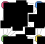
\includegraphics[width=.35\linewidth]{mc_state_transitions.pdf}
    \caption[Markov chain model of nucleotide substitutions]{
        \textbf{Markov chain model of nucleotide substitutions.}
        The evolution of characters at a site in an alignment can be modeled as a Markov chain (MC).
        The states of the MC for DNA data are the four nucleobases
        \nucleobase{A}, \nucleobase{C}, \nucleobase{G}, and \nucleobase{T}.
        The model allows transitions with rates $q_{ij}$ with $i,j \in \left\{~ A, C, G, T ~\right\}, i \neq j$ between all states,
        which correspond to substitutions of the nucleobases.
    }
    \label{fig:mc_state_transitions}
\end{figure}

% \begin{figure}[hpbt]
%  \begin{subfigure}[c]{.5\textwidth}
%     \centering
%     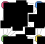
\includegraphics[width=.7\linewidth]{mc_state_transitions.pdf}
%     \caption{}
%     \label{fig:mc_state_transitions:sub:mc_chain}
%  \end{subfigure}
%  \begin{subfigure}[c]{.5\textwidth}
%     \begin{align*}
%         Q ~&=~
%          \begin{pmatrix}
%          ~-q_{A}   &   q_{AC}   &   q_{AG}   &   q_{AT}~~ \\
%          ~q_{CA}   &  -q_{C}    &   q_{CG}   &   q_{CT}~~ \\
%          ~q_{GA}   &   q_{GC}   &  -q_{G}    &   q_{GT}~~ \\
%          ~q_{TA}   &   q_{TC}   &   q_{TG}   &  -q_{T}~~
%          \end{pmatrix}
%         \\ \\
%         - q_{i} ~&=~ - \sum_{j \neq i} q_{ij}, ~ i = \left\{~ A, C, G, T ~\right\}
%     \end{align*}
%     \caption{}
%     \label{fig:mc_state_transitions:sub:matrix}
%   \end{subfigure}
%     \caption[Markov chain model of nucleotide substitutions]{
%         \textbf{Markov chain Model of Nucleotide Substitutions.}
%         The evolution of characters at a site in an alignment can be modeled as a Markov chain (MC).
%         \subref{fig:mc_state_transitions:sub:mc_chain} The states of the MC for DNA data are
%         the four nucleobases \nucleobase{A}, \nucleobase{C}, \nucleobase{G}, and \nucleobase{T}.
%         The model allows transitions between all states, which correspond to substitutions between the nucleobases.
%         \subref{fig:mc_state_transitions:sub:matrix} The instantaneous transition rates between states are given
%         by the substitution rate matrix (Q-matrix), where the rows must sum to $0$.
%     }
%     \label{fig:mc_state_transitions}
% \end{figure}

The process of state transitions is defined by the substitution rate matrix %$Q$

\begin{equation}
    \begin{align*}
        Q ~&=~
         \begin{pmatrix}
         ~-q_{A}   &   q_{AC}   &   q_{AG}   &   q_{AT}~~ \\
         ~q_{CA}   &  -q_{C}    &   q_{CG}   &   q_{CT}~~ \\
         ~q_{GA}   &   q_{GC}   &  -q_{G}    &   q_{GT}~~ \\
         ~q_{TA}   &   q_{TC}   &   q_{TG}   &  -q_{T}~~
         \end{pmatrix}
        \\ \\
        - q_{i} ~&=~ - \sum_{j \neq i} q_{ij}, ~ i \in \left\{~ A, C, G, T ~\right\}
    \end{align*}
\end{equation}

% The instantaneous transition rates between states are given
% by the substitution rate matrix (Q-matrix), where the rows must sum to $0$.
where the elements $q_{ij}$ are the \emph{instantaneous transition rates} from state $i$ to state $j$.
The rows of the $Q$-matrix have the requirement to sum to $0$,
by which the diagonal elements $q_{i}$ are defined.

The expected number of substitutions at an alignment site between two nodes of the tree
is expressed as the branch length $b$ between the nodes, and is a measure of evolutionary time $t$ between them.
Under the MC model, evolutionary time and branch length are proportional to each other
with the \emph{evolutionary rate} $r$ being their proportionality factor: $t = r \cdot b$.
Then, for a given time $t$, the \emph{transition probabilities} $p_{ij}(t)$ between states in a stationary process
are obtained by exponentiating the $Q$-matrix \cite{Yang2014}.
These probabilities are specified by the matrix

\begin{equation}
    \label{ch:Foundations:sec:MLTreeInference:eq:P_matrix}
    P(t) = e^{Qt}
\end{equation}

For positive transition rates $q_{ij} > 0, \forall i \neq j$, if the process runs long enough,
the Markov chain eventually reaches the unique \emph{stationary} distribution $\Pi = (\pi_A$, $\pi_C$, $\pi_G$, $\pi_T )$,
with $\pi_i$ being the proportion of time spent in state $i$.
If the Markov process reached equilibrium after running long enough,
it can be interpreted as having generated the sequences of the MSA.
In that case, $\Pi$ is the \emph{equilibrium base composition} of the MSA,
and $\pi_i$ are the \emph{equilibrium} or \emph{stationary base frequencies} of the MSA.

\paragraph{Time-Reversible Models}
\label{ch:Foundations:sec:MLTreeInference:sub:ModelsOfSeqEvol:par:TimeReversibleModels}

As mentioned before, most models of DNA evolution assume a \emph{time-reversible} Markov process,
which means that $\pi_{i} q_{ij} = \pi_{j} q_{ji} ~ \forall \, i \neq j$.
This assumption is biologically not meaningful, as evolution is a process in time, and thus does have a direction.
It however allows for simplified calculations:
The $Q$-matrix of a time-reversible model can be formulated as the product of
a symmetric rate matrix $R = \left\{ r_{i \leftrightarrow j} \right\}$ and
a diagonal matrix with the stationary base frequencies:

\begin{align}
    \newcommand{\lra}{\leftrightarrow}
    Q = R \cdot diag(\pi_i) =
    \begin{pmatrix}
         -q_A                       &   r_{A \lra C} \cdot \pi_C   &   r_{A \lra G} \cdot \pi_G   &   r_{A \lra T} \cdot \pi_T~~  \\
        ~r_{A \lra C} \cdot \pi_A   &   -q_C                       &   r_{C \lra G} \cdot \pi_G   &   r_{C \lra T} \cdot \pi_T~~  \\
        ~r_{A \lra G} \cdot \pi_A   &   r_{C \lra G} \cdot \pi_C   &   -q_G                       &   r_{G \lra T} \cdot \pi_T~~  \\
        ~r_{A \lra T} \cdot \pi_A   &   r_{C \lra T} \cdot \pi_C   &   r_{G \lra T} \cdot \pi_G   &   -q_T
    \end{pmatrix}
\end{align}

The matrix describes the most general model of DNA evolution,
where all \num{6} substitution rates $r_{i \leftrightarrow j}, i \neq j$ and
all \num{4} base frequencies $\pi_i$ can be different.
This model is called the Generalized Time-Reversible (\toolname{GTR}) model \cite{Tavare1986}.
As the sum of the base frequencies must be $1$,
and as the substitution rates are usually normalized by requiring that $r_{G \leftrightarrow T} = 1.0$,
the \toolname{GTR} model has a total of \num{8} free parameters
(that is, \num{3} base frequencies, and \num{5} substitution rates).
The base frequencies can also be estimated from the character frequencies in the given MSA,
in which case they are called the \emph{empirical} base frequencies.

There are also more restrictive models, which have fewer free parameters,
and are thus more robust if data for estimating them is sparse, at the expense of descriptiveness.
The Jukes-Cantor model (\toolname{JC69}) \cite{Jukes1969} has no free parameter
and assumes equal substitution rates $r_{i \leftrightarrow j} = 1$, $i \neq j$
and equal base frequencies $\pi_i = \sfrac{1}{4}$.
The \toolname{K80} model \cite{Kimura1980} adds a free parameter $\kappa$,
which describes the ratio between two types of substitutions that are not equally likely to occur in evolution:
$r_{A \leftrightarrow C} = r_{G \leftrightarrow T} = \kappa \cdot r_{A \leftrightarrow G} =
\kappa \cdot r_{A \leftrightarrow T} = \kappa \cdot r_{C \leftrightarrow G} = \kappa \cdot r_{C \leftrightarrow T}$.
% \todo{if transition vs transversion was added earlier, add it here, too!}
The \toolname{F81} model \cite{Felsenstein1981} instead extends the JC69
by allowing different base frequencies: $\pi_A \neq \pi_C \neq \pi_G \neq \pi_T$.
The \toolname{HKY85} model \cite{Hasegawa1985} combines the \toolname{K80} model and the \toolname{F81} model,
and hence has \num{4} free parameters.
Further models have also been proposed, which offer compromises
between the number of free parameters and the expressiveness of the model \cite{Yang2014}.

The state space of the Markov process becomes significantly larger for protein data,
as it needs to comprise \num{20} standard amino acids instead of \num{4} nucleobases.
Hence, the \toolname{GTR} model for protein data has $(400 - 20) / 2 - 1 + 19 = 208$ free parameters.
Typical amino acid alignments do not contain enough data to reliably estimate these parameters,
and thus easily lead to over-fitting.
Thus, so-called \emph{empirical} amino acid models are commonly used,
which have substitution rates and equilibrium base frequencies
that were pre-estimated on large collections of reference alignments.
Among others, some popular models include \toolname{DAYHOFF} \cite{Dayhoff1978},
\toolname{WAG} \cite{Whelan2001}, and \toolname{LG} \cite{Le2008}.

% ======================================================================================================================
%     Further Aspects of Tree Inference
% ======================================================================================================================

\subsection{Further Aspects of Tree Inference}
\label{ch:Foundations:sec:MLTreeInference:sub:FurtherAspects}

Evolution is an incredibly complex process with intricate details.
Many more models and methods have thus been proposed to refine tree inference \cite{Yang2014},
of which we here briefly introduce a few.
% For understanding the methods described in this work, the above introduction should suffice.
% For the distinguished reader, we here still mention a few other aspects that are related to the topic.
% While a detailed description of these models and methods is not necessary for understanding the main chapters of this work,
% we here still mention a few other related aspects.

\paragraph{Rate Heterogeneity}
\label{ch:Foundations:sec:MLTreeInference:sub:FurtherAspects:par:RateHeterogeneity}

The models of sequence evolution described above make the simplifying assumption
that the alignment sites evolve independently and are identically distributed.
However, certain regions of DNA or amino acid sequences are under higher evolutionary pressure than others,
for example if they describe important molecular functions that are conserved in their evolutionary history.
It is thus expected that some alignment sites evolve faster than others.
That is, the evolutionary rate $r$ of these sites is not constant across the alignment.
In the context of phylogenetic inference,
several models of \emph{rate heterogeneity among sites} have been proposed to account for this,
some of which are described in the following.

A simple model is the \emph{proportion of invariable sites},
where the likelihood of an alignment site is influenced by a parameter $p \in [0,1]$
that describes the proportion of sites that are assumed to be identical (\emph{invariable}) across all taxa.
The more elaborate $\Gamma$ model \cite{Yang1994a} postulates a shape parameter $\alpha > 0$
which models the rate heterogeneity as a gamma distribution $\Gamma(\alpha)$.
The distribution shape ranges from exponential-like ($\alpha < 1$, high rate heterogeneity)
to normal-like ($\alpha > 10$, low rate heterogeneity).
Thus, by optimizing the single free parameter $\alpha$,
different unimodal rate heterogeneity profiles can be approximated.
The \toolname{CAT} or \emph{per-site rates} model \cite{Stamatakis2006a}
is a compute- and memory-efficient approximation of the $\Gamma$ model,
which explicitly assigns one of $K$ rate categories to each alignment site instead of using a distribution of rates.
Lastly, the \toolname{FreeRate} model \cite{Yang1995} allows for multimodal distributions
by using $K$ rate categories and respective weights,
which can approximate any distribution at the cost of having to estimate these free parameters.

\paragraph{Alignment Partitioning}
\label{ch:Foundations:sec:MLTreeInference:sub:FurtherAspects:par:AlignmentPartitioning}

Apart from the evolutionary rate $r$, also the substitution patterns among the sites of an MSA can differ.
In order to account for this, the MSA can be split into different \emph{partitions},
where each such partition is assigned its own model of evolution.
For example, as three nucleobases code for one amino acid in regions that encode for proteins
(see \secref{ch:Foundations:sec:EvolutionGenetics}),
three partition can be used, each modeling the evolution of the first, second, and third nucleobase of each amino acid.
Furthermore, large multi-gene MSAs can be split into partitions corresponding to individual genes,
which might be under different evolutionary pressure each.

\paragraph{Constrained Trees}
\label{ch:Foundations:sec:MLTreeInference:sub:FurtherAspects:par:ConstrainedTrees}

The tree search (see \secref{ch:Foundations:sec:MLTreeInference:sub:TreeSearch})
can (theoretically) yield any topology from the vast space of possible trees.
It is however often serviceable to run a \emph{constrained} tree search,
for example to include prior knowledge about the taxa,
to maintain congruence with a given taxonomy, or because some other constraints are required.
Such a constraint can for example be specified by enforcing certain bipartitions to be retained in the tree,
that is, splits of the taxa that must be separated from each other in the tree.
As a bipartition is induced by a branch in the tree,
this is equivalent to starting the tree search with a multifurcating tree,
and then resolving these multifurcations without changing the other parts of the tree.
A constrained search yields a \emph{constrained tree}.

% Not needed:
% Alignment Partitioning

% ======================================================================================================================
%     Likelihood Computation
% ======================================================================================================================

\subsection{Likelihood Computation}
\label{ch:Foundations:sec:MLTreeInference:sub:LikelihoodComputation}

We here introduce the basic computational aspects of the Maximum Likelihood method.
For a more exhaustive description of the topic, see \cite{Yang2014}.
We assume a fixed tree topology $T$, fix branch lengths $\bar{b}$,
as well as a given model of sequence evolution $M$ with parameters $\bar{\theta}$.
That is, we do not cover the tree search itself here,
% \secref{ch:Foundations:sec:MLTreeInference:sub:TreeSearch}
but describe how to compute the likelihood $\mathcal{L}$
(\eqnref{ch:Foundations:sec:MLTreeInference:eq:likelihood}) for a given MSA under these conditions.

A central point of the ML method is to account for the unknown states at the inner nodes of the tree.
That is, the total likelihood is obtained by summing over the probabilities of every possible state of the inner nodes,
which can be efficiently computed by the \emph{Felsenstein pruning algorithm} (FPA) \cite{Felsenstein1981}.
It traverses the tree in post-order fashion, that is from the tips towards the (virtual) root,
and recursively calculates a so-called \emph{conditional likelihood vector} (CLV) at each inner node.

In a sense, a CLV summarizes the subtree below its corresponding node.
For every alignment site and every state,
it describes the \emph{conditional likelihood} of the node to be in that state at that site,
given the subtree topology and its branch lengths, for the respective subset of the alignment (tip sequences).
We here assume a set $N$ of states, that is, the sequences consist of characters $c \in N$,
for example $N = \left\{~ \nucleobase{A}, \nucleobase{C}, \nucleobase{G}, \nucleobase{T} ~\right\}$.
Furthermore, for simplicity, we do not consider alignment partitioning or rate heterogeneity among sites here,
and thus use a fixed evolutionary rate $r$.
Then, a CLV contains $|N|$ elements per alignment site,
each describing the conditional likelihood of being in the corresponding state.
For DNA data, these are CL(\nucleobase{A}), CL(\nucleobase{C}), CL(\nucleobase{G}), and CL(\nucleobase{T}).

\paragraph{Felsenstein Pruning Algorithm}
\label{ch:Foundations:sec:MLTreeInference:sub:LikelihoodComputations:par:FPA}

In order to start the recursion of the FPA, first, the CLVs at the tip nodes have to be initialized.
In principle, these can be the actual likelihoods of observing the characters $c \in N$ at the corresponding site.
However, this uncertainty is rarely available in empirical data.
Thus, tip nodes are usually initialized with ``pseudo-CLVs'',
where for instance a nucleobase \nucleobase{A} in the alignment yields
CL(\nucleobase{A}) $= 1$, and CL(\nucleobase{C}) $=$ CL(\nucleobase{G}) $=$ CL(\nucleobase{T}) $= 0$.

\begin{figure}[pthb]
    \centering
    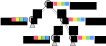
\includegraphics[width=.85\linewidth]{clv_fpa.pdf}
    \caption[Felsenstein pruning algorithm]{
        \textbf{Felsenstein pruning algorithm.}
        An exemplary tree topology with a (virtual) root {\sffamily R}, an inner node {\sffamily V},
        and three other nodes {\sffamily U}, {\sffamily L}, and {\sffamily M},
%         (which can be either tips or inner nodes),
        and branch lengths between nodes.
        Potential subtrees are marked by triangles below nodes.
%         For the recursive computation during Felsenstein's pruning,
%         Because of the recursive nature of the algorithm,
%         it is irrelevant whether the last three nodes are tips or have subtrees (marked here by triangles below them).
        \\
        Each node has a CLV assigned to it, which ``summarizes'' the subtree below it.
        A CLV stores a conditional likelihood for every alignment site and for every state.
        Here, for simplicity, we show the CLVs for one site and for four states,
        which for instance represent the likelihood of that site to be in either state of the four nucleobases.
        %\nucleobase{A}, \nucleobase{C}, \nucleobase{G}, and \nucleobase{T}.
%         Lastly, the branches of the tree have branch lengths assigned to them.
    }
    \label{fig:clv_fpa}
\end{figure}

After the tip CLVs have been initialized, the algorithm traverses up the tree, see \figref{fig:clv_fpa}.
This can be thought of as moving along the branches towards a parent node,
which induces the possibility of state transitions.
This step is thus where the model $M$ is employed (see \secref{ch:Foundations:sec:MLTreeInference:sub:ModelsOfSeqEvol}).
As we assumed a fixed evolutionary rate $r$,
we can infer the time $t$ between two nodes from the branch length $b$ between them: $t = r \cdot b$.
% Then, in order to compute the likelihood of state changes while moving from a child node to its parent,
% the model $M$ is employed, as explained in \secref{ch:Foundations:sec:MLTreeInference:sub:ModelsOfSeqEvol}.
% In particular,
Then, for a given branch, we can compute the probability $p_{ij}(t)$ of a transition
from state $i$ to state $j$ after moving along the branch, see \eqnref{ch:Foundations:sec:MLTreeInference:eq:P_matrix}.
Note that the probability $p_{ij}$ depends on the branch length,
meaning that for every branch (and every update in its branch length during optimization,
see \secref{ch:Foundations:sec:MLTreeInference:sub:BLO}),
a separate $P$-matrix has to be computed from the $Q$-matrix of the model.

At a parent node whose children have been computed, we can now apply the recursion step of the algorithm.
For instance, in the topology shown in \figref{fig:clv_fpa}, the CLV of an inner node {\sffamily V}
can be computed given its children {\sffamily L} and {\sffamily M}.
For the computation, the CLVs of the two child nodes,
as well as the transition probabilities $p_{ij}$ for the branch lengths $b_{LV}$ and $b_{MV}$
of the branches towards the parent are needed.
% and the respective branch lengths $b_{LV}$ and $b_{MV}$.
Then, a single entry of the CLV, that is,
the conditional likelihood of node {\sffamily V} to be in state $c$ at site $s$, is

\begin{equation}
    \label{ch:Foundations:sec:MLTreeInference:eq:CLV}
%     \mbox{CLV} =
    \mbox{CLV}^{(V)}_{s,c} =
    \left(~ \sum_{j \in N} p_{cj}(r \cdot b_{LV}) \cdot \mbox{CLV}^{(L)}_{s,j} \right)
    \left(~ \sum_{k \in N} p_{ck}(r \cdot b_{MV}) \cdot \mbox{CLV}^{(M)}_{s,k} \right)
\end{equation}

The equation can be interpreted as follows:
The product of transition probability and conditional likelihood represents a change from state $c$ to another state in $N$.
By summing this product for all states, all possible inner states are accounted for.
Finally, the product of the two sums is the new conditional likelihood of the node being in state $c$ at site $s$,
given the evolutionary history of its children and their subtrees.

By repeating the computation for every state $c \in N$ and every site $s$ of the alignment,
the complete CLV for node {\sffamily V} is computed.
The recursion is then applied to all nodes upwards the tree, until all CLVs are computed.

\paragraph{Likelihood Evaluation at the Root}
\label{ch:Foundations:sec:MLTreeInference:sub:LikelihoodComputations:par:RootLikelihood}

Once all CLVs are computed, the overall likelihood $\mathcal{L}$ can be computed from the CLV of the root node.
Given the root node {\sffamily R} as shown in \figref{fig:clv_fpa},
the total \emph{per-site likelihood} $\mathcal{L}_s$ of an alignment site $s$ is
accumulated from the conditional likelihoods of all states,
taking their respective base frequencies $\pi_i$ into account:

\begin{equation}
    \label{ch:Foundations:sec:MLTreeInference:eq:root_site_likelihood}
    \mathcal{L}_{s} = \sum_{i \in N} \pi_i \cdot \mbox{CLV}^{(R)}_{s,i}
\end{equation}

Due to the time reversibility of the model, for unrooted trees, a \emph{virtual} root can be used,
that is, an additional node that is presumed to be present on a branch of the tree.
% The calculation is invariant to the exact position of this node along the branch.
% which might coincide with an actual node of the tree
If for example the node {\sffamily R} in \figref{fig:clv_fpa} represents a virtual root,
the two branches between nodes {\sffamily U} and {\sffamily V}
are actually one branch with branch length $b_{UV} = b_{UR} + b_{VR}$.
Then, an alternative way of computing the per-site likelihood is what we here call the (per-site) \emph{edge likelihood}.
Instead of using the CLV at the virtual root {\sffamily R}, we can use the CLVs of {\sffamily U} and {\sffamily V},
and the corresponding branch length $b_{UV}$ for the computation.
In that case, state transitions along the branch have to be additionally accounted for in the computation.
The per-site edge likelihood of an alignment site $s$ can then be computed as

\begin{equation}
    \label{ch:Foundations:sec:MLTreeInference:eq:edge_likelihood}
    \mathcal{L}_{s} = \sum_{i \in N} \sum_{j \in N} \pi_i \cdot \mbox{CLV}^{(U)}_{s,i} \cdot
    p_{ij}(r \cdot b_{UV}) \cdot \mbox{CLV}^{(V)}_{s,j}
\end{equation}

This way of calculating the edge likelihood $\mathcal{L}_s$ works for any two adjacent nodes,
if their respective CLVs have been computed to represent the two subtrees induced by the branch between the nodes.

Finally, the overall likelihood $\mathcal{L}( \mbox{MSA} ~|~ T, \bar{b}, M, \bar{\theta} )$
for the entire MSA can be computed.
For mathematical simplicity, the sites are generally assumed to evolve independently,
although this is not expected to be the case from a biological perspective.
Then, for an alignment with $m$ sites, the overall likelihood is simply the product of the per-site or edge likelihoods:

\begin{equation}
    \label{ch:Foundations:sec:MLTreeInference:eq:root_likelihood}
    \mathcal{L} = \prod_{s=1}^{m} \mathcal{L}_s
\end{equation}

For computational reasons, and to avoid numerical underflow, in practice,
the logarithm of the likelihood (\emph{log-likelihood}) is typically used.
Furthermore, as identical sites yield exactly the same likelihood,
such sites are often compressed and the respective likelihood is multiplied with an according \emph{weight}.
% Lastly, we note that the derivatives of the above likelihood functions can be obtained analytically \cite{Yang2014},
% which is needed for optimizing the branch lengths,
% as explained in \secref{ch:Foundations:sec:MLTreeInference:sub:TreeSearch}.

% ======================================================================================================================
%     Branch Length Optimization
% ======================================================================================================================

\subsection{Branch Length Optimization}
\label{ch:Foundations:sec:MLTreeInference:sub:BLO}

Another important aspect of the tree search
is the optimization of the branch lengths of the tree.
That is, for a given tree topology $T$, and a fixed model $M$ with parameters $\bar{\theta}$,
we want to compute the branch lengths $\bar{b}$
that maximize the likelihood $\mathcal{L}( \mbox{MSA} ~|~ T, \bar{b}, M, \bar{\theta} )$.
This procedure is called \emph{branch length optimization} (BLO),
and typically uses the Newton-Raphson method \cite{Ypma1995},
as mentioned in \secref{ch:Foundations:sec:MLTreeInference:sub:TreeSearch}.

We consider to optimize a single branch length $b$.
In order to maximize $\mathcal{L}$, we need to find the root of the first derivative $\mathcal{L}'$.
The Newton-Raphson method takes an initial value for $b$ and then
iteratively approximates values that lead closer to the root:

\begin{equation}
    \label{ch:Foundations:sec:MLTreeInference:eq:BLO}
    b_{n+1} = b_n - \frac{ \mathcal{L}' }{ \mathcal{L}'' }
\end{equation}

Note that the derivatives $\mathcal{L}'$ and $\mathcal{L}''$ can be obtained analytically \cite{Yang2014},
and have to be computed in every iteration.
The algorithm stops when the change in $b$ between two iterations is below a threshold,
that is, when then optimization \emph{converges}.
This procedure is repeated for all branch lengths $\bar{b}$ in the tree.

% ######################################################################################################################
%         Phylogenetic Placement
% ######################################################################################################################

\section{Phylogenetic Placement}
\label{ch:Foundations:sec:PhylogeneticPlacement}

In studies of sequence data, one of the most common tasks is a phylogenetic analysis of the data,
that is, to infer the evolutionary context of the sequences.
However, since the amount of sequence data produced in typical metagenomic studies can be quite substantial,
computational challenges and bottlenecks arise \cite{Scholz2012}.
In particular, both calculating an MSA and inferring a phylogeny are NP-hard \cite{Just2001,Chor2005},
and thus impractical or infeasible for large datasets.
Furthermore, metagenomic reads are often short, and hence lack phylogenetic signal
to robustly infer a tree and to properly resolve their relationships.

Thus, \emph{phylogenetic placement}, also called \emph{evolutionary placement},
has been developed for conducting phylogenetic analyses of such data,
as implemented in tools such as
\toolname{pplacer} \cite{Matsen2010}, \toolname{RAxML-EPA} \cite{Berger2011}, and \toolname{EPA-ng} \cite{Barbera2018}.
% cited more than 630 times (as of 2018-07-01)
Instead of resolving the phylogeny of a set of metagenomic sequences,
phylogenetic placement treats each sequence, called a \emph{\acl{QS}}\acused{QS} (\acs{QS}), separately.
It evaluates how these \acp{QS} relate to an existing \emph{\acl{RT}}\acused{RT} (\acs{RT}) based on known reference sequences.
For each \ac{QS}, it computes the probabilities of \emph{placing} the sequence on the branches of the \ac{RT},
% In other words, it maps the \acp{QS} of interest onto the branches of an \ac{RT},
thereby classifying them into a phylogenetic context of related sequences,
without the need to resolve relationships between the \acp{QS}.

Phylogenetic placement can be carried out if the \acp{QS} can be aligned to the alignment of the reference sequences.
In the most common use case, the \acp{QS} are reads or amplicons from environmental samples.
Most often barcoding regions or marker genes such as 16S or 18S are used
(see \secref{ch:Foundations:sec:SequenceAnalysis:sub:Metagenomics}),
but there also exist studies that use different, or even a set of, maker genes \citep{Sunagawa2013a}.
Furthermore, other types of sequences such as \textsubscript{mi}tags \citep{Logares2014} can be used.

The \ac{RT} and the reference sequences it represents are typically assembled by the user
so that they capture the expected species diversity in the samples.
We however proposed an automated approach for assembling suitable sets of reference sequences \cite{Czech2018},
which we describe in \chpref{ch:AutomaticTrees}.
Distinct samples from one study are typically placed on the same underlying \ac{RT}
in order to facilitate comparisons between the samples,
see \secref{ch:Foundations:sec:PhylogeneticPlacement:sub:ExistingMethods}.
% Such a mapping also elucidates the evolutionary distance between the query and the reference sequences,
% see \secref{ch:Foundations:sec:PhylogeneticPlacementAnalysis:sub:Distances}.

% The result of phylogenetic placement is a mapping of the query sequences to the branches of the reference tree.
% In brief, phylogenetic placement calculates the most probable insertion branches for each given \acf{QS} on a \acf{RT}.

% In short, for a given \acf{QS}, phylogenetic placement computes a mapping of the \ac{QS}
% to the most closely related branches of a fixed \acf{RT} based on known reference sequences.
% Phylogenetic placement uses a fixed \acf{RT} based on known reference sequences to compute a mapping
% of \acfp{QS} to the branches of the tree that are most closely related to the \ac{QS}.
% This mapping classifies the \acp{QS} (e.g., sequences from a metagenomic study) into a phylogenetic context

% ======================================================================================================================
%     Pipeline and Computation
% ======================================================================================================================

\subsection{Pipeline and Computation}
\label{ch:Foundations:sec:PhylogeneticPlacement:sub:PipelineAndComputation}

% \todo{pipeline diagram, data flow, etc, reference to chapters?!}

% \paragraph{Preparation}
% \label{ch:Foundations:sec:PhylogeneticPlacement:sub::par:Preparation}

We here assume to have given a set of suitable reference sequences, their alignment, and an \ac{RT} inferred from them.
As phylogenetic placement used a maximum likelihood criterion, the \ac{RT} has to be strictly bifurcating.
Prior to the placement, the \acp{QS} need to be aligned against the reference alignment of the \ac{RT}
by programs such as \toolname{PaPaRa} \cite{Berger2011a,Berger2012} or \toolname{hmmalign} \cite{Eddy1998,Eddy2009},
see also \secref{ch:Foundations:sec:SequenceAnalysis:sub:SequenceAlignment}.
The input to phylogenetic placement are then the \acf{RT}, its underlying alignment, and the aligned \acfp{QS}.

\paragraph{Computation for one Query Sequence}
\label{ch:Foundations:sec:PhylogeneticPlacement:sub:PipelineAndComputation:par:ComputingQuerySequence}

% The placement is then conducted for each \ac{QS} separately
% by initially inserting a \ac{QS} as a new tip into a branch of the tree,
% then re-optimizing the branch lengths that are most affected by the insertion,
% and thereafter evaluating the resulting likelihood score of the tree.
% The \ac{QS} is then removed from the current branch and subsequently placed into all other branches of the \ac{RT}.

The placement is conducted for each \ac{QS} separately, always using the same fixed \ac{RT} as a starting point.
Each branch of the tree is evaluated as a potential \emph{placement location} of the \ac{QS},
which indicates how likely the branch is to be the ancestor of the \ac{QS}.
In \figref{fig:tiny_tree},
the procedure for one \ac{QS} and one branch (between nodes {\sffamily D} and {\sffamily P}) is shown:
The sequence is inserted as a new tip node {\sffamily Q} on the branch,
connected to it by a new \emph{pendant} branch and a new node {\sffamily C}.
This splits the original branch into two parts, called the \emph{distal} and the \emph{proximal} branch, respectively,
which are named according to the direction of the root of the tree.
Note that the tree can also be unrooted, in which case a top-level trifurcation is typically used as root.

\begin{figure}[pthb]
    \centering
    
\includegraphics[width=.7\linewidth]{tiny_tree.pdf}
    \caption[Terminology of a phylogenetic placement]{
        \textbf{Terminology of a phylogenetic placement.}
        The nodes {\sffamily D} and {\sffamily P} belong to the reference tree (RT).
        When placing a query sequence (QS), the branch between them %{\sffamily D} and {\sffamily P}
        is split into two parts by a new node {\sffamily C},
        which serves as the attachment point for another new node {\sffamily Q} that represents the QS.
        The \emph{pendant} branch leads to {\sffamily Q}.
        The original branch is split into the \emph{proximal} branch, which leads towards the root of the RT,
        and the \emph{distal} branch, which leads away from the root.
    }
    \label{fig:tiny_tree}
\end{figure}

In the next step, the branch lengths of the tree are optimized,
as explained in \secref{ch:Foundations:sec:MLTreeInference:sub:BLO}.
After the optimization, the sum of the lengths of the distal and proximal branches is not necessarily equal
to the original branch length between {\sffamily D} and {\sffamily P}.
Thus, typically, the two lengths are proportionally rescaled to maintain this equality.

Lastly, the likelihood of the tree with the newly attached sequence is evaluated
as explained in \secref{ch:Foundations:sec:MLTreeInference:sub:LikelihoodComputation}.
Note that the likelihood computation uses the MSA (extended by the query sequence),
the tree topology and branch lengths, as well as the model and its parameters as before.
The model of nucleotide evolution should be the same that was used when inferring the tree,
see \secref{ch:Foundations:sec:MLTreeInference:sub:ModelsOfSeqEvol}.
% mention that epa ng can use all the model stuff explaine above: subst models, rate hetero, etc
After this, the newly created nodes on the branch are removed again, thus restoring the original reference tree.

The above procedure is repeated for every branch $i$ of the tree $T$,
yielding a set of likelihood scores $\mathcal{L}(i)$ for each possible placement location.
Thus, for each branch of the tree, the process yields a so-called \emph{placement} of the \ac{QS},
that is, an optimized position on the branch, along with a likelihood score for the whole tree.
The likelihood scores for a \ac{QS} are then transformed into probabilities,
which quantify the uncertainty of placing the sequence on the respective branch \cite{Strimmer2002,VonMering2007}.
The probability of placing a \ac{QS} on a branch $q$ is called the \emph{\acl{LWR}}\acused{LWR} (\acs{LWR}),
and is calculated relative to the other branches $i$ of the tree $T$ as

\begin{equation}
    \label{ch:Foundations:sec:PhylogeneticPlacement:eq:LWR}
    \mbox{LWR}(q) =  \frac{ \mathcal{L}( q )}{ \sum_{i \in T} \mathcal{L}( i )}
\end{equation}

By construction, the sum of the \acp{LWR} of all branches for a single \ac{QS} is $1.0$.
It can thus be interpreted as a probability distribution over the branches of the tree,
as shown in \figref{fig:tree_epa}.
For most use cases, the \acp{LWR} and the respective placement on the branches are the most important values,
while pendant lengths are rarely used in downstream analyses.
However, long pendant lengths can indicate that the \ac{RT} is missing sequences that are closely related to the \ac{QS}.

\begin{figure}[hpbt]
    \centering
    \includegraphics[width=.6\linewidth]{pppp/tree_epa.pdf}
    \caption[Phylogenetic Placement of a Query Sequence]{
        \textbf{Phylogenetic Placement of a Query Sequence.}
        Each branch of the reference tree is tested as a potential insertion position, called a \emph{placement}
        (blue dots; pendant lengths are ignored here).
        Note that placements have a specific position on their branch, due to the branch length optimization process.
        A probability of how likely it is that the sequence belongs to a specific branch is computed
        (numbers next to dots),
        which is called the \emph{likelihood weight ratio} (LWR).
%         based on the maximum likelihood score of the whole tree. %(that is, including the query sequence)
        The bold number (0.7) denotes the most probable placement of the sequence.
    }
    \label{fig:tree_epa}
\end{figure}

\paragraph{Accelerations}
\label{ch:Foundations:sec:PhylogeneticPlacement:sub:PipelineAndComputation:par:Accelerations}

The most expensive part of the placement computation are the branch lengths optimizations.
Thus, several techniques have been developed to accelerate the placement process \cite{Barbera2018}.

Firstly, above, all branches of the tree were optimized when evaluation a placement location,
which gives the most accurate results.
In practice however, it suffices to only optimize the three branches of the placement location
without losing too much accuracy.

Secondly, because the reference tree is fixed (except for the newly created nodes),
the CLVs of all possible subtrees can be precomputed,
which drastically accelerates the likelihood evaluation.
Using \figref{fig:tiny_tree} as an example,
with two CLVs of the nodes {\sffamily D} and {\sffamily P}, and one application of the Felsenstein Pruning Algorithm
(see \secref{ch:Foundations:sec:MLTreeInference:sub:LikelihoodComputations:par:FPA}),
the CLV of node {\sffamily C} can be computed.
Then, the final likelihood can be evaluated as the edge likelihood of the pendant edge,
using this CLV as well as the pseudo-CLV of node {\sffamily Q}.

Thirdly, further acceleration can be achieved with a \emph{pre-placement} heuristic:
A first approximate evaluation of a placement location can be conducted by using
distal and proximal lengths based on the respective original branch length of the tree, and a fixed default pendant length.
Then, only the most likely fraction of locations is thoroughly evaluated, that is, including branch length optimizations.
This way, millions or even billions of sequences can be placed within acceptable time \cite{Barbera2018}.
This is however a heuristic that might lead to suboptimal results by ignoring placement locations
whose \ac{LWR} is significantly improved by the branch length optimization process.
If the \ac{RT} is however well suited for the \acp{QS}, this situation is generally not expected to occur.

\paragraph{Placement Result}
\label{ch:Foundations:sec:PhylogeneticPlacement:sub:PipelineAndComputation:par:PlacementResults}

The placement process is repeated independently for every \ac{QS}.
That is, for each \ac{QS}, the algorithm starts calculating placements from scratch on the original \ac{RT}.
The result thus classifies each \ac{QS} in the phylogenetic context of the \ac{RT},
without resolving the evolutionary relationships between the \acp{QS}.

The data is usually stored in so-called \fileformat{jplace} files \cite{Matsen2012},
which is a standard based on the \fileformat{JSON} format \cite{JsonMemo,JsonStandard}.
It stores the \ac{RT} in \fileformat{Newick} format, including tip names and branch lengths,
and extended by a post-order numbering of the edges to be referenced by the placements.
The main part of the file is a list of lists:
For each \ac{QS}, its list of placements is stored.
A placement is described by its edge number (referencing the \ac{RT}),
the \ac{LWR}, the pendant length, and the distal length.
The proximal length is usually omitted, as it can be inferred from the branch length of the tree.
Furthermore, the format can summarize multiple identical \acp{QS}
by allowing several names for each list of placements,
where each name can also have a weight (called its \emph{multiplicity}).
Lastly, usually not all placement locations are stored in the file,
as the ones with low \ac{LWR} do not contribute much to post-analysis methods anyway.

% In summary, the result of a phylogenetic placement analysis is a mapping of the \acp{QS} in a sample
% to positions on the branches of the \ac{RT}.
% Each such position, along with the corresponding \ac{LWR}, is called a placement of the \ac{QS}.
% The result of phylogenetic placement is a mapping of each \ac{QS} (e.g., environmental reads)
% to positions on the branches of the \ac{RT}, amended by probabilities in form of their likelihood weight ratios.
% Each \ac{QS} is thus represented by its placement positions, which are also called its placements.
% along with the respective likelihood weight ratios.f

% Each such sample represents a geographical location, a body site, a point in time, etc.
% In the following, we represent a sample by the placement locations of its metagenomic \acp{QS},
% including the respective per-branch \acp{LWR}.
% Furthermore, for a specific analysis, we assume the standard use case,
% that is, all placements were computed on the same fixed \acf{RT} and \acl{RA}.

% ======================================================================================================================
%     Use Cases and Applications
% ======================================================================================================================

\subsection{Use Cases and Applications}
\label{ch:Foundations:sec:PhylogeneticPlacement:sub:UseCasesApplications}

Phylogenetic placement is a flexible tool that yields useful biological information \emph{per se},
but that also can be utilized for a variety of downstream analyses.

\paragraph{Comparison to Existing Methods}
\label{ch:Foundations:sec:PhylogeneticPlacement:sub:UseCasesApplications:par:Comparison}

A typical task in metagenomic studies is to identify and classify the environmental sequences with respect
to known reference sequences, either in a taxonomic or phylogenetic context,
as mentioned in \secref{ch:Foundations:sec:SequenceAnalysis:sub:Metagenomics}.
Conventional methods for this task, such as \toolname{BLAST} \cite{Altschul1990}, are based on sequence similarity.
Such methods are fast, but only attain satisfying accuracy levels
if the query sequences are sufficiently similar to the reference sequences.
Furthermore, the best \toolname{BLAST} hit does often \emph{not} represent the most closely related species \cite{Koski2001}.
This is particularly true for environments where available reference databases do not exhibit
sufficient taxon coverage \citep{Mahe2017}.
Moreover, as insufficient taxon coverage cannot be detected by methods that are based on sequence similarity,
they can potentially bias downstream analyses.

More recent methods can alleviate some of these issues, for instance by
using machine learning techniques to obtain a taxonomic classification of metagenomic sequences \cite{Vervier2015},
or by utilizing a phylogeny inferred from metagenomic OTUs to classify microbial communities \cite{Tanaseichuk2014}.
However, the common shortcoming of these methods is
that they lack a way of incorporating phylogenetic information of known sequences.

A phylogenetic placement analysis \emph{does} incorporate known phylogenetic relationships,
and hence provides a more accurate means for read identification and classification.
For example, the classification of query sequences
can be summarized by means of sequence abundances \cite{Pace1997,Hugenholtz1998},
or to obtain taxonomic assignments \cite{Kozlov2016}.

However, phylogenetic placement also allows for more elaborate downstream analyses.
Firstly, the reference tree usually offers a higher resolution than simple per-taxon abundance counts,
and the amount of mapped \acp{QS} per branch can be directly visualized on the \ac{RT} \citep{Mahe2017},
as shown in \secref{ch:Visualization:sec:Motivation}.
Secondly, established methods such as Edge PCA and Squash Clustering \citep{Matsen2011a},
which we introduce in \secref{ch:Foundations:sec:PhylogeneticPlacement:sub:ExistingMethods},
allow for identifying subtle differences between distinct samples,
thus enabling comparative studies directly based on phylogenetic placement.
Lastly, we proposed novel methods for visualizing and clustering phylogenetic placement data \citep{Czech2018a},
which we describe in \chpref{ch:Visualization} and \chpref{ch:Clustering}.
Another typical task in metagenomic studies is to discover novel diversity within the samples,
which can be conducted using phylogenetic placement, as outlined in \chpref{ch:ConclusionOutlook}.

\paragraph{Variants and Derived Tools}
\label{ch:Foundations:sec:PhylogeneticPlacement:sub:UseCasesApplications:par:DerivedTools}

There also exist variants of phylogenetic placement that use maximum parsimony \cite{Berger2011}
and minimum evolution \cite{Filipski2015} instead of maximum likelihood,
and variants that calculate Bayesian posterior probabilities \cite{Matsen2010}.
The boosting method \toolname{SEPP} has been proposed to improve the accuracy of the placements \cite{Mirarab2012}.
The recently proposed tool \toolname{RAPPAS} \cite{Linard2018} is an alignment-free approach
that is not based on ML, but yields comparable results to standard phylogenetic placement implementations.

Phylogenetic placement has further been used for a variety of applications and derived pipelines, such as
species delimitation as in \toolname{PTP} \cite{Zhang2013} and \toolname{mPTP} \cite{Kapli2017},
genome and metagenome analysis as in \toolname{PhyloSift} \cite{Darling2014},
taxonomic identification and phylogenetic profiling as in \toolname{TIPP} \cite{Nguyen2014}, and
identification and correction of taxonomically mislabeled sequences as in \toolname{Sativa} \cite{Kozlov2016}.

% these tools combine 1,010 more citations (as of 2018-07-01)

% ======================================================================================================================
%     Placement Processing
% ======================================================================================================================

\subsection{Placement Processing}
\label{ch:Foundations:sec:PhylogeneticPlacement:sub:PlacementProcessing}

% \paragraph{Normalization}
% \label{ch:Foundations:sec:PhylogeneticPlacement:sub:PlacementProcessing:par:Normalization}

When placing multiple environmental samples, for instance, from different geographical locations,
typically, the same \ac{RT} is used, in order to allow for comparisons of the phylogenetic composition of these samples.
In this context, it is important to consider how to properly normalize the samples.
Normalization is required as the sample size (often also called library size),
that is, the number of sequences per sample, can vary by several orders of magnitude,
due to efficiency variations in the sequencing process or biases introduced by the amplification process,
as explained in \secref{ch:Foundations:sec:SequenceAnalysis:sub:Metagenomics}.

Selecting an appropriate normalization strategy hence constitutes a common problem in many metagenomic studies.
The appropriateness depends on data characteristics \cite{Weiss2017}, but also on the biological question asked.
For example, estimating indices such as the species richness are often implemented
via so-called \emph{rarefaction} and rarefaction curves \cite{Gotelli2001}
by randomly re-drawing sequences from the set of sequences in a sample to obtain comparable sample sizes.
This however ignores a potentially large amount of the available valid data \cite{McMurdie2014}.
Furthermore, the specific type of input sequence data has to be taken into account for normalization:
Biases induced by the amplification process can potentially be avoided if, instead of amplicons,
data based on shotgun sequencing are used, such as \textsubscript{mi}tags \cite{Logares2014}.
Moreover, similar sequences can be clustered prior to phylogenetic placement analysis, for instance,
by constructing so-called \emph{operational taxonomic units} (OTUs) \cite{Edgar2010,Mahe2014,Mahe2015,Rognes2016}.
Analyses using OTUs focus on species diversity instead of simple abundances.
OTU clustering substantially reduces the number of sequences,
and hence greatly decreases the computational cost for placement analyses.
Lastly, one may completely ignore the abundances (which correspond to the \emph{multiplicities} of placements)
of the placed sequences, reads, or OTUs, and only be interested in their presence/absence when comparing samples.

Which of the above analysis strategies is deployed,
depends on the specific design of the study and the research question at hand.
The common challenge is that the number of sequences per sample differs, which affects most post-analysis methods.

In the following, we therefore explain how the necessary normalizations of sample sizes can be performed.
We also introduce established terminology,
and describe general techniques for interpreting and working with phylogenetic placement data.
These are not methods of their own, but they are tools and building blocks
that are necessary for the analysis methods explained and introduced later.

\paragraph{Edge Masses}
\label{ch:Foundations:sec:PhylogeneticPlacement:sub:PlacementProcessing:par:EdgeMasses}

Methods that compare samples directly based on their sequences,
such as the UniFrac distance \cite{Lozupone2005,Lozupone2007a},
can benefit from rarefaction \cite{Weiss2017}.
However, in the context of phylogenetic placement, rarefaction is not necessary.
Thus, more valid data can be kept.
To this end, it is convenient to think of the reference tree as a graph.
% (when exploiting graph properties of the tree, we refer to the branches of the tree as edges).
Then, the per-branch \acp{LWR} for a single \ac{QS}
can be interpreted as mass points distributed over the edges of the \ac{RT},
including their respective placement positions on the branches, as shown in \figref{fig:tree_epa}.
We call this the \emph{mass interpretation} of the placed \acp{QS},
and henceforth use mass and \ac{LWR} interchangeably.
For simplicity, we here ignore that typically not all placements are stored in \fileformat{jplace} files,
meaning that the mass per QS can also be $<1$.
Hence, each \ac{QS} is assumed to have a total accumulated mass of $1.0$ on the \ac{RT}.
The \emph{mass of an edge} or \emph{edge mass} refers to the sum of the \acp{LWR} on that edge for all \acp{QS} of a sample,
as shown in \figref{fig:imbalance:sub:ReferenceTree}.
The \emph{total mass} of a sample is then the sum over all edge masses,
which is identical to the number of \acp{QS} in the sample,

\begin{figure}[!ht]
    \centering
    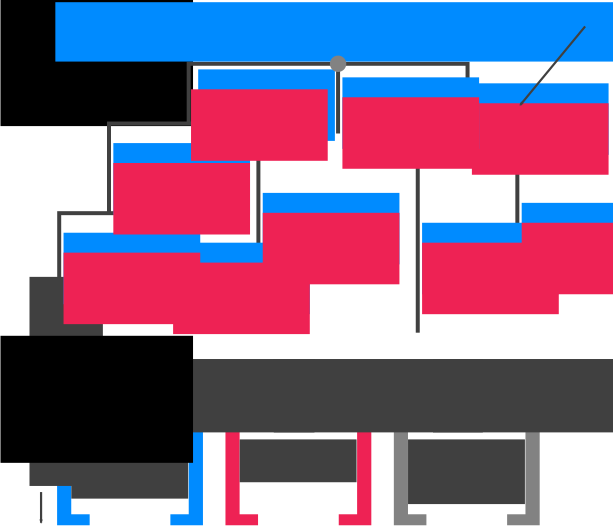
\includegraphics[width=0.8\linewidth]{imbalance.pdf}
    \begin{subfigure}{0pt}
        \phantomcaption
        \label{fig:imbalance:sub:ReferenceTree}
    \end{subfigure}
    \begin{subfigure}{0pt}
        \phantomcaption
        \label{fig:imbalance:sub:Matrices}
    \end{subfigure}
    \caption[Edge Masses and Imbalances]{
        \textbf{Edge Masses and Imbalances.}
        \subref{fig:imbalance:sub:ReferenceTree}
        Reference tree where each edge is annotated with the normalized mass (first value, blue) and
        imbalance (second value, red) of the placements in a sample.
        The imbalance is the sum of masses on the root side of the edge minus the sum of the masses on the non-root side.
        The depicted tree is unrooted, hence, its top-level trifurcation (gray dot) is used as ``root'' node.
        An exemplary calculation of the imbalance is given at the top.
        Because terminal edges only have a root side, their imbalance is not informative.
        \subref{fig:imbalance:sub:Matrices}
        The masses and imbalances for the edges of a sample constitute the rows of the first two matrices.
        The third matrix contains the available meta-data features for each sample.
        These matrices are used to calculate, for instance, the edge principal components or correlation coefficients.
    }
    \label{fig:imbalance}
\end{figure}

The key idea is to use the distribution of placement mass points over the edges of the \ac{RT} to characterize a sample.
This allows for normalizing samples of different size
by scaling the total sample mass to unit mass $1.0$.
In other words, absolute abundances are converted into relative abundances.
This way, rare species, which might have been removed by rarefaction, can be kept,
as they only contribute a negligible mass to the branches into which they have been placed.
This approach is analogous to using proportional values for methods based on OTU count tables,
that is, scaling each sample/column of the table by its sum of OTU counts \cite{Weiss2017}.
Most of the methods presented here use normalized samples, that is, they use relative abundances.
As relative abundances are compositional data, certain caveats occur \cite{Aitchison1986,Lovell2015,Gloor2016},
which we discuss where appropriate.

When working with large numbers of \acp{QS},
the mass interpretation allows to further simplify and reduce the data:
The masses on each edge of the tree can be quantized into $b$ discrete bins,
that is, each edge is divided into $b$ intervals (or bins) of the corresponding branch length.
All mass points on that edge are then accumulated into their respective nearest bin.
For example, by accumulating mass points at their nearest interval midpoint, masses are only minimally moved.
The parameter $b$ controls the resolution and accuracy of this approximation.
In the extreme case of $b:=1$, all masses on an edge are grouped into one single bin.
This \emph{branch binning} process drastically reduces the number of mass points
that need to be stored and analyzed in several methods we present,
while only inducing a negligible decrease in accuracy.
As shown in \tabref{tab:hmp_binning_error}.
branch binning can yield a speedup of up to 75\% for post-analysis run-times.

Furthermore, using masses allows to summarize a set of samples
by annotating the \ac{RT} with their average per-edge mass distribution.
This procedure, also called \emph{squashing} \cite{Matsen2011a}, sums over all sample masses per edge
and then normalizes them once more to obtain unit mass for this resulting average tree.
This normalized tree thereby summarizes the (sub-)set of samples it represents.

\paragraph{Edge Imbalances}
\label{ch:Foundations:sec:PhylogeneticPlacement:sub:PlacementProcessing:par:EdgeImbalances}

So far, we have only considered the per-edge masses.
Often, however, it is also of interest to ``summarize'' the mass of an entire clade, that is, to consider per-clade masses.
For example, sequences of the \ac{RT} that represent species or strains might not provide sufficient phylogenetic signal
for properly resolving the phylogenetic placement of short sequences \cite{Dunthorn2014}.
In these cases, the placement mass of a sequence can be spread across different edges representing the same genus or species,
thus blurring analyses based on per-edge masses.

Instead, a clade-based summary can yield clearer analysis results.
It can be computed by using the tree structure to appropriately transform the edge masses.
Each edge splits the tree into two parts
(bipartitions, see \secref{ch:Foundations:sec:TreeOfLife:sub:PhylogeneticTrees:par:TreeProperties}),
of which only one contains the root (or top-level trifurcation) of the tree.
For a given edge, its mass difference is then calculated by summing all masses in the root part of the tree
and subtracting all masses in the other part,
while ignoring the mass of the edge itself \cite{Matsen2011a}.
This difference is called the \emph{imbalance} of the edge.
It is usually normalized to represent unit total mass,
as the absolute (not normalized) imbalance otherwise propagates the effects of differing sample sizes all across the tree.
It is irrelevant where the root of the tree is,
as any re-rooting changes the sign of edge imbalance values consistently across different samples.

An example of the imbalance calculation is shown in \figref{fig:imbalance:sub:ReferenceTree}.
The edge imbalance relates the masses on the two sides of an edge to each other.
This implicitly captures the \ac{RT} topology and reveals information about its clades.
Furthermore, this transformation can also reveal differences in the placement mass distribution
of nearby branches of the tree.
This is in contrast to the KR distance
(see \secref{ch:Foundations:sec:PhylogeneticPlacement:sub:ExistingMethods:par:Distances}),
which yields low values for masses that are close to each other on the tree.
Note that for normalized samples with unit total mass,
the imbalance of a leaf edge is simply the total mass of the tree minus the mass of the edge.
It thus contains mostly irrelevant information and can often be left out.

\paragraph{Placement Data Matrices}
\label{ch:Foundations:sec:PhylogeneticPlacement:sub:PlacementProcessing:par:PlacementDataMatrices}

The edge masses and edge imbalances per sample can be summarized by two matrices,
which we use for all further downstream edge- and clade-related analyses, respectively.
In these matrices, each row corresponds to a sample, and each column to an edge of the \ac{RT}.
Note that these matrices can either store absolute or relative abundances,
depending on whether the placement mass was normalized.

Furthermore, many studies provide meta-data for their samples,
for instance, the pH value or temperature of the samples' environment.
Such meta-data features can also be summarized in a per-sample matrix, where each column corresponds to one feature.
The three matrices are shown in \figref{fig:imbalance:sub:Matrices}.
Quantitative meta-data features are the most suitable for computational purposes,
as they can be used to detect correlations with the placement mass distributions of samples.

% ======================================================================================================================
%     Existing Analysis Methods
% ======================================================================================================================

\subsection{Existing Analysis Methods}
\label{ch:Foundations:sec:PhylogeneticPlacement:sub:ExistingMethods}

\paragraph{Distance between Samples}
\label{ch:Foundations:sec:PhylogeneticPlacement:sub:ExistingMethods:par:Distances}

motivate: moving along the branches means distance between things.

kr distance. ref to nh distance?!
\cite{Evans2012}

\paragraph{Squash Clustering}
\label{ch:Foundations:sec:PhylogeneticPlacement:sub:ExistingMethods:par:SquashClustering}

squash clustering
\cite{Matsen2011a,Evans2012}


\paragraph{Edge PCA}
\label{ch:Foundations:sec:PhylogeneticPlacement:sub:ExistingMethods:par:EdgePCA}

For example, Edge principal components analysis (Edge PCA) \cite{Matsen2011a}
is a method that utilizes the imbalance matrix to detect and visualize edges
with a high heterogeneity of mass difference between samples.
Edge PCA further allows to annotate its plots with meta-data variables, for instance, by coloring,
thus establishing a connection between differences in samples and differences in their meta-data \cite{Srinivasan2012}.

edge pca
\cite{Matsen2011a,Evans2012}

we use these methods repeatedly to compare our novel methods to.

\include{tex/m_02_art}
% ######################################################################################################################
%         Visualization
% ######################################################################################################################

\chapter{Visualization}
\label{ch:Visualization}

\paperbox{
    This chapter is based on the peer-reviewed publication:
}{\paperpppp}{
    \textbf{Contributions:} Lucas Czech... Alexandros Stamatakis...
}

% ######################################################################################################################
%         Motivation
% ######################################################################################################################

\section{Motivation}
\label{ch:Visualization:sec:Motivation}

A first step in analyzing phylogenetic placement data is often to visualize them.
For small samples, it is possible to mark individual placement locations on the \ac{RT},
as offered for example by \toolname{iTOL} \cite{Letunic2016},
or even to create a tree where the most probable placement per \ac{QS} is attached as a new branch,
as implemented in the \toolname{guppy} tool from the \toolname{pplacer} suite \cite{Matsen2010},
\toolname{RAxML-EPA} \cite{Berger2011,Stamatakis2014}, and our tool \toolname{gappa}.
For larger samples, one can alternatively display the per-edge placement mass,
either by adjusting the line widths of the edges according to their mass, or by using a color scale,
as offered in \toolname{ggtree} \cite{Yu2017}, \toolname{guppy}, and \toolname{gappa}.
Using per-edge colors corresponds to binning all placement of an edge into one bin.
%it is thinkable to use multiple bins instead, too, resulting in edges split into segments with different colors.
For large datasets, the per-edge masses can vary by several orders of magnitude.
In these cases, it is often preferable to use a logarithmic scaling, as shown in \cite{Mahe2017}.
%In addition to visualizing each sample separately, the average mass distribution gives an overview of a set of samples.

These simple visualizations directly depict the placement masses on the tree.
When visualizing the accumulated masses of multiple samples at once,
it is important to chose the appropriate normalization strategy for the task at hand.
For example, if samples represent different locations, one might prefer to use normalized masses,
as comparing relative abundances is common for this type of data.
On the other hand, if samples from the same location are combined
(e.g., from different points in time, or different size fractions),
it might be preferable to use absolute abundances instead,
so that the total number of sequences per sample can be visualized.

The visualizations provide an overview of the species abundances over the tree.
They can be regarded as a more detailed version of classic abundance pie charts.
When placing OTUs, or ignoring sequence abundances, the resulting visualizations depict species diversity.
% Those two figures can even be combined into one by adding brackets with abundances
% around the clades of the tree when drawing it.
% When drawing the tree, abundances can also be annotated around its clades,
% effectively combining those two figures into one.
Moreover, these visualizations can be used to assess the quality of the \ac{RT}.
% No ``zone'' here? Micah will be disappointed...
% The inner edges of the \ac{RT} form a zone of older evolutionary relationships.
% Placements into that zone may indicate that appropriate reference sequences
For example, placements into inner branches of the \ac{RT} may indicate that appropriate reference sequences
(i) have not been included or (ii) are simply not yet available.
%This complements the sequence filtering that relies on so-called backbone trees
% as described in \nameref{sec:Preprocessing::sub:MultilevelPlacement}.
%that we recently introduced \cite{Czech2018}.

Here, we introduce visualization methods that highlight
(i) regions of the tree with a high variance in their placement distribution (called \emph{Edge Dispersion}),
and (ii) regions with a high correlation to meta-data features (called \emph{Edge Correlation}).

% ######################################################################################################################
%         Edge Dispersion
% ######################################################################################################################

\section{Edge Dispersion}
\label{ch:Visualization:sec:EdgeDispersion}

The Edge Dispersion is derived from the edge masses or edge imbalances matrix by
calculating a measure of dispersion for each of the matrix columns, for example the standard deviation $\sigma$.
Because each column corresponds to an edge, this information can be mapped back to the tree,
and visualized, for instance, via color coding.
% Edges with a high variance indicate parts of the tree with...
This allows to examine which edges exhibit a high heterogeneity of placement masses across samples,
% vary in terms of their placements,
and indicates which edges discriminate samples.
As edge mass values can span many orders of magnitude,
it might be necessary to scale the variance logarithmically. %, % as shown in Figure~\ref{fig:var_cor:sub:em_varl},
%or to use some other form of normalization.
Often, one is more interested in the branches with high placement mass.
In these cases, using the standard deviation or variance is appropriate,
as they also indicate the mean mass per edge.
On the other hand, by calculating the per-edge Index of Dispersion \cite{Everitt2010},
that is, the variance-mean-ratio $\sfrac{\sigma^2}{\mu}$,
differences on edges with little mass also become visible.
As Edge Dispersion relates placement masses from different samples to each other,
the choice of the normalization strategy {\em is} important.
When using normalized masses, the magnitude of dispersion values needs to be cautiously interpreted \cite{Lovell2015}.
% \todo{maybe we should mention here that this is valid because masses are a zero-based dimension?!}
% \todo{furthermore, Index of Dispersion is often used to compare to a Poisson distribution,
% which we however do not expect from masses. maybe this is still interesting}
The Edge Dispersion can also be calculated for edge imbalances.
As edge imbalances are usually normalized to $[ -1.0, 1.0 ]$,
their dispersion can be visualized directly without any further normalization steps.
% Because imbalances can be negative, the Index of Dispersion is not applicable to them.
An example for an Edge Dispersion visualization is shown in \figref{fig:var_cor:sub:em_varl},
and discussed in Section \nameref{ch:Visualization:sec:Results}.

\begin{figure}[!ht]
    \centering
%     \includegraphics[width=\linewidth]{img/var_cor.pdf}
    \begin{subfigure}{0pt}
        \phantomcaption
        \label{fig:var_cor:sub:em_varl}
    \end{subfigure}
    \begin{subfigure}{0pt}
        \phantomcaption
        \label{fig:var_cor:sub:ei_var}
    \end{subfigure}
    \caption[Examples of Edge Dispersion and Edge Correlation]{
        \textbf{Examples of Edge Dispersion and Edge Correlation.}
        We applied our novel visualization methods to the \ac{BV} dataset
        to compare them to the existing examinations of the data.
%         See \cite{Srinivasan2012} for details of the dataset and its interpretation.
        \subref{fig:var_cor:sub:em_varl}
        Edge Dispersion, measured as the standard deviation of the edge masses across samples, logarithmically scaled.
        \subref{fig:var_cor:sub:ei_var}
        Edge Correlation, in form of Spearman's Rank Correlation Coefficient
        between the edge imbalances and the Nugent score.
        Tip edges are gray, because they do not have a meaningful imbalance.
        This example also shows the characteristics of edge masses and edge imbalances:
        The former highlights individual edges, the latter paths to clades.
%         Note that in this case, both methods highlight similar parts of the tree.
    }
    \label{fig:var_cor}
\end{figure}

% ######################################################################################################################
%         Edge Correlation
% ######################################################################################################################

\section{Edge Correlation}
\label{ch:Visualization:sec:EdgeCorrelation}

In addition to the per-edge masses, the Edge Correlation further
takes a specific meta-data feature into account, that is, a column of the meta-data matrix.
The Edge Correlation is calculated as the correlation between each edge column and the feature column,
for example by using the Pearson Correlation Coefficient or Spearman's Rank Correlation Coefficient \cite{Everitt2010}.
This yields a per-edge correlation of the placement masses or imbalances with the meta-data feature,
and can again be visualized via color coding of the edges.
It is inexpensive to calculate and hence scales well to large datasets.
As typical correlation coefficients are within $[ -1.0, 1.0 ]$, there is again no need for further normalization.
This yields a tree where edges or clades with either a high linear or monotonic correlation
with the selected meta-data feature are highlighted.
\figref{fig:var_cor:sub:ei_var} shows an example of this method.
In contrast to Edge PCA \cite{Matsen2011a} that can use meta-data features to annotate samples in its scatter plots,
our Edge Correlation method directly represents the influence of a feature on the branches or clades of the tree.
It can thus, for example, help to identify and visualize dependencies
between species abundances and environmental factors such as temperature or nutrient levels.
Again, the choice of normalization strategy is important to draw meaningful conclusions.
However, the correlation is \emph{not} calculated between samples or sequence abundances.
% the masses are not put into correlation with each other
Hence, even when using normalized samples, %that is, working with compositional data,
the pitfalls regarding correlations of compositional data \cite{Lovell2015} do not apply here.

% correlation: not correlating masses to each other, so the caveat does not apply.
% not setting compositional values in correlation with each other, so the pitfall schnappt nicht zu
% we simply say: relatively more on that branch, if higher metadata value

% ######################################################################################################################
%         Results
% ######################################################################################################################

\section{Results}
\label{ch:Visualization:sec:Results}

% ----------------------------------------------------------------------------------------------------------------------
%     BV Dataset
% ----------------------------------------------------------------------------------------------------------------------

\subsection{BV Dataset}
\label{ch:Visualization:sec:Results:sub:BVDataset}

We re-analyzed the \ac{BV} dataset by inferring a tree from the original reference sequence set
and conducting phylogenetic placement of the \num{220} samples.
The characteristics of this dataset were already explored in \cite{Srinivasan2012} and \cite{Matsen2011a}.
We use it here to give exemplary interpretations of our Edge Dispersion and Edge Correlation methods,
and to evaluate them in comparison to existing methods.

\figref{fig:var_cor} shows our novel visualizations of the \ac{BV} dataset.
Edge Dispersion is shown in \figref{fig:var_cor:sub:em_varl},
% using the standard deviation of the edge masses, logarithmically scaled.
while \figref{fig:var_cor:sub:ei_var} shows Edge Correlation with the so-called Nugent score. % with the edge imbalances.
The Nugent score \cite{Nugent1991} is a clinical standard for the diagnosis of Bacterial Vaginosis,
ranging from \num{0} (healthy) to \num{10} (severe illness).
The connection between the Nugent score and the abundance of placements on particular edges
was already explored in \cite{Matsen2011a}, but only visualized indirectly (i.e., not on the \ac{RT} itself).
For example, Figure~6 of the original study plots the first two Edge PCA components colorized by the Nugent score.
We recalculated this figure for comparison in \figref{fig:kmeans_all:sub:epca_ns}.
In contrast, our Edge Correlation measure directly reveals the connection between Nugent score and placements on the reference tree:
The clade on the left hand side of the tree, to which the red and orange branches lead to,
are \taxonname{Lactobacillus iners} and \taxonname{Lactobacillus crispatus}, respectively,
which were identified in \cite{Srinivasan2012} to be associated with a healthy vaginal microbiome.
Thus, their presence in a sample is anti-correlated with the Nugent score, which is lower for healthy subjects.
The branches leading to this clade are hence colored in red.
On the other hand, there are several other clades that exhibit a positive correlation with the Nugent score,
that is, were green and blue paths lead to in the figure,
again a finding already reported in \cite{Srinivasan2012}.

Both trees in \figref{fig:var_cor} highlight the same parts of the tree:
The dark branches with high deviation in \figref{fig:var_cor:sub:em_varl} represent clades
attached to either highly correlated (blue) or anti-correlated (red) paths \figref{fig:var_cor:sub:ei_var}.
This indicates that edges that have a high dispersion
also vary between samples of different Nugent score.
% This indicates that both methods reveal the clades that are relevant for discriminating samples of this dataset.

We further compared our methods to the visualization of Edge PCA components on the reference tree.
To this end, we recalculated Figures 4 and 5 of \cite{Matsen2011a},
and visualized them with our color scheme in \figref{fig:epca} for ease of comparison.
They show the first two components of Edge PCA, mapped back to the \ac{RT}.
The first component %, \figref{fig:epca:sub:comp1},
reveals that the \taxonname{Lactobacillus} clade represents the axis with the highest heterogeneity across samples,
while the second component%, \figref{fig:epca:sub:comp2},
further distinguishes between the two aforementioned clades within \taxonname{Lactobacillus}.
Edge Correlation also highlights the \taxonname{Lactobacillus} clade as shown in \figref{fig:var_cor:sub:ei_var},
but does not distinguish further between its sub-clades.
This is because a high Nugent score is associated
with a high abundance of placements in either of the two relevant \taxonname{Lactobacillus} clades.
% In other words, Edge Correlation only reveals information that is associated with the used meta-data feature.

Further examples of variants of Edge Dispersion and Edge Correlation on this dataset
are shown in \figref{fig:all_dispersions} and \figref{fig:all_nugent}.
We also conducted Edge Correlation using Amsel's criteria \cite{Amsel1983} and the vaginal pH value as shown in \figref{fig:amsel_ph},
both of which were used in \cite{Srinivasan2012} as additional indicators of Bacterial Vaginosis.
We again found similar correlations compared to the Nugent score.

% ----------------------------------------------------------------------------------------------------------------------
%     Tara Dataset
% ----------------------------------------------------------------------------------------------------------------------

\subsection{Tara Oceans Dataset}
\label{ch:Visualization:sec:Results:sub:TaraDataset}

We analyzed the \ac{TO} dataset to provide further exemplary use cases for our visualization methods.
To this end, we used the unconstrained \taxonname{Eukaryota} \ac{RT} with \num{2059} taxa
as provided by our Automatic Reference Tree method \cite{Czech2018}.
The meta-data features of this dataset that best lend themselves to our methods are the sensor values for
chlorophyll, nitrate, and oxygen concentration, as well as the salinity and temperature of the water samples.
Other available meta-data features such as longitude and latitude are available,
but would require more involved methods.
This is because geographical coordinates yield pairwise distances between samples,
whose integration into our correlation analysis methods is challenging.
The Edge Correlation of the \num{370} samples with the nitrate concentration, the salinity, the chlorophyll concentration,
and the water temperature are shown in \figref{fig:tara_correlation}.

We selected the diatoms and the animals as two exemplary clades for closer examination of the results.
In particular, the diatoms show a high correlation with the nitrate concentration,
as well as an anti-correlation with salinity, which represent well-known relationships \cite{Lozupone2007,Potapova2011}.
See \figref{fig:tara_correlation} for details.
These findings indicate that the method is able to identify known relationships.
It will therefore also be useful to investigate or discover
insights of novel relationships between sequence abundances and environmental parameters.

% In both cases, the \taxonname{Diatoms} exhibit the most obvious correlation with those meta-data features.
% Diatoms are mainly photosynthetic, and thus rely on nitrogen,
% which explains the high correlating of their clade as shown in \figref{fig:tara_correlation:sub:nitrate}.
% On the other hand, they prefer environments with low salt concentrations,
% which is indicated by the anti-correlation in \figref{fig:tara_correlation:sub:salinity}.

% ----------------------------------------------------------------------------------------------------------------------
%     Performance
% ----------------------------------------------------------------------------------------------------------------------

\subsection{Performance}
\label{ch:Visualization:sec:Results:sub:Performance}

Both methods (Edge Dispersion and Edge Correlation) are computationally inexpensive, and thus applicable to large datasets.
The calculation of the above visualizations took about \SI{30}{\second} each,
which were mainly required for reading in the data.
% In summary, Edge Dispersion is a simple first exploratory tool for visualizing heterogeneity of placements across samples,
% while Edge Correlation is able to directly visualize meta-data features on the \acl{RT}.
Furthermore, in order to scale to large datasets, we reimplemented Edge PCA,
which was originally implemented as a command in the \toolname{guppy} program \cite{Matsen2010}.
For the \ac{BV} dataset with \num{220} samples,
\toolname{guppy} required \SI{9}{\minute} and used \SI{2.2}{\giga\byte} of memory,
while our implementation only required \SI{33}{\second} on a single core, using less than \SI{600}{\mega\byte} of main memory.
For the \ac{HMP} dataset, as it is only single-threaded, \toolname{guppy} took \num{11} days and \SI{75.1}{\giga\byte} memory,
while our implementation needed \SI{7.5}{\minute} on \num{16} cores and used \SI{43.5}{\giga\byte} memory.

% guppy memory timeline
% 10min: 2.0 GB
% 20min: 2.7 GB
% 30min: 3.3 GB
% projection from reading speed: 102.8 GB in a few days

% bv dataset: 440mb. hmp dataset: 20gb
% projection from bv dataset: 100 GB, 8 hours

% speed and mem of our implementation of edge pca vs guppy:
% guppy single core
%     Elapsed (wall clock) time (h:mm:ss or m:ss): 9:01.12
%     Maximum resident set size (kbytes): 2,233,512
% genesis single core
%     Elapsed (wall clock) time (h:mm:ss or m:ss): 0:33.61
%     Maximum resident set size (kbytes): 574,284
% genesis 4 cores
%     Elapsed (wall clock) time (h:mm:ss or m:ss): 0:23.25
%     Maximum resident set size (kbytes): 603,264
%
% single core: 16.1 times faster, 0.26 times memory

% ######################################################################################################################
%         Conclusion and Outlook
% ######################################################################################################################

\section{Conclusion and Outlook}
\label{ch:Visualization:sec:ConclusionOutlook}

Edge Dispersion highlights branches of the phylogenetic tree that exhibit variations in the number of placements,
and thus allows to identify regions of the tree with a high placement heterogeneity.
Edge Correlation additionally takes meta-data features into account,
and identifies branches of the tree that correlate with quantitative features,
such as the temperature or the pH value of the environmental samples.
These methods complement existing methods such as Edge PCA,
and are data exploration tools that can help unravel new patterns in phylogenetic placement data.
The variants of the methods presented here are hence best used in combination with each other.

% ######################################################################################################################
%         Supplement
% ######################################################################################################################

% ======================================================================================================================
%     Edge Dispersion
% ======================================================================================================================

\begin{figure}[!ht]
    \centering
%     \includegraphics[width=\linewidth]{img/all_dispersions.pdf}
    \begin{subfigure}{0pt}
        \phantomcaption
        \label{fig:all_dispersions:sub:em_var}
    \end{subfigure}
    \begin{subfigure}{0pt}
        \phantomcaption
        \label{fig:all_dispersions:sub:em_varc}
    \end{subfigure}
    \begin{subfigure}{0pt}
        \phantomcaption
        \label{fig:all_dispersions:sub:em_iod}
    \end{subfigure}
    \begin{subfigure}{0pt}
        \phantomcaption
        \label{fig:all_dispersions:sub:ei_var}
    \end{subfigure}
    \caption[Examples of variants of Edge Dispersion]{
        \textbf{Examples of variants of Edge Dispersion.}
        We re-analyzed the \ac{BV} dataset to show variants of our Edge Dispersion method.
        All subfigures highlight the same branches and clades as found by other methods such as Edge PCA.
        The method is useful as a first exploratory tool to detect placement heterogeneity across samples.
        In contrast to Edge Correlation, it can however not explain the reasons of heterogeneity.
        % Sub (A)
        Subfigure~\subref{fig:all_dispersions:sub:em_var}
        shows the standard deviation of the absolute edge masses, without any further processing.
        It is striking that one outlier, marked with an arrow, is dominating,
        thus hiding the values on less variable edges.
        This outlier occurs at the species \taxonname{Prevotella bivia} in one of the \num{220} samples,
        where \num{2 781} out of \num{2 782} sequences in the sample have placement mass on that branch.
        Upon close examination, this outlier can also be seen in Figure 1D of \cite{Srinivasan2012},
        but is less apparent there.
        % Sub (B)
        Subfigure~\subref{fig:all_dispersions:sub:em_varc}
        is identical to \figref{fig:var_cor:sub:em_varl} of the main text
        and shows the standard deviation again, but this time using logarithmic scaling,
        thus revealing more details on the edges with lower placement mass variance.
        Furthermore, when comparing it to \figref{fig:all_nugent:sub:srcc_em},
        we see that the same clades that exhibit a high correlation or anti-correlation with meta-data there
        are also highlighted here.
        There are only few medium values, which indicates that there are two classes of edges:
        Those which distinguish patients and those who have almost no placement on them at all.
        % Sub (C)
        Subfigure~\subref{fig:all_dispersions:sub:em_iod}
        shows the Index of Dispersion of the edge masses, that is, the variance normalized by the mean.
        Hence, edges with a higher number of placements are also allowed to have a higher variance.
        We again use a logarithmic scale because of the outlier.
        The figure reveals more details on the edges with lower variance, highlighted in medium green colors.
        % Sub (D)
        Subfigure~\subref{fig:all_dispersions:sub:ei_var}
        shows the standard deviation of edge imbalances.
        Because we used imbalances of unit mass samples, the values are already normalized.
        The path to the \taxonname{Lactobacillus} clade is again clearly visible,
        indicating that the placement mass in this clade has a high variance across samples.
        Note that imbalances can be negative; thus, the Index of Dispersion is not applicable to them.
    }
    \label{fig:all_dispersions}
\end{figure}

% the outlier in \ref{fig:all_dispersions:sub:em_var} is:
% taxon 258b-16, branch id 786, species Prevotella bivia.
%
% command to count the occurence of this per samples:
% cd /home/lucas/Projects/bacardi/03_bv/03_epa/orig_queries_jplace_clean
% grep -n " 786," * | cut -c 1-10 | uniq -c > ../count_258b-16_786.txt
%
% outlier sample is p4z1r15.jplace with 2781 of 2782 pqueries that have a placement on that branch!

% ======================================================================================================================
%     Edge Correlation
% ======================================================================================================================

\begin{figure}[hpbt]
    \centering
%     \includegraphics[width=\linewidth]{img/all_nugent.pdf}
    \begin{subfigure}{0pt}
        \phantomcaption
        \label{fig:all_nugent:sub:pcc_em}
    \end{subfigure}
    \begin{subfigure}{0pt}
        \phantomcaption
        \label{fig:all_nugent:sub:pcc_ei}
    \end{subfigure}
    \begin{subfigure}{0pt}
        \phantomcaption
        \label{fig:all_nugent:sub:srcc_em}
    \end{subfigure}
    \begin{subfigure}{0pt}
        \phantomcaption
        \label{fig:all_nugent:sub:srcc_ei}
    \end{subfigure}
    \caption[Examples of variants of Edge Correlation]{
        \textbf{Examples of variants of Edge Correlation.}
        We again use the \ac{BV} dataset, and show the correlation of edge masses and imbalances with the Nugent score.
        The Nugent score measures the severeness of Bacterial Vaginosis,
        and ranges from \num{0} for healthy subjects to \num{10} for heavily affected patients.
        Subfigures \subref{fig:all_nugent:sub:pcc_em} and \subref{fig:all_nugent:sub:pcc_ei} use the
        Pearson Correlation Coefficient, that is, they show the linear correlation with the meta-data feature,
        while subfigures \subref{fig:all_nugent:sub:srcc_em} and \subref{fig:all_nugent:sub:srcc_ei} use
        Spearman's Rank Correlation Coefficient and thus show monotonic correlations.
        Subfigure~\subref{fig:all_nugent:sub:srcc_ei} is identical to \figref{fig:var_cor:sub:ei_var} of the main text.
        All subfigures show red edges or red paths at the \taxonname{Lactobacillus} clade.
        This indicates that presence of placements in this clade is anti-correlated with the Nugent score,
        which is consistent with the findings of \cite{Srinivasan2012} and \cite{Matsen2011a}.
        In other words, presence of \taxonname{Lactobacillus} correlates with a healthy vaginal microbiome.
        On the other hand, blue and green edges, which indicate positive correlation,
        are indicative of edges that correlate to Bacterial Vaginosis.
        The extent of correlation is larger for Spearman's Coefficient,
        indicating that the correlation is monotonic, but not strictly linear.
    }
    \label{fig:all_nugent}
\end{figure}

% ======================================================================================================================
%     Amsel and pH
% ======================================================================================================================

\begin{figure}[hpbt]
    \centering
%     \includegraphics[width=\linewidth]{img/amsel_ph.pdf}
    \begin{subfigure}{0pt}
        \phantomcaption
        \label{fig:amsel_ph:sub:amsel_em}
    \end{subfigure}
    \begin{subfigure}{0pt}
        \phantomcaption
        \label{fig:amsel_ph:sub:amsel_ei}
    \end{subfigure}
    \begin{subfigure}{0pt}
        \phantomcaption
        \label{fig:amsel_ph:sub:ph_em}
    \end{subfigure}
    \begin{subfigure}{0pt}
        \phantomcaption
        \label{fig:amsel_ph:sub:ph_ei}
    \end{subfigure}
    \caption[Edge Correlation with more meta-data features]{
        \textbf{Edge Correlation with more meta-data features.}
        Here, we use additional meta-data features of the \ac{BV} dataset
        to show that Edge Correlation yields consistent results with existing methods.
        In particular, we caltucated Spearman's Coefficient with Amsel's criteria \cite{Amsel1983}
        in subfigures \subref{fig:amsel_ph:sub:amsel_em} and \subref{fig:amsel_ph:sub:amsel_ei},
        as well as with the vaginal pH value
        in subfigures \subref{fig:amsel_ph:sub:ph_em} and \subref{fig:amsel_ph:sub:ph_ei}.
        Both features were also used in \cite{Srinivasan2012} as indicators of Bacterial Vaginosis.
        The figures are almost identical to the ones shown in \figref{fig:all_nugent};
        that is, they yield results that are consistent with the previously used Nugent score,
        as well as consistent with existing methods.
    }
    \label{fig:amsel_ph}
\end{figure}

% ======================================================================================================================
%     Edge PCA
% ======================================================================================================================

\begin{figure}[hpbt]
    \centering
%     \includegraphics[width=\linewidth]{img/epca.pdf}
    \begin{subfigure}{0pt}
        \phantomcaption
        \label{fig:epca:sub:comp1}
    \end{subfigure}
    \begin{subfigure}{0pt}
        \phantomcaption
        \label{fig:epca:sub:comp2}
    \end{subfigure}
    \caption[Recalculation of the Edge PCA tree visualization]{
        \textbf{Recalculation of the Edge PCA tree visualization.}
        Subfigures~\subref{fig:epca:sub:comp1} and \subref{fig:epca:sub:comp2} are recalculations
        of Figures 4 and 5 of \cite{Matsen2011a}, respectively.
        However, we show them here in our coloring scheme in order to facilitate comparison with other figures.
        The original publication instead uses two colors for a positive and a negative sign of the principal components,
        and branch width to show their magnitude.
        Note that the actual sign is arbitrary, as it is derived from principal components.
        \\
        The figure shows the first two Edge PCA components, visualized on the reference tree.
        This form of visualization is useful to interpret results such as the Edge PCA projection plot
        as shown in \figref{fig:cluster_kmeans:sub:edgepca} of the main text.
        It reveals which edges are mainly responsible for separating the samples into the PCA dimensions.
        Here, the first principal component in \subref{fig:epca:sub:comp1} indicates that the main PCA axis
        separates samples based on the presence of placements in the \taxonname{Lactobacillus} clade,
        which is what the blue and green path leads to.
        The second component in \subref{fig:epca:sub:comp2} then further distinguishes between two species
        in this clade, namely \taxonname{Lactobacillus iners} and \taxonname{Lactobacillus crispatus}.
    }
    \label{fig:epca}
\end{figure}

% ======================================================================================================================
%     Tara Correlation
% ======================================================================================================================

\begin{figure}[hpbt]
    \centering
%     \includegraphics[width=\linewidth]{img/tara_correlation.pdf}
    \begin{subfigure}{0pt}
        \phantomcaption
        \label{fig:tara_correlation:sub:nitrate}
    \end{subfigure}
    \begin{subfigure}{0pt}
        \phantomcaption
        \label{fig:tara_correlation:sub:salinity}
    \end{subfigure}
    \begin{subfigure}{0pt}
        \phantomcaption
        \label{fig:tara_correlation:sub:chlorophyll}
    \end{subfigure}
    \begin{subfigure}{0pt}
        \phantomcaption
        \label{fig:tara_correlation:sub:temperature}
    \end{subfigure}
    \caption[Examples of Edge Correlation using Tara Oceans samples]{
        \textbf{Examples of Edge Correlation using Tara Oceans samples.}
        The figure shows the correlation of Tara Oceans sequence placements with
        \subref{fig:tara_correlation:sub:nitrate} the nitrate,
        \subref{fig:tara_correlation:sub:salinity} the salinity,
        \subref{fig:tara_correlation:sub:chlorophyll} the chlorophyll, and
        \subref{fig:tara_correlation:sub:temperature} the temperature sensor data of each sample.
        The sensor values range from \SI{-2.2}{} to \SI[per-mode=symbol]{33.1}{\micro\mole\per\litre} (nitrate),
        from \SI{33.2}{} to \SI{40.2}{psu} (salt),
        from \SI{-0.02}{} to \SI[per-mode=symbol]{1.55}{\milli\gram\per\cubic\metre} (chlorophyll), and
        from \SI{-0.8}{} to \SI{30.5}{\celsius} (temperature), respectively.
        The negative nitrate and chlorophyll concentrations are
        values below the detection limit of the measurement method (pers.~comm.~with L.~Guidi),
        and hence simply denote low concentrations.
        We used Spearman's Rank Correlation Coefficient,
        and examine two exemplary clades, namely the \taxonname{Animals} and the \taxonname{Diatoms}.
        \\
        Diatoms are mainly photosynthetic, and thus depend on nitrates as key nutrients,
        which is clearly visible by the high correlation of the clade in \subref{fig:tara_correlation:sub:nitrate}.
        Furthermore, the diatoms exhibit positive correlation
        with the chlorophyll concentration \subref{fig:tara_correlation:sub:chlorophyll},
        which again is indicative of their photosynthetic behavior.
        On the other hand, they show a high anti-correlation
        with the salt content \subref{fig:tara_correlation:sub:salinity}.
        Salinity is a strong environmental factor which heavily affects community structures
        and species abundances \cite{Lozupone2007}, particularly diatoms \cite{Potapova2011}.
        \\
        The correlations of the animal clade are less pronounced.
        They exhibit a negative correlation with nitrate \subref{fig:tara_correlation:sub:nitrate},
        as well as an increase in absolute abundance with higher temperatures \subref{fig:tara_correlation:sub:temperature}.
        While these findings are not surprising,
        they show that the method is able to find meaningful relationships in the data.
    }
    \label{fig:tara_correlation}
\end{figure}

% ######################################################################################################################
%         Clustering
% ######################################################################################################################

\chapter{Clustering}
\label{ch:Clustering}

\paperbox{
    This chapter is based on the peer-reviewed publication:
}{\paperpppp}{
    \textbf{Contributions:} Lucas Czech... Alexandros Stamatakis...
}

% \todo{distance measures, nhd, simulations, mantel test}

% ######################################################################################################################
%         Background and Motivation
% ######################################################################################################################

\section{Background and Motivation}
\label{ch:Clustering:sec:Motivation}

Given a set of metagenomic sequence samples (see \secref{ch:Foundations:sec:SequenceAnalysis:sub:Metagenomics}),
and a distance measure between them (\secref{ch:Foundations:sec:PhylogeneticPlacement:sub:Distances}),
a fundamental task consists in clustering samples that are similar to each other.
For example, Squash Clustering performs agglomerative hierarchical clustering of samples,
as introduced in \secref{ch:Foundations:sec:PhylogeneticPlacement:sub:ExistingMethods:par:SquashClustering}.
It is based on the phylogenetic placement of the \acfp{QS} of the samples on a \acf{RT},
and employs the KR distance to assess sample similarity.
An example of the resulting clustering tree is shown in \figref{fig:squash_edgepca:sub:squash}.

For large datasets, producing a clustering tree can however considered to be a downside of Squash Clustering,
as the number of tips in this tree is equal to the number $n$ of samples that are being clustered.
Thus, for datasets with more than a few hundred samples,
the clustering result becomes hard to inspect and interpret visually.

\begin{figure}[!htb]
    \centering
    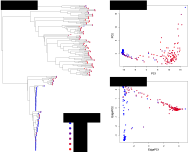
\includegraphics[width=\linewidth]{squash_edgepca.pdf}
    \begin{subfigure}{0pt}
        \phantomcaption
        \label{fig:squash_edgepca:sub:squash}
    \end{subfigure}
    \begin{subfigure}{0pt}
        \phantomcaption
        \label{fig:squash_edgepca:sub:pca}
    \end{subfigure}
    \begin{subfigure}{0pt}
        \phantomcaption
        \label{fig:squash_edgepca:sub:epca}
    \end{subfigure}
    \caption[Existing analysis methods on the BV dataset]{
        \textbf{Existing analysis methods on the BV dataset.}
        We applied \subref{fig:squash_edgepca:sub:squash} Squash Clustering,
        \subref{fig:squash_edgepca:sub:pca} PCA on the pairwise KR distance matrix between samples,
        and \subref{fig:squash_edgepca:sub:epca} Edge PCA,
        using the \acf{BV} dataset \cite{Srinivasan2012}.
        The Subfigures are recalculations of Figure~1(A) of \cite{Srinivasan2012},
        and Figures~4 and 3 of \cite{Matsen2011b}, respectively.
        All Subfigures represent samples as colored dots according to their respective Nugent score,
        which indicates the severeness of the \ac{BV} infection of the samples/patients.
%         In \subref{fig:squash_edgepca:sub:squash}, we added coloring to the samples (tips) of the cluster tree for convenience.
        See \secref{ch:Foundations:sec:PhylogeneticPlacement:sub:ExistingMethods} for a description of the methods,
        and \appref{supp:sec:DetailsEmpiricalDatasets:sub:BV} for details on the dataset.
    }
    \label{fig:squash_edgepca}
\end{figure}

Furthermore, depending on the data and research question at hand,
the KR distance is not always the best measure of sample similarity.
As explained in \secref{ch:Foundations:sec:PhylogeneticPlacement:sub:PlacementProcessing},
edge imbalances can often reveal more subtle differences between samples than edge masses.
Thus, for some datasets, it might make sense to use a distance based on edge imbalances instead.

To further illustrate this, \figref{fig:squash_edgepca:sub:pca} shows
the result of a standard principal component analysis (PCA) \cite{Pearson1901,Jolliffe2002}
on the pairwise KR distance matrix of the \acf{BV} dataset \cite{Srinivasan2012} that we used before.
On the left hand side of the figure, the blue samples,
representing healthy women with a low Nugent score, form a dense cluster.
Towards the right hand side however, the red samples, which belong to sick patients, are spread over the rest of the graph.
As Squash Clustering also uses the KR distance, the same pattern can be observed in its resulting clustering tree,
as shown in \figref{fig:squash_edgepca:sub:squash}:
The bottom half of the clustering tree, containing mainly healthy (blue) samples, has short branches,
which correspond to the dense blue region in \figref{fig:squash_edgepca:sub:pca}.
At the same time, the top half, with mostly samples from sick (red) patients, has many long branches,
corresponding to the scattered red region in \figref{fig:squash_edgepca:sub:pca}.
Thus, Squash Clustering represents equivalent information to a standard PCA on this dataset.
It thus ``suffers'' from the same shortcomings that Edge PCA is solving by using mass imbalance instead
(see \secref{ch:Foundations:sec:PhylogeneticPlacement:sub:ExistingMethods:par:EdgePCA}).
This can be seen in \figref{fig:squash_edgepca:sub:epca}, which shows the result of Edge PCA on the dataset.
There, the healthy (blue) samples clearly separate
into two groups for the two dominant \taxonname{Lactobacillus} clades in healthy patients,
which is due to the edge imbalances resolving smaller differences between the placements on nearby clades in this dataset.
Hence, for this dataset, instead of using a distance based on edge masses such as the KR distance,
edge imbalances should be used to measure distances between samples.

% ######################################################################################################################
%         Methods and Implementation
% ######################################################################################################################

\section{Methods and Implementation}
\label{ch:Clustering:sec:Methods}

We here propose two variants of $k$-means clustering \cite{Steinhaus1956,Macqueen1967},
which we call \emph{Phylogenetic $k$-means}, and \emph{Imbalance $k$-means}, respectively.
They are clustering methods for phylogenetic placement of a set of metagenomic sequence samples,
and address the issues described above.
Note that these methods are clustering samples, and not single sequences \cite{Kelley2010}.
Both methods produce a predefined number of clusters, and hence are able to work with arbitrarily large datasets.
Phylogenetic $k$-means uses the KR distance to assess sample similarity, that is, it uses edge masses,
while Imbalance $k$-means uses edge imbalances instead.

The methods take as input a set of $n$ samples, each consisting of their \acfp{QS} placed on a fixed \acf{RT}.
They then assign the samples to $k$ clusters, each represented by a cluster \emph{centroid}
that describes the average placement mass distribution of the samples assigned to it.
We later also discuss how to chose a reasonable value for $k$.

% ======================================================================================================================
%     Phylogenetic k-means
% ======================================================================================================================

% PDF bookmarks do not accept the $k$ math mode, so make it use the letter instead.
\subsection{Phylogenetic \texorpdfstring{$k$-means}{k-means}}
\label{ch:Clustering:sec:Methods:sub:PhylogeneticKmeans}

Phylogenetic $k$-means employs the KR distance (see \secref{ch:Foundations:sec:PhylogeneticPlacement:sub:Distances:par:KR})
and hence yields results that are consistent with the clustering tree of Squash Clustering.
% but it yields a predefined number of $k$ clusters.

% ----------------------------------------------------------------------------------------------------------------------
%     Algorithm
% ----------------------------------------------------------------------------------------------------------------------

\paragraph{Algorithm}
\label{ch:Clustering:sec:Methods:sub:PhylogeneticKmeans:par:Algorithm}

% The underlying idea is to assign each of the $n$ samples to one of $k$ cluster centroids,
% where each centroid represents the average mass distribution of all samples assigned to it.

The input samples and the cluster centroids are of the same data type,
namely, they are mass distributions on a fixed \ac{RT}.
It is thus possible to calculate the KR distances between samples and centroids,
and to calculate their average mass distributions by \emph{squashing},
as described in \secref{ch:Foundations:sec:PhylogeneticPlacement:sub:PlacementProcessing:par:EdgeMasses}.

The objective is then to find an assignment of the $n$ samples into $k$ clusters
that minimizes the total distance between each sample and the cluster centroid it is assigned to,
measured as the KR distance between them.
That is, for $k$ clusters, each represented by a set $A_k$ of samples assigned to it, and its centroid $C_k$,
the objective is to find

\begin{equation}
    \label{ch:Clustering:eq:KmeansObjective}
    \hat{A} ~=~ \argmin_A \sum_{i=1}^{k} \sum_{s \in A_i} \mbox{KR}( s, C_i )
\end{equation}

% Keep in mind that each sample in the assignments $A_k$ and each centroid $C_k$
% are placement mass distributions on the \ac{RT}, between which the KR distance can be calculated.
The optimal solution $\hat{A}$ for the assignment of samples to clusters can be found via a brute-force search.
However, the number of possible assignments of $n$ samples to $k$ clusters
is given by the Stirling partition number $S(n,k)$ \cite{Graham1989a},
which is too large for any realistic dataset.

Hence, our implementation follows the Lloyd-Forgy algorithm \cite{Lloyd1982,Forgy1965},
which is the standard heuristical method to solve the $k$-means problem.
It iteratively improves the assignments $A$ and the centroids $C$ in two alternating steps,
as shown in \algref{algo:kmeans}.

% \todo{maybe remove space later again:}
% \vspace*{1em}
\begin{algorithm}
\caption{Phylogenetic $k$-means}\label{algo:kmeans}
\begin{algorithmic}[1]
    \State initialize $k$ \textit{Centroids}
    \While{not converged}
        \State assign each \textit{Sample} to nearest \textit{Centroid} ($A$)
        \State update \textit{Centroids} as mass averages of their \textit{Samples} ($C$)
    \EndWhile
    \State \textbf{return} \textit{Assignments} $A$ and \textit{Centroids} $C$
\end{algorithmic}
\end{algorithm}

By default, we use the $k$-means++ initialization algorithm \cite{Arthur2007} to obtain an initial set of $k$ centroids.
It works by subsequent random selection of samples to be used as initial centroids,
until $k$ centroids have been selected.
In each step, the probability of selecting a sample is
proportional to its squared distance to the nearest already selected sample.
Hence, centroids are preferably selected that are far away from each other.
An alternative initialization is to select samples as initial clusters entirely at random.
This is however more likely to yield sub-optimal clusterings \cite{Kanungo2003}.

Then, each sample is assigned to its nearest centroid, using the KR distance. %for example the KR or NH distance.
Lastly, the centroids are updated to represent
the average mass distribution of all samples that are currently assigned to them.
This iterative process alternates between improving the assignments and the centroids.
Thus, the main difference to normal $k$-means in the $\mathbb{R}^d$ is the use of phylogenetic information:
Instead of euclidean distances on vectors, we use the KR distance,
and instead of averaging vectors to obtain centroids, we use the average mass distribution.

The process is repeated until it converges,
that is, the cluster assignments do not change any more between subsequent iterations,
or until a maximum number of iterations have been executed.
% The second stopping criterion makes sure that the algorithm terminates even with non-convergent datasets.
This second stopping criterion is added to avoid the super-polynomial worst case running time of $k$-means,
which however almost never occurs in practice \cite{Bottou1995,Arthur2006}.

The result of the algorithm is an assignment of each sample to one of the $k$ clusters.
As the algorithm relies on the KR distance, it clusters samples with similar relative abundances.
The cluster centroids can be visualized as trees with a mass distribution,
analogous to how Squash Clustering visualizes inner nodes of the clustering tree.
That is, each centroid can be represented as the average mass distribution of the samples that were assigned to it.
This allows to inspect the centroids and thus to interpret how the samples were clustered.
% For instance, the diversity and taxonomic assignment of the centroids represents the corresponding sets of samples.
Examples of this are shown in \figref{fig:centroids}.

% ----------------------------------------------------------------------------------------------------------------------
%     Algorithmic Improvements
% ----------------------------------------------------------------------------------------------------------------------

\paragraph{Algorithmic Improvements}
\label{ch:Clustering:sec:Methods:sub:PhylogeneticKmeans:par:AlgorithmicImprovements}

In each assignment step of the algorithm, distances from all samples to all centroids are calculated,
which has a time complexity of $\mathcal{O}(n \cdot k)$.
In order to accelerate this step, we can apply branch binning
as introduced in \secref{ch:Foundations:sec:PhylogeneticPlacement:sub:PlacementProcessing:par:EdgeMasses}.
For the \ac{BV} dataset, we found that even using just \num{2} bins per edge does not alter the cluster assignments.
Branch binning reduces the number of mass points that have to be accessed in memory during KR distance calculations;
however, the costs for tree traversals remain.
Thus, we observed a maximal speedup of 75\% when using one bin per branch,
see \tabref{tab:hmp_binning_error} for details.
Intermediate binning strategies are also possible:
instead of binning all masses of the input samples, just the centroid masses can be binned.

% even binning to \num{1} bin,
% that is, combining all placement masses on a branch into one point,
% changes the cluster assignment of only \num{2} of {220} samples
% -- both of which were near the border between two clusters.
% The main bottleneck in the computation however seems to be
% the random memory access to the edges and per-edge masses induced by the tree traversals
% so that binning does not yield substantial speedups.
% In our tests, summarizing all masses in one bin per branch resulted in a speedup of around 75\%,

Furthermore, during the execution of the algorithm, empty clusters can occur,
for example, if $k$ is greater than the number of natural clusters in the data.
Although this problem did not occur in our tests, we implemented the following solution:
First, find the cluster with the highest variance.
Then, choose the sample of that cluster that is furthest from its centroid,
and assign it to the empty cluster instead.
This process is repeated if multiple empty clusters occur at once.

% ======================================================================================================================
%         Imbalance k-means
% ======================================================================================================================

% PDF bookmarks do not accept the $k$ math mode, so make it use the letter instead.
\subsection{Imbalance \texorpdfstring{$k$-means}{k-means}}
\label{ch:Clustering:sec:Methods:sub:ImbalanceKmeans}

We further propose \emph{Imbalance $k$-means},
which is a variant of $k$-means that makes use of the edge imbalance transformation
(see \secref{ch:Foundations:sec:PhylogeneticPlacement:sub:PlacementProcessing:par:EdgeImbalances}),
and thus takes the clades of the reference tree into account.
In order to quantify the difference in imbalances between two samples,
we use the euclidean distance between their imbalance vectors (that is, rows of the imbalance matrix).
This is a suitable distance measure,
as the imbalances implicitly capture the tree topology as well as the placement mass distributions.
As a consequence, the expensive tree traversals required for Phylogenetic $k$-means are not necessary for the calculations.
The algorithm takes the edge imbalance matrix of normalized samples as input,
% as shown in \figref{fig:imbalance:sub:Matrices},
and performs a standard euclidean $k$-means clustering following the Lloyd-Forgy algorithm \cite{Lloyd1982,Forgy1965}.
% As there is no apparent phylogenetically informative distance measure between imbalance vectors,
% we use euclidean distance instead.
% This also allows to calculated centroids as simple vector averages.

This variant of $k$-means tends to find clusters that are consistent with the results of Edge PCA,
as both use the same input data and both operate in euclidean space. %as well as the same distance measure.
Furthermore, as the method does not need to calculate KR distances,
and thus neither involves tree traversals nor needs to consider each placement location (or bins of those) separately,
it is several orders of magnitude faster than Phylogenetic $k$-means.
For example, on the \ac{HMP} dataset (see \appref{supp:sec:DetailsEmpiricalDatasets:sub:HMP}),
it runs in mere seconds, instead of several hours needed for Phylogenetic $k$-means;
see Section \secref{ch:Clustering:sec:Results:sub:Performance} for details.

% ======================================================================================================================
%     Finding k
% ======================================================================================================================

\subsection{Finding appropriate values for \texorpdfstring{$k$}{k}}
\label{ch:Clustering:sec:Methods:sub:FindingK}

A commonly criticized downside of $k$-means clustering in general is
that the number of clusters $k$ is an input parameter to the algorithm.
Hence, a key question is how to select an appropriate $k$
that reflects the number of ``natural'' clusters in the data.
There exist various suggestions in the literature
\cite{Thorndike1953,Rousseeuw1987,Bischof1999,Pelleg2000,Tibshirani2001,Hamerly2004}.
% See also: https://stackoverflow.com/a/1793572/4184258 and
% http://www.sthda.com/english/articles/29-cluster-validation-essentials/96-determining-the-optimal-number-of-clusters-3-must-know-methods/

We evaluated the Elbow method \cite{Thorndike1953},
which is a straight forward method that yielded reasonable results for our test datasets.
It works by plotting the cluster variance,
that is, the average squared distance of the samples to their assigned cluster centroids,
for different values of $k$.
On the one hand, for low values of $k$, many samples exhibit a large distance to their assigned centroid,
% the distances from samples to their assigned centroids are relatively
inducing a high variance.
On the other hand, higher values of $k$ further split the clusters and hence reduce the variance.
% and slightly reduce this distance by further splitting clusters.
Thus, at a given point, increasing $k$ only yields a marginal change in variance.
If the data has a natural number of clusters, the corresponding $k$ at this point produces an angle in the plot,
called the \emph{elbow}.
Thus, the presence of an elbow in the variance plot indicates reasonable values for $k$.

Additionally, for a quantitative evaluation of the clusterings,
we used the $k$ that arose from the number of distinct categories or labels based on the available meta-data for the data.
% that is, the number of distinct categories our data is known to belong to.
For example, the samples of the \ac{HMP} dataset are labeled with \num{18} distinct body sites,
describing where each sample was taken from, c.f.~\figref{fig:hmp_kmeans_all_18}.

% ######################################################################################################################
%         Results
% ######################################################################################################################

\section{Evaluation and Results}
\label{ch:Clustering:sec:Results}

We here evaluate the two $k$-means variants in terms of their clustering accuracy and performance.
We used the \acf{BV} dataset (see \appref{supp:sec:DetailsEmpiricalDatasets:sub:BV} for details)
as an example of a small dataset to which methods such as Squash Clustering \cite{Matsen2011a}
are still applicable for comparison,
and the \acf{HMP} dataset (see \appref{supp:sec:DetailsEmpiricalDatasets:sub:HMP})
to showcase that our methods scale to datasets that are too large for existing methods.

% ======================================================================================================================
%     BV Dataset
% ======================================================================================================================

\subsection{BV Dataset}
\label{ch:Clustering:sec:Results:sub:BVDataset}

We placed the samples of the \ac{BV} dataset \cite{Srinivasan2012}
on the re-inferred reference tree of their original reference sequences
to test whether our methods work as expected.
To this end, we ran both Phylogenetic $k$-means and Imbalance $k$-means on the \ac{BV} dataset,
and compare the results to the existing analysis of the data in \cite{Srinivasan2012} and \cite{Matsen2011a}.
We chose $k:=3$, inspired by the findings of \cite{Srinivasan2012}.
There, they distinguish between subjects affected by Bacterial Vaginosis and healthy subjects,
and further separate the healthy ones into two categories depending on the dominating clade in the vaginal microbiome,
which is either \taxonname{Lactobacillus iners} or \taxonname{Lactobacillus crispatus}.
Any choice of $k > 3$ would simply result in smaller, more fine-grained clusters,
but not change the general findings of these experiments.
The number of clusters is also evaluated using the Elbow method later in \secref{ch:Clustering:sec:Results:sub:ElbowMethod}.

For each of the \num{220} samples of the dataset, we hence obtained two cluster assignments:
First, by using Phylogenetic $k$-means, we obtained the cluster assignment \emph{PKM}.
Second, by using Imbalance $k$-means, we obtained assignment \emph{IKM}.
In the following figures, the samples are represented by colored circles:
red, green, and blue show the cluster assignments \emph{PKM},
while purple, orange, and gray show the cluster assignments \emph{IKM}.
We use two different color sets for the two methods, in order to make them distinguishable at first glance.
Note that the mapping of colors to clusters is arbitrary and depends on the random initialization of the algorithm.

We then conducted Squash Clustering and Edge PCA (\secref{ch:Foundations:sec:PhylogeneticPlacement:sub:ExistingMethods})
on the dataset, thereby reproducing results of previous studies,
as well as two alternative dimensionality reduction methods.
This allows for a direct comparison between our novel and the existing methods.

% The figure shows the results of Squash Clustering, Edge PCA, and two alternative dimensionality reduction methods,
% colorized by the cluster assignments \emph{PKM} of Phylogenetic $k$-means (in red, green, and blue)
% and \emph{IKM} of the Imbalance $k$-means (in purple, orange, and gray), respectively.

% ----------------------------------------------------------------------------------------------------------------------
%     Squash Clustering
% ----------------------------------------------------------------------------------------------------------------------

\paragraph{Comparison to Squash Clustering}
\label{ch:Clustering:sec:Results:sub:BVDataset:par:SquashClustering}

\begin{figure}[p]
    \centering
    \includegraphics[width=\linewidth]{cluster_kmeans_trees.pdf}
    \begin{subfigure}{0pt}
        \phantomcaption
        \label{fig:cluster_kmeans_trees:sub:mass_tree}
    \end{subfigure}
    \begin{subfigure}{0pt}
        \phantomcaption
        \label{fig:cluster_kmeans_trees:sub:imbalance_tree}
    \end{subfigure}
    \caption[Comparison of $k$-means clustering to Squash Clustering]{
        \textbf{Comparison of $k$-means clustering to Squash Clustering.}
        We applied Squash Clustering to the \ac{BV} dataset \cite{Srinivasan2012},
        to compare it to the assignments obtained from our $k$-means variants.
        % in order to compare them to existing methods.
%         See \cite{Srinivasan2012} for details of the dataset and its interpretation.
%         We chose $k:=3$, as this best fits the features of the dataset.
        % Sub (A)
        \subref{fig:cluster_kmeans_trees:sub:mass_tree}
        Hierarchical cluster tree of the samples, using Squash Clustering.
        The tree is a recalculation of Figure~1(A) of \cite{Srinivasan2012}.
        Each leaf represents a sample; branch lengths are KR distances.
        We added color coding for the samples, using \emph{PKM}.
        The lower half of red samples are mostly healthy subjects,
        while the green and blue upper half are patients affected by Bacterial Vaginosis.
        % Sub (B)
        \subref{fig:cluster_kmeans_trees:sub:imbalance_tree}
        The same tree, but annotated by \emph{IKM}.
        The tree is flipped horizontally for ease of comparison.
        The healthy subjects are split into two sub-classes,
        discriminated by the dominating species in their vaginal microbiome:
        orange and purple represent samples were \taxonname{Lactobacillus iners} and \taxonname{Lactobacillus crispatus}
        dominate the microbiome, respectively.
        The patients mostly affected by BV are clustered in gray.
    }
    \label{fig:cluster_kmeans_trees}
\end{figure}

The comparison of our $k$-means clustering assignments to Squash Clustering is shown in \figref{fig:cluster_kmeans_trees}.
As can be seen in \figref{fig:cluster_kmeans_trees:sub:mass_tree}, Squash Clustering as well as
Phylogenetic $k$-means can distinguish healthy subjects from those affected by Bacterial Vaginosis.
Healthy subjects constitute the lower part of the cluster tree.
They have shorter branches between each other, indicating the smaller KR distance between them,
which is a result of the dominance of \taxonname{Lactobacillus} in healthy subjects.
The same clusters are found by Phylogenetic $k$-means:
As it uses the KR distance, it assigns all healthy subjects to one cluster (shown in red),
which is consistent with the short cluster tree branches in \figref{fig:cluster_kmeans_trees:sub:mass_tree}.
The green and blue clusters are mostly the subjects affected by the disease.

In \figref{fig:cluster_kmeans_trees:sub:imbalance_tree}, we compare Squash Clustering to Imbalance $k$-means.
Here, the distinction between the two \taxonname{Lactobacillus} clades
can be seen by the purple and orange cluster assignments.
The cluster tree also separates those clusters into two clades.
The separate small group of orange samples above the purple clade is an artifact of the tree visualization (ladderization),
and actually is close to the other orange samples below.
The diseased subjects are all assigned to the gray cluster, represented by the upper half of the cluster tree.
It is apparent that both methods separate the same samples from each other.

% ----------------------------------------------------------------------------------------------------------------------
%     Edge PCA
% ----------------------------------------------------------------------------------------------------------------------

\paragraph{Comparison to Edge PCA}
\label{ch:Clustering:sec:Results:sub:BVDataset:par:EdgePCA}

\begin{figure}[p]
    \centering
    \includegraphics[width=\linewidth]{kmeans_all.pdf}
    \begin{subfigure}{0pt}
        \phantomcaption
        \label{fig:kmeans_all:sub:mds_em}
    \end{subfigure}
    \begin{subfigure}{0pt}
        \phantomcaption
        \label{fig:kmeans_all:sub:mds_ei}
    \end{subfigure}
    \begin{subfigure}{0pt}
        \phantomcaption
        \label{fig:kmeans_all:sub:mds_ns}
    \end{subfigure}
    \begin{subfigure}{0pt}
        \phantomcaption
        \label{fig:kmeans_all:sub:pca_em}
    \end{subfigure}
    \begin{subfigure}{0pt}
        \phantomcaption
        \label{fig:kmeans_all:sub:pca_ei}
    \end{subfigure}
    \begin{subfigure}{0pt}
        \phantomcaption
        \label{fig:kmeans_all:sub:pca_ns}
    \end{subfigure}
    \begin{subfigure}{0pt}
        \phantomcaption
        \label{fig:kmeans_all:sub:epca_em}
    \end{subfigure}
    \begin{subfigure}{0pt}
        \phantomcaption
        \label{fig:kmeans_all:sub:epca_ei}
    \end{subfigure}
    \begin{subfigure}{0pt}
        \phantomcaption
        \label{fig:kmeans_all:sub:epca_ns}
    \end{subfigure}
    \caption[Comparison of $k$-means clustering to MDS, PCA, and Edge PCA]{
        \textbf{Comparison of $k$-means clustering to MDS, PCA, and Edge PCA.}
        Here, we show the dimensionality reduction methods MDS, PCA, and Edge PCA (one per row) on the \ac{BV} dataset.
        MDS and PCA were calculated on the pairwise KR distance matrix of the samples,
        Edge PCA was calculated using the placements on the re-inferred \ac{RT} of the original publication \cite{Srinivasan2012}.
        The plots are colored by the cluster assignments \emph{PKM} and \emph{IKM}
        as found by our $k$-means variants (first two columns), and by the Nugent score of the samples (third column).
        The Nugent score is included to allow comparison of the health status of patients with the clustering results.
        \subref{fig:kmeans_all:sub:pca_ns} and \subref{fig:kmeans_all:sub:epca_ns} are recalculations of
        Figures~4 and 3 of \cite{Matsen2011b}, respectively.
    }
    \label{fig:kmeans_all}
\end{figure}

In \figref{fig:kmeans_all}, we compare the assignments obtained from our $k$-means variants
to several dimensionality reduction methods, such as Edge PCA.
The figure reveals additional details about how the $k$-means method works,
that is, which samples are assigned to the same cluster.

The first row of \figref{fig:kmeans_all} shows the result of
\acf{MDS} of the pairwise KR distance matrix between the samples.
\ac{MDS} \cite{Mardia1978,Krzanowski1994,Everitt2010} is a dimensionality reduction method that
can be used for visualizing levels of similarity between data points.
Given a pairwise distance matrix, it finds an embedding into lower dimensions (in this case, \num{2} dimensions)
that preserves higher dimensional distances as well as possible.

The distinguishing features between the green and the blue cluster
are not apparent in the Squash cluster tree in \figref{fig:cluster_kmeans_trees:sub:mass_tree}.
This can however be seen in \figref{fig:kmeans_all:sub:mds_em}, which shows the \ac{MDS} plot colored by \emph{PKM}.
Here, the red cluster forms a dense region, which is in agreement with the short branch lengths
in the cluster tree of \figref{fig:cluster_kmeans_trees:sub:mass_tree}.
At the same time, the green and blue cluster are separated in the \ac{MDS} plot,
but form a coherent region of low density,
indicating that $k:=3$ might be too large when applying Phylogenetic $k$-means to this dataset.
That is, the actual clustering just distinguishes healthy from sick patients (c.\,f.~\figref{fig:elbows}),
meaning that \num{2} dimensions might also suffice here.
% which, albeit not well separated from each other, indicate groups of samples with lower KR distance between each other.
Although the separation between green and blue samples is smooth,
it shows that Phylogenetic $k$-means finds clusters based on KR distance between samples,
and thus yields results consistent with Squash Clustering and \ac{MDS}.

A similar visualization of the pairwise KR distances is shown in the second row of \figref{fig:kmeans_all},
where we applied standard \acf{PCA} \cite{Krzanowski1994,Everitt2010} to the pairwise KR distance matrix
by interpreting it as a data matrix.
Although it is mathematically sound, the direct application of \ac{PCA} to a distance matrix lacks a simple interpretation,
which was previously used to motivate Edge PCA
(c.\,f.~\secref{ch:Foundations:sec:PhylogeneticPlacement:sub:ExistingMethods:par:EdgePCA}).
Still, this can be seen as a visualization of the distances that helps understanding our methods.

For example, in \figref{fig:kmeans_all:sub:pca_em},
% It is a recalculation of Figure~4 in the preprint \cite{Matsen2011b},
% which did not appear in the final published version \cite{Matsen2011a}.
% It is a recalculation of Figure~4 of \cite{Matsen2011b}.
% but can also be found at \cite{MatsenEdgePCA}.
which shows the PCA plot colored by \emph{PKM}, the red cluster again is clearly separated from the rest.
This time however, the distinction between the green and the blue cluster
is not as apparent as in \figref{fig:kmeans_all:sub:mds_em}.

Furthermore, \figref{fig:kmeans_all:sub:mds_ei} and \subref{fig:kmeans_all:sub:pca_ei} show the MDS and the PCA plot,
respectively, this time colored by \emph{IKM}.
Here, the purple cluster found by Imbalance $k$-means forms a dense cluster of close-by samples on the left of the plots,
which is in accordance with the short branch lengths
of this cluster as shown in the clustering tree in \figref{fig:cluster_kmeans_trees:sub:imbalance_tree}.
The orange cluster is slightly more spread out in the plots,
which again can be seen by the longer branch lengths in \figref{fig:cluster_kmeans_trees:sub:imbalance_tree}.

Finally, we applied Edge PCA to the samples, as shown in the last row of \figref{fig:kmeans_all}.
In particular, \figref{fig:kmeans_all:sub:epca_ei} compares Imbalance $k$-means to Edge PCA
by coloring the plot using \emph{IKM}.
% The plot is a recalculation of Figure~3 of \cite{Matsen2011b}, which also appeared in Figure~6 in \cite{Matsen2011a}
% and Figure~3 in \cite{Srinivasan2012},
Because both methods work on edge imbalances, they group the data in the same way, and are thus consistent with each other.
That is, they clearly separate the two healthy groups and the diseased one from each other.
Edge PCA forms a plot with three corners, which are colored by the three Imbalance $k$-means cluster assignments.

% ----------------------------------------------------------------------------------------------------------------------
%     Cluster Centroids
% ----------------------------------------------------------------------------------------------------------------------

\paragraph{Cluster Centroids}
\label{ch:Clustering:sec:Results:sub:BVDataset:par:ClusterCentroids}

As mentioned before, an advantage of using phylogenetic placements as input to our $k$-means clustering methods
is the ability to visualize cluster centroids by showing the average mass distribution
of the samples assigned to them on the underlying \acf{RT}.
In Phylogenetic $k$-means, the mass distributions of the centroids are already part of the algorithm,
as they are needed for calculating the KR distances between samples and centroids.
In Imbalance $k$-means however, the placement data is used in form of edge imbalances instead of masses.
Still, after convergence of the algorithm, the per-centroid average mass can be calculated from the input samples
and again visualized on the \ac{RT}.

\begin{figure}[!tb]
    \centering
    \includegraphics[width=\linewidth]{centroids.pdf}
    \begin{subfigure}{0pt}
        \phantomcaption
        \label{fig:centroids:sub:red}
    \end{subfigure}
    \begin{subfigure}{0pt}
        \phantomcaption
        \label{fig:centroids:sub:green}
    \end{subfigure}
    \begin{subfigure}{0pt}
        \phantomcaption
        \label{fig:centroids:sub:blue}
    \end{subfigure}
    \begin{subfigure}{0pt}
        \phantomcaption
        \label{fig:centroids:sub:purple}
    \end{subfigure}
    \begin{subfigure}{0pt}
        \phantomcaption
        \label{fig:centroids:sub:orange}
    \end{subfigure}
    \begin{subfigure}{0pt}
        \phantomcaption
        \label{fig:centroids:sub:gray}
    \end{subfigure}
    \caption[Example of $k$-means cluster centroids visualization]{
        % In this figure, I assume that the reader is already familiar with the characteristics of the dataset.
        % No need to repeat everything over again...
        \textbf{Example of $k$-means cluster centroids visualization.}
        Here we show the cluster centroids as found by our $k$-means variants using the \ac{BV} dataset,
        visualized on the reference tree via color coding.
        The cluster assignments are the same as in \figref{fig:cluster_kmeans_trees} and \figref{fig:kmeans_all};
        the first row show the three clusters found by Phylogenetic $k$-means,
        the second row the clusters found by Imbalance $k$-means.
        Each tree represents one centroid around which the samples were clustered,
        that is, it shows the combined masses of the samples that were assigned to that cluster.
        The edges are colored relative to each other, using a linear scaling of
        light blue (no mass), purple (half of the maximal mass) and black (maximal mass).
        The two \taxonname{Lactobacillus} clades are marked with black arcs on the left of the trees.
    }
    \label{fig:centroids}
\end{figure}

Examples of this are shown in \figref{fig:centroids},
for both sample assignments \emph{PKM} (first row) and \emph{IKM} (second row) of the \ac{BV} dataset.
As explained above, the samples can be split into three groups:
The diseased subjects, which have placement mass in various parts of the tree,
as well as two groups of healthy subjects, with placement mass in one of two \taxonname{Lactobacillus} clades,
marked with black arcs in \figref{fig:centroids}.
This grouping is also clearly visible in the trees.
The red cluster in \subref{fig:centroids:sub:red} for example represents all healthy subjects;
thus, most of its mass is located in the two \taxonname{Lactobacillus} clades.
The purple and orange clusters in \subref{fig:centroids:sub:purple} and \subref{fig:centroids:sub:orange}
on the other hand show a difference in placement mass between those clades.
Furthermore, the placement mass of the gray cluster in \subref{fig:centroids:sub:gray} is mostly
a combination of the masses of the green and blue cluster in \subref{fig:centroids:sub:green} and \subref{fig:centroids:sub:blue},
all of which represent diseased subjects.
These observations are in accordance with the previous findings above,
and further support that our methods yield results that are in agreement with existing methods.
% In summary, our novel $k$-means variants find clusters that are in agreement with existing methods.

% ======================================================================================================================
%     HMP Dataset
% ======================================================================================================================

\subsection{HMP Dataset}
\label{ch:Clustering:sec:Results:sub:HMPDataset}

The \acf{HMP} dataset \cite{Huttenhower2012,Methe2012} (see \appref{supp:sec:DetailsEmpiricalDatasets:sub:HMP} for details)
is used here as an example to show that our method scales to large datasets.
To this end, we used the unconstrained \taxonname{Bacteria} \ac{RT} with \num{1 914} taxa
obtained from our \ac{PhAT} method, see \secref{ch:AutomaticTrees:sec:Evaluation:sub:ReferenceTreeSetup} for details.
% as provided by our Automatic Reference Tree method \cite{Czech2018}.
The tree represents a broad taxonomic range of \taxonname{Bacteria},
that is, the sequences were \emph{not} explicitly selected for the \ac{HMP} dataset,
in order to test the robustness of our clustering methods.
We then placed the \num{9 192} samples of the \ac{HMP} dataset with a total of \num{118 701 818} sequences on that tree,
and calculated Phylogenetic and Imbalance $k$-means on the samples.

The freely available meta-data for the \ac{HMP} dataset labels each sample by the body site were it was taken from.
As there are \num{18} different body site labels, we used $k:=18$.
The resulting clustering assignments are shown in \figref{fig:hmp_kmeans_all_18}.
Furthermore, in \figref{fig:hmp_kmeans_all_8},
we show a clustering of this dataset into $k:=8$ broader body site groups
to exemplify the effect of using different values of $k$.
See \tabref{tab:hmp_data_overview} for the grouping of the original body site labels.
The effect of $k$ on the clustering results is further explored by using the Elbow method,
as described later in \secref{ch:Clustering:sec:Results:sub:ElbowMethod}.
% that is, using the constrained Bacterial tree as well as Imbalance $k$-means.

\begin{figure}[hpbt]
    \centering
    \includegraphics[width=\linewidth]{hmp_kmeans_all_18.pdf}
    \begin{subfigure}{0pt}
        \phantomcaption
        \label{fig:hmp_kmeans_all_18:sub:em_unconstr}
    \end{subfigure}
    \begin{subfigure}{0pt}
        \phantomcaption
        \label{fig:hmp_kmeans_all_18:sub:ei_unconstr}
    \end{subfigure}
    \caption[$k$-means cluster assignments of the \acs{HMP} dataset with $k:=18$]{
        \textbf{$k$-means cluster assignments of the \acs{HMP} dataset with $k:=18$.}
        Here, we show the cluster assignments as yielded by
        \subref{fig:hmp_kmeans_all_18:sub:em_unconstr} Phylogenetic $k$-means and
        \subref{fig:hmp_kmeans_all_18:sub:ei_unconstr} Imbalance $k$-means on the \ac{HMP} dataset.
        We used $k:=18$, which is the number of body site labels in the dataset,
        in order to compare the clusterings to this ``ground truth''.
        Each row represents a body site; each column one of the 18 clusters found by the algorithm.
        We also show a translation of the body site labels into the corresponding body regions.
        The color values indicate how many samples of a body site are assigned to each cluster.
        Similar body sites are clearly grouped together in coherent blocks, indicated by darker colors.
        For example, the stool samples are split into two clusters (topmost row),
        while the three vaginal sites are all put into one cluster (rightmost column).
        However, the algorithm cannot always distinguish between nearby body sites,
        as can be seen from the fuzziness of the clusters of oral samples.
%         Lastly, the figure also lists how the body site labels were aggregated into coarse regions
%         as used in \figref{fig:hmp_kmeans_all_8}.
    }
    \label{fig:hmp_kmeans_all_18}
\end{figure}

\begin{figure}[hpbt]
    \centering
    \includegraphics[width=0.6\linewidth]{hmp_kmeans_all_8.pdf}
    \begin{subfigure}{0pt}
        \phantomcaption
        \label{fig:hmp_kmeans_all_8:sub:em_unconstr}
    \end{subfigure}
    \begin{subfigure}{0pt}
        \phantomcaption
        \label{fig:hmp_kmeans_all_8:sub:ei_unconstr}
    \end{subfigure}
    \caption[$k$-means cluster assignments of the \acs{HMP} dataset with $k:=8$]{
        \textbf{$k$-means cluster assignments of the \acs{HMP} dataset with $k:=8$.}
        Here, we again show the cluster assignments as yielded by
        \subref{fig:hmp_kmeans_all_8:sub:em_unconstr} Phylogenetic $k$-means and
        \subref{fig:hmp_kmeans_all_8:sub:ei_unconstr} Imbalance $k$-means on the \ac{HMP} dataset,
        but with $k$ being set to 8, instead of $k:=18$ as in \figref{fig:hmp_kmeans_all_18}.
        These \num{8} clusters are based on an aggregation of the original body site labels into groups,
        as shown in \tabref{tab:hmp_data_overview}.
%         for the list of how the original body site labels were aggregated.
        %for the cluster assignment where $k$ is set to the original number of labels;
        Each row represents a body group; each column one of the \num{8} clusters found by the algorithm.
%         The color values indicate how many samples of a body site were assigned to each cluster.
        Some of the body sites are again clearly separated,
        while particularly the samples from the oral region are distributed over different clusters.
%         This might be due to %the broad reference tree not being able to resolve the fine details between these samples,
%         but might also indicate a
%         homogeneity of the oral samples.
    }
    \label{fig:hmp_kmeans_all_8}
\end{figure}

% Ideally, each cluster would contain only samples from the same body site.
Ideally, all samples from one body site would be assigned to the same cluster,
hence forming a diagonal in the plots of \figref{fig:hmp_kmeans_all_18} and \figref{fig:hmp_kmeans_all_8}.
However, as there are several nearby body sites, which share a large fraction of their microbiome \cite{Huttenhower2012},
we do not expect a perfect clustering.
Furthermore, we used a broad reference tree that might not be able to resolve details in some clades.
% which was originally meant only for a first classification of sequences (see above).
% Thus, the tree does not particularly suit the dataset well.
Nonetheless, the clustering is reasonable, which indicates a robustness against the exact choice of reference taxa.
% and can thus be used for distinguishing among samples.

The plots of the two $k$-means variants generally exhibit similar characteristics in \figref{fig:hmp_kmeans_all_18}.
Most prominently, the stool and vaginal samples are clearly clustered into coherent blocks in both variants.
There are however also some differences.
For example, the samples from the body surface (arm, nose, and ear)
form two relatively dense clusters (columns) in \figref{fig:hmp_kmeans_all_18:sub:em_unconstr},
whereas those sites are spread across four or five clusters in \figref{fig:hmp_kmeans_all_18:sub:ei_unconstr}.
% In general however, these samples form two blocks of cluster columns in both plots.
On the other hand, the mouth samples are more densely clustered in \figref{fig:hmp_kmeans_all_18:sub:ei_unconstr}.

It is remarkable that the oral samples are mostly split into two blocks,
corresponding to the front of the mouth and its back, in both variants of $k$-means in \figref{fig:hmp_kmeans_all_18}.
This indicates that the clustering is sensitive to such subtle differences.
However, within these blocks, there is some fuzziness in the clustering.
This might be caused by our broad reference tree,
and could potentially be resolved by using a tree more specialized for the data/region.
It could however also simply be an artifact of the homogeneity of samples
taken from the close-by oral regions of the human body.

Lastly, using the two \taxonname{General} trees of our \ac{PhAT} method
as described in \secref{ch:AutomaticTrees:sec:Evaluation:sub:ReferenceTreeSetup},
we again evaluated the cluster assignments on the \ac{HMP} datasets (data not shown).
Using this even less specific set of reference taxa yielded cluster assignments
which are almost identical to the ones shown above, except for slightly more fuzziness.
We thus expect that the clustering improves when using an \ac{RT}
containing taxa specifically chosen for the type of sequences in the dataset.
% This however remains future work.

% ======================================================================================================================
%     k-means Elbow Plots
% ======================================================================================================================

\subsection{Elbow Method}
\label{ch:Clustering:sec:Results:sub:ElbowMethod}

As explained in \secref{ch:Clustering:sec:Methods:sub:FindingK},
plots of the cluster variance can be used for the Elbow method
in order to find an appropriate number of clusters in a dataset \cite{Thorndike1953}.
\figref{fig:elbows} shows these plots for our two test datasets.

\begin{figure}[hpbt!]
    \centering
    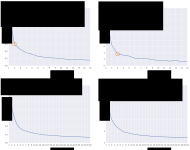
\includegraphics[width=\linewidth]{elbows.pdf}
    \begin{subfigure}{0pt}
        \phantomcaption
        \label{fig:elbows:sub:bv_phylo}
    \end{subfigure}
    \begin{subfigure}{0pt}
        \phantomcaption
        \label{fig:elbows:sub:bv_imb}
    \end{subfigure}
    \begin{subfigure}{0pt}
        \phantomcaption
        \label{fig:elbows:sub:hmp_phylo}
    \end{subfigure}
    \begin{subfigure}{0pt}
        \phantomcaption
        \label{fig:elbows:sub:hmp_imb}
    \end{subfigure}
    \caption[Variances of $k$-means clusters in our test datasets]{
        \textbf{Variances of $k$-means clusters in our test datasets.}
        The figures show the cluster variance for different values of $k$.
        The first row are clusterings of the BV dataset, the second row of the HMP dataset.
        They were clustered using Phylogenetic $k$-means (first column),
        and Imbalance $k$-means (second column), respectively.
        Accordingly, \subref{fig:elbows:sub:bv_phylo} and \subref{fig:elbows:sub:hmp_phylo} use the KR distance,
        while \subref{fig:elbows:sub:bv_imb} and \subref{fig:elbows:sub:hmp_imb} use the euclidean distance
        to measure the variance.
        Orange circles mark potential elbow points.
    }
    \label{fig:elbows}
\end{figure}

The plots for the \ac{BV} dataset in \figref{fig:elbows:sub:bv_phylo} and \subref{fig:elbows:sub:bv_imb}
exhibit the elbow at $k:=2$ and $3$, respectively, which are marked with orange circles.
% exhibit clear elbow points candidates for $k$
These values are consistent with previous findings, c.\,f. \figref{fig:cluster_kmeans_trees} and \figref{fig:kmeans_all}.
On the one hand, Phylogenetic $k$-means splits the samples into a distinct red cluster,
separated from the green and blue clusters,
effectively forming two clusters, which represent the health status of the patients.
On the other hand, Imbalance $k$-means yields three separate clusters in purple, orange, and gray,
which correspond to two clusters for the dominant \taxonname{Lactobacillus} clades,
as well as a cluster for the patients affected by \ac{BV}.

In the plots for the \ac{HMP} dataset, the elbow is less pronounced.
We suspect that this is due to two reasons, as explained in \secref{ch:Clustering:sec:Results:sub:HMPDataset}:
(i) the broad reference tree might not being able to adequately resolve fine-grained differences between samples,
and (ii) nearby body sites might simply be too homogeneous in their metagenomic composition for a clear separation into clusters.
Likely candidates for $k$ are \num{4}--\num{6} for Phylogenetic $k$-means in \figref{fig:elbows:sub:hmp_phylo}
and around \num{7} for Imbalance $k$-means in \figref{fig:elbows:sub:hmp_imb}.
These values are consistent with the number of coherent ``blocks'' of clusters,
as shown in \figref{fig:hmp_kmeans_all_18}.
Clearer results for this dataset might be obtained with other methods for finding ``good'' values for $k$,
although we did not test them here.

% ======================================================================================================================
%     Performance
% ======================================================================================================================

\subsection{Performance}
\label{ch:Clustering:sec:Results:sub:Performance}

The complexity of Phylogenetic $k$-means is in $\mathcal{O}(k \cdot i \cdot n \cdot e)$,
with $k$ clusters, $i$ iterations, and $n$ samples, and $e$ being the number of tree edges,
which corresponds to the number of dimensions in standard euclidean $k$-means.
As the centroids are randomly initialized, the number of iterations can vary;
in our tests, it was mostly below \num{100}.
For the \ac{BV} dataset with \num{220} samples and a reference tree with \num{1 590} edges, using $k:=3$,
our implementation ran \num{9} iterations, needing \SI{35}{\second} and \SI{730}{\mega\byte} of main memory on a single core.
For the \ac{HMP} dataset with \num{9 192} samples and \num{3 824} edges, we used $k:=18$,
which took \num{46} iterations and ran in \SI{2.7}{\hour} on \num{16} cores, using \SI{48}{\giga\byte} memory.

In contrast to this, Imbalance $k$-means neither needs to conduct any expensive tree traversals,
nor take single placement locations into account,
but instead operates on compact vectors, using euclidean distances.
It is hence several orders of magnitude faster than Phylogenetic $k$-means.
For example, using again $k:=18$ for the \ac{HMP} dataset,
the algorithm executed \num{75} iterations in \SI{2}{\second}.
It is thus also applicable to extremely large datasets.

Furthermore, %as the KR distance is used in Phylogenetic $k$-means, %as well as other methods such as Squash Clustering,
our implementation of the KR distance calculation is highly optimized and
outperforms the existing implementation in \toolname{guppy} \cite{Matsen2010} by orders of magnitude.
The KR distance between two samples has a linear computational complexity in both the number of \acp{QS} and the tree size.
As a test case, we computed the pairwise distance matrix between sets of samples.
Calculating this matrix is quadratic in the number of samples,
and is thus expensive for large datasets.
For example, in order to calculate the matrix for the \ac{BV} dataset with \num{220} samples,
\toolname{guppy} can only use a single core and required \SI{86}{\minute}.
Our KR distance implementation \todo{ref to implementation/genesis?} is faster and also supports multiple cores.
It only needed \SI{90}{\second} on a single core; almost half of this time is used for reading input files.
When using \num{32} cores, the matrix calculation itself only took \SI{8}{\second}.
This allows to process larger datasets:
The distance matrix of the \ac{HMP} dataset with \num{9 192} samples placed on a tree with \num{3 824} branches
for instance took less than \SI{10}{\hour} to calculate using \num{16} cores \todo{ref to implementation/genesis?}.
In contrast, \toolname{guppy} needed \num{43} days for this dataset.
As the KR distance is used in Squash Clustering, our re-implementation of this method
is also orders of magnitude faster than the original \toolname{guppy} implementation.

Lastly, in order to achieve additional speedup for even bigger datasets, the mass binning method can be used,
as explained in \secref{ch:Foundations:sec:PhylogeneticPlacement:sub:PlacementProcessing:par:EdgeMasses}.
The performance and the effects of binning on the distance values are shown in \tabref{tab:hmp_binning_error}.

\begin{table}[htb]
\caption[Effect of Branch Binning on the KR Distance of the HMP Dataset]{
    \textbf{Effect of Branch Binning on the KR Distance of the HMP Dataset.}
    Here we show the effect of per-branch placement binning
    on the run-time and on the resulting relative error when calculating the pairwise KR distance matrix between samples,
    by example of the Human Microbiome Project (HMP) \cite{Huttenhower2012,Methe2012} dataset
    (see \appref{supp:sec:DetailsEmpiricalDatasets:sub:HMP} for details).
    Because of the size of the dataset (\num{9192} samples) and reference tree (\num{1914} taxa),
    we executed this evaluation in parallel on \num{16} cores.
    The first row shows the baseline performance, that is, without binning.
}
\label{tab:hmp_binning_error}
{
    \begin{center}
    \begin{tabular}{rrrr}
        \toprule
        Bins    &  Time\,(h:mm) &  Speedup  &  Relative\,$\Delta$ \\
        \midrule
        -     & 9:46   & 1.00   & 0.000000 \\
        256   & 6:58   & 1.40   & 0.000008 \\
        128   & 6:39   & 1.47   & 0.000015 \\
        64    & 6:30   & 1.50   & 0.000035 \\
        32    & 6:25   & 1.52   & 0.000124 \\
        16    & 6:13   & 1.57   & 0.000272 \\
        8     & 6:08   & 1.59   & 0.000669 \\
        4     & 6:07   & 1.60   & 0.002747 \\
        2     & 6:04   & 1.61   & 0.004284 \\
        1     & 5:35   & 1.75   & 0.011585 \\
        \bottomrule
    \end{tabular}
    \end{center}
}
\end{table}

The first row represents the baseline case of using no binning,
where each placement location of the \num{118} million sequences
is taken into account in the computation of the KR distance.
Hence, even binning the masses on each of the \num{3 824} branches of the tree into \num{256} intervals
already yields a substantial speedup.
When using fewer bins per branch, the run-time further decreases,
at the cost of slightly increasing the average relative error.
Still, even when compressing the placement masses into only one bin per branch (that is, just using per-branch masses),
the average relative error of the KR distances is around 1\%, which is acceptable for most applications.
However, considering that the run-time savings are not substantially better for a low number of bins,
we recommend using a relatively large number of bins, e.g., \num{32} or more.
This is because run-times of KR distance calculations also depend on other effects
such as the necessary repeated tree traversals.
We also conducted these tests on the \ac{BV} dataset, were the relative error is even smaller.
However, because of the comparatively small size of this dataset, the run-times are too short for accurate measurements,
and thus not shown here.

% ######################################################################################################################
%         Conclusion and Outlook
% ######################################################################################################################

\section{Conclusion and Outlook}
\label{ch:Clustering:sec:ConclusionOutlook}

In this chapter, we presented two adapted variants of the $k$-means method,
which exploit the structure of phylogenetic placement data to identify clusters of environmental samples.
The methods builds upon ideas such as Squash Clustering and can be applied to substantially larger datasets,
as they construct a pre-defined number of clusters.
They are thus useful to identify similarities between large sets of metagenomic samples.

Phylogenetic $k$-means uses the KR distance to assess sample similarity,
and hence yields cluster assignments that are consistent with Squash Clustering.
Imbalance $k$-means on the other hand is based on edge imbalances,
and thus yields assignments that are consistent with Edge PCA, which also uses edge imbalances.
Furthermore, Imbalance $k$-means operates in the euclidean space instead of mass distributions on trees,
and is therefore several orders of magnitude faster than Phylogenetic $k$-means
and can be applied to very large datasets.

The choice of a reasonable value for $k$ is a general issue in $k$-means clustering.
It might hence be worth to trying more sensitive methods for estimating $k$ than the Elbow method evaluated here.
For future exploration however, other forms of cluster analyses offer more potential.
For example, methods such as soft $k$-means clustering \cite{Dunn1973,Bezdek1981} or density-based methods \cite{Kriegel2011}
could be explored for clustering metagenomic sequence samples.
% by extending them to work on phylogenetic placement data.

The main challenge when adopting such methods to phylogenetic placement data consists in making them phylogeny-aware.
That is, they have to be extended to this type of data by
using mass distributions on trees instead of operating on $\mathbb{R}^d$ vectors in the euclidean space,
%as the underlying space in which the data is modeled.
and using appropriate distances measures such as the KR distance to assess sample similarity.
% The necessary adaptations in the clustering algorithms are not always \todo{what?}
In case of using edge imbalances (instead of edge masses),
the adaptation of existing clustering methods is more straight forward
and might work by plugging in the edge imbalance matrix into existing implementations.

% \todo{cluster centroid diversity ist interessant. plus tax assignment counts a la pierre pro centroid.}

% ######################################################################################################################
%         Conclusion and Outlook
% ######################################################################################################################

\chapter{Conclusion and Outlook}
\label{ch:ConclusionOutlook}

we showed...

in the future...
future work

scrapp: species count estimation, used to discover novelty! (the novelty aspect is mentioned in the foundations chapter!)


% ------------------------------------------
%    Appendices
% ------------------------------------------

\appendix
% ######################################################################################################################
%         Supporting Information
% ######################################################################################################################

\chapter{Supporting Information}
\label{ch:SupportingInformation}

\begin{table}[htb]
\caption[IUPAC notation of nucleobases and ambiguity characters]{
\textbf{IUPAC notation of nucleobases and ambiguity characters.}
The table lists the character representations of nucleobases and their combinations
(which are used to denote ambiguity) as suggested by the IUPAC Commission \cite{IUPAC1970}.
The names and symbols for ambiguity characters are chosen based on bio-chemical properties of the nucleobases.
See \secref{ch:Foundations:sec:SequenceAnalysis:sub:ConsensusSequences} for more information.
}
\label{tab:AmbiguityCharacters}
{
    \newcommand{\mc}[3]{\multicolumn{#1}{#2}{#3}}
    \newcommand{\rb}{\cellcolor{black!12}}
    \begin{center}
    \begin{tabular}{c|l|cccc|c|c}
%     \toprule
%     \hline
    Symbol & Description & \mc{5}{c|}{Represented Bases} & Complement \\
%     \midrule
    \hline
    A & \textbf{A}denine & \rb{} A &  &  &  & 1 & T \\
    C & \textbf{C}ytosine &  & \rb{} C &  &  & 1 & G \\
    G & \textbf{G}uanine &  &  & \rb{} G &  & 1 & C \\
    T & \textbf{T}hymine &  &  &  & \rb{} T & 1 & A \\
    U & \textbf{U}racil &  &  &  & \rb{} U & 1 & A \\
    \hline
    W & \textbf{W}eak & \rb{} A &  &  & \rb{} T & 2 & W \\
    S & \textbf{S}trong &  & \rb{} C & \rb{} G &  & 2 & S \\
    M & a\textbf{M}ino & \rb{} A & \rb{} C &  &  & 2 & K \\
    K & \textbf{K}eto &  &  & \rb{} G & \rb{} T & 2 & M \\
    R & pu\textbf{R}ine & \rb{} A &  & \rb{} G &  & 2 & Y \\
    Y & p\textbf{Y}rimidine &  & \rb{} C &  & \rb{} T & 2 & R \\
    \hline
    B & not A (\textbf{B} comes after A) &  & \rb{} C & \rb{} G & \rb{} T & 3 & V \\
    D & not C (\textbf{D} comes after C) & \rb{} A &  & \rb{} G & \rb{} T & 3 & H \\
    H & not G (\textbf{H} comes after G) & \rb{} A & \rb{} C &  & \rb{} T & 3 & D \\
    V & not T (\textbf{V} comes after T and U) & \rb{} A & \rb{} C & \rb{} G &  & 3 & B \\
    \hline
    N & any \textbf{N}ucleotide (not a gap) & \rb{} A & \rb{} C & \rb{} G & \rb{} T & 4 & N \\
    Z & \textbf{Z}ero &  &  &  &  & 0 & Z
%     \bottomrule
%     \hline
    \end{tabular}
    \end{center}
}
\end{table}

\todo{maybe add the entropy examples from \url{/home/lucas/Dropbox/HITS/manuscripts/automatic-reference-trees/svg} here}

% ######################################################################################################################
%         Empirical Datasets
% ######################################################################################################################

\chapter{Empirical Datasets}
\label{ch:EmpiricalDatasets}

\paperbox{
    This chapter is partially based on the peer-reviewed publications:
}{\paperart \paperpppp}{
    \textbf{Contributions:} Lucas Czech... Alexandros Stamatakis...
}

We used three % four
% Neptrops got kicked out. One result of the neotrop paper was that the sequences are hyper diverse, so no good clusters.
% Furthermore, there is not much meta-data. So not a good dataset for either of the methods...
real world datasets to evaluate our methods:

\begin{itemize}
    \item   \acf{BV} \cite{Srinivasan2012}.
            This small dataset was already analyzed with phylogenetic placement in the original publication.
            We used it as an example of an established study to compare our results to.
            It has \num{220} samples with a total of \num{15 060} unique sequences.
    \item   \acf{NTS} \cite{Mahe2017}.
            \todo{check}
            We already analyzed this medium-sized dataset in its publication and found that
            the sequences are highly diverse and not well covered in existing reference databases.
            This was a particular challenge for classical approaches for metagenomic studies.
            It is thus used as an example of a difficult dataset here.
            It contains \num{154} samples with \num{10 567 804} unique sequences in total.
    \item   \acf{TO} \cite{Karsenti2011,Sunagawa2015,Guidi2016}.
            This world-wide sequencing effort of the open oceans provides a rich set of meta-data,
            such as geographic location, temperature, and salinity.
            Unfortunately, the sample analysis for creating the official data repository is still ongoing.
            % See https://www.embl.de/tara-oceans/start/research/index.html
            We thus were only able to use \num{370} samples with \num{27 697 007} unique sequences.
    \item   \acf{HMP} \cite{Huttenhower2012,Methe2012}.
            This large data repository intends to characterize the human microbiota.
            It contains \num{9192} samples from different body sites with a total of \num{63 221 538} unique sequences.
            There is additional meta-data such as age and medical history, which is available upon special request.
            We only used the publicly available meta-data.
    \item   \todo{mouse gut}
\end{itemize}

Details of the datasets (download links, data statistics, data preprocessing, etc.)
are provided in \todo{S1 Text}. %Supplementary Section \nameref{supp:sec:DetailsEmpiricalDatasets}.
At the time of writing, about one year after we initially downloaded the data,
the \ac{TO} repository has grown to \num{1 170} samples,
while the \ac{HMP} even published a second phase and now comprises \num{23 666} samples of the 16S region.
This further emphasizes the need for scalable methods to analyze such data.

These datasets represent a wide range of environments, number of samples, and sequence lengths.
We use them to evaluate our methods and to exemplify which method is applicable to what kind of data.
To this end, the sequences of the datasets were placed on appropriate phylogenetic \acp{RT} as explained
in \todo{S1 Text}, in order to obtain phylogenetic placements that our methods can be applied to.
In the following, we present the respective results, and also compare our methods to other methods
where applicable.
As the amount and type of available meta-data differs for each dataset,
we could not apply all methods to all datasets.
Lastly, we also report the run-time performance of our methods on these data.

The analyses and figures presented here were conducted on distinct reference alignments and trees.
Firstly, for the \ac{BV} dataset, we used the original set of reference sequences, and re-inferred a tree on them.
Secondly, for the \ac{TO} and \ac{HMP} datasets, we used our Phylogenetic Automatic (Reference) Tree \ac{PhAT} method \cite{Czech2018}
to construct sets of suitable reference sequences from the \toolname{Silva} database \cite{Quast2013,Yilmaz2014}.
We used the 90\% threshold consensus sequences;
see \cite{Czech2018} for details.

For all analyses, we used the following software setup:
Unconstrained maximum likelihood trees were inferred using \toolname{RAxML v8.2.8} \cite{Stamatakis2014}.
% Didn't use any constrained trees in this paper. Thus, don't need the following:
% Constrained trees were inferred with \toolname{Sativa 0.9-55} \cite{Kozlov2016},
% which internally again relies on \toolname{RAxML},
% and offers a convenient way to turn a taxonomy into a constraint tree.
For aligning reads against reference alignments and reference trees,
we used a custom MPI wrapper for \toolname{PaPaRa 2.0} \cite{Berger2011a,Berger2012},
which is available at \cite{PaPaRaMPI}.
We then applied the \texttt{chunkify} procedure as explained in \cite{Czech2018}
to split the sequences into chunks of unique sequences prior to conducting the phylogenetic placement,
in order to minimize processing time.
Phylogenetic placement was conducted using \toolname{EPA-ng} \cite{Barbera2018},
which is a faster and more scalable phylogenetic placement implementation
than \toolname{RAxML-EPA} \cite{Berger2011} and \toolname{pplacer} \cite{Matsen2010}.
Lastly, given the per-chunk placement files produced by \toolname{EPA-ng}, we executed the \texttt{unchunkify} procedure of \cite{Czech2018}
to obtain per-sample placement files. These subsequently served as the input data for the methods presented here.

\begin{table}[htb]
\caption[Overview of the dataset dimensions]{
\textbf{Overview of the dataset dimensions.}
The ``Samples'' columns show how many metagenomic samples there were in the originally downloaded data and
how many of those we actually used for our experiments after filtering out spurious ones.
The columns ``Filtered Sample Sizes'' show how many sequences each of the filtered samples has.
The ``Sequence Count'' columns show the total number of sequences in the filtered samples, and how many of them are unique.
The columns ``Sequence Length'' show statistics of the length of the sequences.
Lastly, the ``Chunks'' column shows into how many chunks of size \num{50 000} the samples were distributed.
}
\label{tab:MetagenomicDatasetsOverview}
{
    \newcommand{\mc}[3]{\multicolumn{#1}{#2}{#3}}
    \begin{center}
    \begin{tabular}{l|rr|rrr|rr|rrr|r}
                        & \mc{2}{c|}{Samples}                      & \mc{3}{c|}{Filtered Sample Sizes}                 & \mc{2}{c|}{Filtered Sequence Count}   & \mc{3}{c|}{Filtered Sequence Length}              & \mc{1}{r}{} \\
    Dataset             & \mc{1}{r}{Source} & \mc{1}{r|}{Filtered} & \mc{1}{r}{Min} & \mc{1}{r}{Max} & \mc{1}{r|}{Avg} & \mc{1}{r}{Total} & \mc{1}{r|}{Unique} & \mc{1}{r}{Min} & \mc{1}{r}{Max} & \mc{1}{r|}{Avg} & Chunks \\
    \hline
    Bacterial Vaginosis &                   &                  220 &                &                &                 &          426,612 &             15,060 &                &                &             226 &      1 \\
    Neotropical Soils   &                   &                  154 &                &                &                 &       50,118,536 &         10,567,804 &                &                &             364 &    212 \\
    Tara Oceans         &                   &                  370 &                &                &                 &       49,023,231 &         27,697,007 &                &                &             128 &    554 \\
    Human Microbiome    &             9,815 &                9,194 &                &                &                 &      118,701,818 &         63,221,538 &                &                &             413 &  1,265 \\
    \end{tabular}
    \end{center}
}
\end{table}

\section{Bacterial Vaginosis}
\label{supp:sec:DetailsEmpiricalDatasets:sub:BV}

We used the Bacterial Vaginosis dataset \cite{Srinivasan2012} in order to compare our novel methods to
existing ones such as Edge PCA and Squash Clustering \cite{Matsen2011a,Evans2012}.
The dataset contains metabarcoding sequences of the vaginal microbiome of \num{220} women,
and was kindly provided by Sujatha Srinivasan.
This small dataset with a total of \num{426 612} query sequences, thereof \num{15 060} unique,
was already analyzed with phylogenetic placement methods in the original publication.
We re-inferred the reference tree of the original publication using the original alignment,
which contains \num{797} reference sequences specifically selected to represent the vaginal microbiome.
As the query sequences were already prepared,
no further preprocessing was applied prior to phylogenetic placement.
The available per-sample quantitative meta-data for this dataset comprises
the Nugent score \cite{Nugent1991}, the value of Amsel's criteria \cite{Amsel1983}, and the vaginal pH value.
We used all three meta-data types in our analyses.

\todo{ from art: }

For testing the accuracy of our unconstrained \taxonname{Bacteria} tree on real data,
we used a vaginal microbiome dataset of 220 women \citep{Srinivasan2012},
which was provided by Sujatha Srinivasan.
See \figref{fig:bv_squash} and \figref{fig:bv_edgepca} for the respective results.
This small dataset with a total of \num{426 612} query sequences, thereof \num{15 060} unique,
was already analyzed with phylogenetic placement methods in the original publication.
We used it as an example of a well-designed study to asses our results using an \ac{PhAT} as reference tree.
In addition to the \taxonname{Bacteria} \ac{PhAT},
we re-inferred the reference tree of the original publication using their alignment,
again using \toolname{RAxML~8.2.8} \citep{Stamatakis2014}.
The query sequences of the dataset were then aligned to our reference tree and alignment,
as well as to the reference alignment of the original publication and our re-inferred tree.
For aligning, we used a custom MPI wrapper of \toolname{PaPaRa~2.0} \citep{Berger2011a,Berger2012},
which is available at \citep{PaPaRaMPI}.
Finally, the query sequences were placed on these trees using \toolname{EPA-ng} \citep{Barbera2018},
and the analyses were subsequently performed as explained in \figref{fig:bv_squash} and \figref{fig:bv_edgepca}.
\todo{the above is not up to date!}

\section{Neotropical Soils}
\label{supp:sec:DetailsEmpiricalDatasets:sub:NTS}

\section{Tara Oceans}
\label{supp:sec:DetailsEmpiricalDatasets:sub:Tara}

The \acf{TO} dataset \cite{Karsenti2011,Sunagawa2015,Guidi2016}
that we used here contains amplicon sequences of protists,
and is available at \url{https://www.ebi.ac.uk/ena/data/view/PRJEB6610}.
% Seawater was filtered from different depths to retain small and large cell sizes (Protists Organisms).
% The DNA was extracted and amplified by PCR.
At the time of download, there were \num{370} samples available
with a total of \num{49 023 231} sequences.
As the available data are raw \texttt{fastq} files,
we followed \cite{FredsMetabarcodingPipeline} to generate cleaned per-sample \texttt{fasta} files.
For this, we used our tool \toolname{PEAR} \cite{Zhang2014} to merge the paired-end reads;
\toolname{cutadapt} \cite{Martin2011} for trimming tags as well as forward and reverse primers;
and \toolname{vsearch} \cite{Rognes2016} for filtering erroneous sequences and
generating per-sample \texttt{fasta} files.
We filtered out sequences below \SI{95}{bps} and above \SI{150}{bps}, to remove potentially erroneous sequences.
No further preprocessing (such as chimera detection) was applied.
This resulted in a total of \num{48 036 019} sequences, thereof \num{27 697 007} unique.
The sequences were then used for phylogenetic placement as explained above.
We placed the sequences on the unconstrained \taxonname{Eukaryota} reference tree obtained via our \ac{PhAT} method \cite{Czech2018},
which comprises \num{2 059} taxa, thereof \num{1 795} eukaryotic sequences.
The remaining \num{264} taxa are \taxonname{Archaea} and \taxonname{Bacteria},
and were included as a broad outgroup.
The \ac{TO} dataset has a rich variety of per-sample meta-data features;
in the context of this paper, we mainly focus on quantitative features such as
temperature, salinity, as well as oxygen, nitrate and chlorophyll content of the water.
Furthermore, each sample has meta-data features indicating the date, longitude and latitude, depth, etc.~of the sampling location.
This data might be interesting for further correlation analyses based on geographical information.
We did not use them here, as for example longitude and latitude would require a more involved method
that also accounts for, e.g., ocean currents.
Furthermore, geographical coordinates yield pairwise distances between samples,
which are not readily usable with our correlation analysis.
Lastly, in order to use features such as the date, that is, in order to analyze samples over time,
the same sampling locations would need to be visited at different times during the year,
which is not the case for the Tara Oceans expedition.

\section{Human Microbiome Project}
\label{supp:sec:DetailsEmpiricalDatasets:sub:HMP}

We used the \acf{HMP} dataset \cite{Huttenhower2012,Methe2012} for testing the scalability of our methods.
In particular, we used the ``HM16STR'' data of the initial phase ``HMP1'',
which are available from \url{http://www.hmpdacc.org/hmp/}.
The dataset consists of trimmed 16S rRNA sequences of the \texttt{V1V3}, \texttt{V3V5}, and \texttt{V6V9} regions.
The data are further divided into a ``by\_sample'' set and a ``healthy'' set,
which we merged in order to obtain one large dataset, with a total of \num{9 811} samples.
We then removed \num{10} samples that were larger than \SI{70}{\mega\byte}
as well as \num{605} samples that had fewer than \num{1 500} sequences,
because we considered them as defective or unreliable outliers.
% because they lack enough detail for properly measuring the KR distance,
Finally, we also removed \num{2} samples that did not have a valid body site label assigned to them.
This resulted in a set of \num{9192} samples
containing a total of \num{118 702 967} sequences with an average length of \SI{413}{bps}.
From these samples, sequences with a length of less than \SI{150}{bps}
as well as sequences longer than \SI{540}{bps} were removed,
as we considered them potentially erroneous.
No further preprocessing (such as chimera detection) was applied.
This resulted in a total of \num{116 520 289} sequences, of which \num{63 221 538} were unique.
We then used the unconstrained \taxonname{Bacteria} tree of our \ac{PhAT} method \cite{Czech2018} for phylogenetic placement.
The tree comprises \num{1 914} taxa, thereof \num{1 797} bacterial sequences.
The remaining \num{117} taxa are \taxonname{Archaea} and \taxonname{Eukaryota},
and were included as a broad outgroup.
Each sample is labeled with one of \num{18} human body site locations where it was sampled.
This is the only publicly available meta-data feature.
% See Table~\ref{tab:hmp_data_overview} for an overview of those labels.

\todo{ from art: }

We used the \acf{HMP} dataset \citep{Huttenhower2012,Methe2012} for further testing our methods
(see Figure~\ref{fig:hmp_mds_epca}).
In particular, we used the ``HM16STR'' data of their initial phase ``HMP1'',
which are available from \url{http://www.hmpdacc.org/hmp/}.
The dataset consists of trimmed 16S rRNA sequences of the \texttt{V1V3}, \texttt{V3V5}, and \texttt{V6V9} regions.
Each sample of the dataset is labeled with the human body site where it was obtained.
See Table~\ref{tab:hmp_data_overview} for an overview of those labels.
The data are further divided into a ``by\_sample'' set and a ``healthy'' set,
which we merged in order to obtain one large dataset, with a total of \num{9 811} samples.
We then removed \num{10} samples that were larger than \SI{70}{\mega\byte}
as well as \num{605} samples that had fewer than \num{1 500} sequences,
because we considered them as outliers,
% because they lack enough detail for properly measuring the KR distance,
and finally \num{2} samples that did not have a valid body site label assigned to them.
This resulted in a set of \num{9192} samples
containing a total of \num{118 702 967} sequences with an average length of \SI{413}{bps}.
From these samples, sequences with a length less than \SI{150}{bps}
as well as sequences longer than \SI{540}{bps} were removed.
No further preprocessing (e.g., chimera detection) was applied.
This resulted in a total of \num{116 520 289} sequences, of which \num{63 221 538} were unique.
These were split into \num{1 265} chunks of size \num{50 000} each, which were subsequently aligned to and
placed on the unconstrained \taxonname{Bacteria} tree with \num{2 059} tips using the steps explained above.
The chunk placements were then transformed again into per-sample placement files,
before finally running the steps explained in Figure~\ref{fig:hmp_mds_epca}.
% see mapseq paper for another example of hmp processing description

% ======================================================================================================================
%     HMP Dataset Labels
% ======================================================================================================================

\begin{table}[htb]
\caption[HMP Dataset Overview]{
\textbf{HMP Dataset Overview.}
The table lists the \num{18} body site labels used by the Human Microbiome Project (HMP) \citep{Huttenhower2012,Methe2012},
and a ``translation'' into the corresponding body region.
We used this dataset to evaluate the applicability of typical analysis methods for phylogenetic placement
using our \acp{PhAT}, see \secref{ch:AutomaticTrees:sec:Evaluation:sub:EmpiricalDatasets:par:HMP} for details.
Furthermore, we evaluated our $k$-means clustering methods on this dataset,
as described in \secref{ch:Clustering:sec:Results:sub:HMPDataset}.
% In order to simplify the visualization in \figref{fig:hmp_mds_epca},
In these evaluations,
we summarized some of the labels into eight location groups, as shown in the third column.
The last column lists how many samples from each body site were used in our evaluation.
}
\label{tab:hmp_data_overview}
{
    \begin{center}
    \begin{tabular}{lllr}
        \toprule
        Body Site                       & Region            & Group             & Samples   \\
        \midrule
        Stool                           & Stool             & Stool             & 600   \\
        Saliva                          & Saliva            & Saliva            & 529   \\
        Tongue Dorsum                   & Mouth (back)      & Mouth (back)      & 610   \\
        Throat                          & Mouth (back)      & Mouth (back)      & 638   \\
        Palatine Tonsils                & Mouth (back)      & Mouth (back)      & 599   \\
        Attached Keratinized Gingiva    & Mouth (front)     & Mouth (front)     & 600   \\
        Hard Palate                     & Mouth (front)     & Mouth (front)     & 566   \\
        Buccal Mucosa                   & Mouth (front)     & Mouth (front)     & 597   \\
        Subgingival Plaque              & Plaque            & Plaque            & 595   \\
        Supragingival Plaque            & Plaque            & Plaque            & 608   \\
        Anterior Nares                  & Nose              & Airways           & 541   \\
        Left Antecubital Fossa          & Arm               & Skin              & 290   \\
        Right Antecubital Fossa         & Arm               & Skin              & 328   \\
        Left Retroauricular Crease      & Ear               & Skin              & 596   \\
        Right Retroauricular Crease     & Ear               & Skin              & 604   \\
        Vaginal Introitus               & Vagina            & Vagina            & 292   \\
        Mid Vagina                      & Vagina            & Vagina            & 298   \\
        Posterior Fornix                & Vagina            & Vagina            & 301   \\
%         N/A                             &                   &                   & 2     \\
        Sum                             &                   &                   & 9192  \\
        \bottomrule
    \end{tabular}
    \end{center}
}
\end{table}

\section{Mouse Gut}
\label{supp:sec:DetailsEmpiricalDatasets:sub:MouseGut}

This dataset was used for the eval of tax assign in \secref{ch:AutomaticTrees:sec:Evaluation:sub:TaxonomicAssignmentProfiling}

CAMI Challenge \citep{Sczyrba2017}.
The CAMI Challenge is a community-driven effort to assess taxonomic profiling methods
using a common set of benchmark data sets.


we utilized the \taxonname{mouse gut} data set of the 2nd CAMI Challenge \citep{Bremges2018}.


More specifically, we used the unpaired HiSeq reads of the mouse gut data set from CAMI,
which comprises \num{64} samples of simulated reads.
The preprocessing involved read de-interleaving following \cite{DeinterleaveFastq},
paired-end read merging using \toolname{PEAR} \citep{Zhang2014},
as well as quality filtering and conversion to \texttt{fasta} using \toolname{VSEARCH2} \citep{Rognes2016}.
This yielded a total of \num{800 341 409} reads.
As our trees are based on small ribosomal subunit sequences,
we also performed read filtering to obtain reads from the 16S rDNA region
(see \secref{ch:Foundations:sec:SequenceAnalysis:sub:Metagenomics}).
This filtering was performed using the protocol of \cite{Logares2014},
which relies on \toolname{HMMER} \citep{Eddy1998,Eddy2009}, and respective profiles for the 16S rDNA locus.
We performed a global identity based de-replication step on the resulting reads that yielded \num{616 405} query sequences.
We aligned these query sequences to our \taxonname{Bacteria} reference alignment
using \toolname{PaPaRa~2.0} \citep{Berger2011a,Berger2012}.
We then performed phylogenetic placement of the aligned query sequences onto the unconstrained and constrained reference trees,
respectively, using \toolname{EPA-ng} \citep{Barbera2018}.
We performed de-de-replication to obtain per-sample data again, %on the \texttt{jplace} file,
resulting in \num{64} \texttt{jplace} files (one per original sample) with placements of the 16S rDNA sequences,
for each of the two trees.


Finally, we performed taxonomic assignment and taxonomic profiling of the per-sample results
using the \texttt{assign} command implemented in \toolname{gappa},
which works analogously to the method used in \toolname{Sativa} \citep{Kozlov2016}.
Its basic steps are described in \appref{ch:PipelineImplementation}.


% ######################################################################################################################
%         Pipeline and Implementation
% ######################################################################################################################

\cleardoublepage

\chapter{Pipeline and Implementation}
\label{ch:PipelineImplementation}

\paperbox{
    This chapter is based on the peer-reviewed publications:
}{\paperart \paperpppp}{
    \textbf{Contributions:} Lucas Czech... Alexandros Stamatakis...
}

\todo{add genesis and gappa logos. because we can.}

The methods described here are implemented in our tool \toolname{gappa},
which is freely available under GPLv3 at \url{http://github.com/lczech/gappa}.
\toolname{gappa} internally uses our C++ library \toolname{genesis},
which offers functionality for working with phylogenies and phylogenetic placement data,
and also contains methods to work with taxonomies, sequences and many other data types.
\toolname{genesis} is also freely available under GPLv3 at \url{http://github.com/lczech/genesis}.

\toolname{gappa} offers a command line interface for conducting typical tasks when working with phylogenetic placements.
The methods that we described here are implemented via the following sub-commands:

\begin{itemize}
    \item \texttt{dispersion}: The command takes a set of jplace files (called samples), and calculates and visualizes
        the Edge Dispersion per edge of the reference tree.
    \item \texttt{correlation}: The command takes a set of jplace samples, as well as a table containing metadata
        features for each sample. It then calculates and visualizes the Edge Correlation with the metadata features per
        edge of the reference tree.
    \item \texttt{phylogenetic-kmeans} and \texttt{imbalance-kmeans}: Performs $k$-means clustering of a set of jplace
        files according to our methods.
    \item \texttt{squash} and \texttt{edgepca}: Reimplementations of the two existing methods \cite{Matsen2011a,Evans2012}.
\end{itemize}

These are the \toolname{gappa} commands that are relevant for this paper.
The tool also offers additional commands that are useful for phylogenetic placement data, such as visualization or filtering.
At the time of writing this manuscript, \toolname{gappa} is under active development,
with more functions planned in the near future.
Lastly, we provide prototype implementations, scripts, data, and other tools
used for the tests and figures in this paper at \url{http://github.com/lczech/placement-methods-paper}.


\todo{ART:}

An implementation of the methods described here is freely available in our tool \toolname{gappa},
which is published under GPLv3 at \url{http://github.com/lczech/gappa}.
\toolname{gappa} is based on our C++ library \toolname{genesis},
which offers functionality concerning phylogenies and phylogenetic placement data,
but also has functions to work with sequences, taxonomies and many other data types.
\toolname{genesis} is also published under GPLv3 and is available at \url{http://github.com/lczech/genesis}.

\toolname{gappa} offers a command line interface for typical tasks of working with phylogenetic placements.
The methods described in this paper are implemented via four sub-commands:

\begin{itemize}
    \item \texttt{phat}: Phylogenetic Automatic (Reference) Tree method.
          The command expects a taxonomy file and a sequence file of a sequence database,
          e.g., \toolname{Silva} \citep{Quast2013,Yilmaz2014},
          as well as the target number of consensus sequences to be generated for the intended phylogeny.
          The result is a \texttt{fasta} file with consensus sequences representing taxonomic clades.
          The command can be further customized, e.g., by changing the consensus sequence method,
          using only a specified subclade of the taxonomy for running the algorithm,
          as well as several detail settings for the method.
          It can also output additional info files that allow to inspect details of the calculations,
          like the number of sequences and their entropy per clade.
    \item \texttt{extract}: Extract/collect placements in specific sub-clades of the tree.
          The command performs the main step of the multilevel placement approach.
          Its input is a set of \texttt{jplace} files containing placements on the backbone tree,
          as well as a file listing the clade name that each taxon of the backbone tree belongs to.
          For each clade, it then writes a new \texttt{jplace} file,
          containing all queries that were placed in that clade with more than a customizable threshold
          of their placement mass.
          \\
          Furthermore, if provided with the sequence files that were used to make the input \texttt{jplace} files,
          the corresponding sequence of each query are also written to \texttt{fasta} files per clade.
          Thus, a per-clade collection of sequences is created, where each result file contains the sequences
          that were placed in this clade of the backbone tree.
          These can then be used for the second level placement on separate clade-specific trees.
    \item \texttt{chunkify}: Split a set of \texttt{fasta} files into chunks of equal size,
          and write abundance maps.
          The command re-names the sequences using a configurable hash function (MD5, SHA1 or SHA256),
          and de-duplicates across all input sequences.
          Its output are chunk files of sequences, as well as an abundance map file for each input sequences file.
          The sequence chunk files can then be used to perform phylogenetic placement
          to obtain per-chunk \texttt{jplace} files.
    \item \texttt{unchunkify}: Take the per-chunk \texttt{jplace} files as well as the abundance map files,
          and generate a \texttt{jplace} for each original sequence file, including the correct abundances.
          This command is the second step of the \texttt{chunkify} command, and reverts its effect,
          so that the resulting \texttt{jplace} files are as if they were created using the original sequence files.
    \item \texttt{assign}: Perform taxonomic assignment using phylogenetic placements.
          While this is not the main focus of this work, we briefly introduce this method here.
          The command uses a taxonomic labeling of the tips of the reference tree
          to annotate all inner branches of the tree with the longest common taxonomic label
          for the induced subtree of the inner branch, in analogy to \toolname{Sativa} \citep{Kozlov2016}.
          Then, each query sequence in the provided \texttt{jplace} files
          is taxonomically assigned according to the labels of the branches where it does have placement mass.
          This can subsequently either be used for taxonomic assignment of the query sequences themselves,
          or to obtain a taxonomic profile of one or more samples.
\end{itemize}

These are the commands of \toolname{gappa} relevant for this paper,
but it also offers more commands that are useful when working with phylogenetic placements.
For details on the commands, and additional potentially useful commands,
see the \toolname{gappa} documentation at \url{https://github.com/lczech/gappa/wiki}.
At the time of writing, it is under active development, and more functions are planned for the near future.
Furthermore, we provide prototype implementations, scripts, data and other tools
used for the tests and figures in this paper at \url{http://github.com/lczech/placement-methods-paper}.

% ######################################################################################################################
%         Publications
% ######################################################################################################################

\cleardoublepage

\chapter{List of Publications}
\label{ch:Publications}

\todo{workshops and conferences, TA}

\begin{enumerate}
    \item \textbf{L. Czech}, S. Berger, D. Krompaß, J. Zhang, P. Kapli, P. Pavlidis, and A. Stamatakis.
        Evolutionary Placement of Short Reads - Methods, Applications, and Visualization.
        Poster at \textit{EMBO/EMBL Symposium: A New Age of Discovery for Aquatic Microeukaryotes}, Heidelberg, Germany, January 2016,
        and at \textit{Hellenic Bioinformatics Conference (HBio) 2016}, Thessaloniki, Greece, November 2016.

    \item F. Mah{\'{e}}, C. de Vargas, D. Bass, \textbf{L. Czech}, A. Stamatakis, E. Lara, D. Singer, J. Mayor, J. Bunge,
        S. Sernaker, T. Siemensmeyer, I. Trautmann, S. Romac, C. Berney, A. Kozlov, E. A. D. Mitchell, C. V. W. Seppey,
        E. Egge, G. Lentendu, R. Wirth, G. Trueba, and M. Dunthorn.
        Parasites dominate hyperdiverse soil protist communities in Neotropical rainforests.
        \textit{Nature Ecology \& Evolution}, 1(4):0091, 2017. \cite{Mahe2017}

    \item \textbf{L. Czech}, J. Huerta-Cepas, and A. Stamatakis.
        A Critical Review on the Use of Support Values in Tree Viewers and Bioinformatics Toolkits.
        \textit{Molecular Biology and Evolution}, 17(4):383--384, 2017. \cite{Czech2017}

    \item T. Flouri, J. Zhang, \textbf{L. Czech}, K. Kobert, and A. Stamatakis.
        An efficient approach to merging paired-end reads and the incorporation of uncertainties.
        In M. Elloumi, editor, \textit{Algorithms for Next-Generation Sequencing Data: Techniques, Approaches and Applications},
        chapter 13, pages 299--326. Springer International Publishing AG, 1 edition, 2017. \cite{Flouri2017}
%         Chapter in \textit{Algorithms for Next-Generation Sequencing Data: Techniques, Approaches and Applications}.
%         1st ed., M. Elloumi, Ed. Springer International Publishing AG, 2017, pp. 299--326. \cite{Flouri2017}

    \item P. Barbera, A. Kozlov, T. Flouri, D. Darriba, \textbf{L. Czech}, and A. Stamatakis.
        Massively Parallel Evolutionary Placement of Genetic Sequences.
        Poster at \textit{ISC 2017 PhD Symposium}, Frankfurt am Main, Germany, June 2017.

    \item C. Berney, A. Ciuprina, S. Bender, J. Brodie, V. Edgcomb, E. Kim, J. Rajan, L. W. Parfrey, S. Adl, S. Audic,
        D. Bass, D. A. Caron, G. Cochrane, \textbf{L. Czech}, M. Dunthorn, S. Geisen, F. O. Glöckner, F. Mah{\'{e}}, C. Quast,
        J. Z. Kaye, A. G. B. Simpson, A. Stamatakis, J. del Campo, P. Yilmaz, and C. de Vargas.
        UniEuk : Time to Speak a Common Language in Protistology!
        \textit{Journal of Eukaryotic Microbiology}, 38(1):42--49, 2017. \cite{Berney2017}

    \item X. Zhou, S. Lutteropp, \textbf{L. Czech}, A. Stamatakis, M. von Looz, and A. Rokas.
        Quartet-based computations of internode certainty provide accurate and robust measures of phylogenetic incongruence.
        \textit{bioRxiv}, 168526, 2017. \cite{Zhou2017}

    \item P. Barbera, A. Kozlov, \textbf{L. Czech}, B. Morel, and A. Stamatakis.
        EPA-ng: Massively Parallel Evolutionary Placement of Genetic Sequences.
        \textit{bioRxiv}, 291658, 2018. \cite{Barbera2018}

    \item D. Bass, \textbf{L.Czech}, B. Williams, C. Berney, M. Dunthorn, F. Mahe, G. Torruella, G. Stentiford, and T. Williams.
        Clarifying the Relationships between Microsporidia and Cryptomycota.
        \textit{Journal of Eukaryotic Microbiology}, 2018.~\cite{Bass2018a}

    \item \textbf{L. Czech}, P. Barbera, and A. Stamatakis.
        Methods for Automatic Reference Trees and Multilevel Phylogenetic Placement.
        \textit{bioRxiv}, 299792, 2018. \cite{Czech2018}

    \item \textbf{L. Czech} and A. Stamatakis.
        Scalable Methods for Post-Processing, Visualizing, and Analyzing Phylogenetic Placements.
        \textit{bioRxiv}, 346353, 2018. \cite{Czech2018a}

    \item \todo{1KITE}
    \item \todo{long reads}
    \item \todo{swarm 3?}
    \item \todo{genesis and gappa}
\end{enumerate}

\clearpage


% ------------------------------------------
%    Literature
% ------------------------------------------

\backmatter

% add toc line
\cleardoublepage
\phantomsection
\addcontentsline{toc}{chapter}{\bibname}

% include also non-cited sources that are in the bib file
% \nocite{*}

% \bibliographystyle{itmabbrv} % mit abgekürzten Vornamen der Autoren
% \bibliographystyle{itmalpha}  % ausgeschriebene Vornamen der Autoren
% \bibliographystyle{IEEEtranSA}	% english style

\bibliographystyle{abbrvnat}
% \bibliographystyle{unsrtnat}
% \bibliographystyle{gerplain} % klappt nicht

% \bibliographystyle{plain}
% % \bibliographystyle{ieee}
% \bibliographystyle{natbib}

\bibliography{thesis}

% ------------------------------------------
%    Indices
% ------------------------------------------

% % the file macros2 defines some special formattings for the index,
% % maybe it should be checked out once the index is needed!
% \cleardoublepage
% \phantomsection
% % \addcontentsline{toc}{chapter}{Index}
% \printindex            % Index, Stichwortverzeichnis

% TODO evtl hier leere seite zum schluss einbauen!
% \clearpage
% \fancyhf{}
% \pagestyle{empty}
% % \newpage
% % \cleardoublepage
% \mbox{}
% % \newpage
% % \mbox{}

\end{document}
